% Template pour faire aide-mémoire
\documentclass[10pt, french]{article}
%% -----------------------------
%% Préambule
%% -----------------------------
% !TEX encoding = UTF-8 Unicode
% LaTeX Preamble for all cheatsheets
% Author : Gabriel Crépeault-Cauchon

% HOW-TO : copy-paste this file in the same directory as your .tex file, and add in your preamble the next command right after you have specified your documentclass : 
% \input{preamble-cheatsht.tex}
% ---------------------------------------------
% ---------------------------------------------

% Extra note : this preamble creates document that are meant to be used inside the multicols environment. See the documentation on internet for further information.

%% -----------------------------
%% Encoding packages
%% -----------------------------
\usepackage[utf8]{inputenc}
\usepackage[T1]{fontenc}
\usepackage{babel}
\usepackage{lmodern}

%% -----------------------------
%% Variable definition
%% -----------------------------
\def\auteur{Gabriel Crépeault-Cauchon / Nicholas Langevin}
\def\BackgroundColor{white}

%% -----------------------------
%% Margin and layout
%% -----------------------------
% Determine the margin for cheatsheet
\usepackage[landscape, hmargin=1cm, vmargin=1.7cm]{geometry}
\usepackage{multicol}

% Remove automatic indentation after section/subsection title.
\setlength{\parindent}{0cm}

% Save space in cheatsheet by removing space between align environment and normal text.
\usepackage{etoolbox}
\newcommand{\zerodisplayskips}{%
  \setlength{\abovedisplayskip}{0pt}%
  \setlength{\belowdisplayskip}{0pt}%
  \setlength{\abovedisplayshortskip}{0pt}%
  \setlength{\belowdisplayshortskip}{0pt}}
\appto{\normalsize}{\zerodisplayskips}
\appto{\small}{\zerodisplayskips}
\appto{\footnotesize}{\zerodisplayskips}

%% -----------------------------
%% URL and links
%% -----------------------------
\usepackage{hyperref}
\hypersetup{colorlinks = true, urlcolor = gray!70!white, linkcolor = black}

%% -----------------------------
%% Document policy (uncomment only one)
%% -----------------------------
%	\usepackage{concrete}
	\usepackage{mathpazo}
%	\usepackage{frcursive} %% permet d'écrire en lettres attachées
%	\usepackage{aeguill}
%	\usepackage{mathptmx}
%	\usepackage{fourier} 

%% -----------------------------
%% Math configuration
%% -----------------------------
\usepackage[fleqn]{amsmath}
\usepackage{amsthm,amssymb,latexsym,amsfonts}
\usepackage{empheq}
\usepackage{numprint}
\usepackage{dsfont} % Pour avoir le symbole du domaine Z

% Mathematics shortcuts

\newcommand{\reels}{\mathbb{R}}
\newcommand{\entiers}{\mathbb{Z}}
\newcommand{\naturels}{\mathbb{N}}
\newcommand{\eval}{\biggr \rvert}
\usepackage{cancel}
\newcommand{\derivee}[1]{\frac{\partial}{\partial #1}}
\newcommand{\prob}[1]{\Pr \left( #1 \right)}
\newcommand{\esp}[1]{\mathrm{E} \left[ #1 \right]} % espérance
\newcommand{\variance}[1]{\mathrm{Var} \left( #1   \right)}
\newcommand{\covar}[1]{\mathrm{Cov} \left( #1   \right)}
\newcommand{\laplace}{\mathcal{L}}
\newcommand{\deriv}[2][]{\frac{\partial^{#1}}{\partial #2^{#1}}}
\newcommand{\e}[1]{\mathrm{e}^{#1}}
\newcommand{\te}[1]{\text{exp}\left\{#1\right\}}
\DeclareMathSymbol{\shortminus}{\mathbin}{AMSa}{"39}



% To indicate equation number on a specific line in align environment
\newcommand\numberthis{\addtocounter{equation}{1}\tag{\theequation}}

%
% Actuarial notation packages
%
\usepackage{actuarialsymbol}
\usepackage{actuarialangle}

%
% Matrix notation for math symbols (\bm{•})
%
\usepackage{bm}
% Matrix notation variable (bold style)
\newcommand{\matr}[1]{\mathbf{#1}}



%% -----------------------------
%% tcolorbox configuration
%% -----------------------------
\usepackage[most]{tcolorbox}
\tcbuselibrary{xparse}
\tcbuselibrary{breakable}

%%
%% Coloured box "definition" for definitions
%%
\DeclareTColorBox{definition}{ o }				% #1 parameter
{
	colframe=blue!60!green,colback=blue!5!white, % color of the box
	breakable, 
	pad at break* = 0mm, 						% to split the box
	title = {#1},
	after title = {\large \hfill \faBook},
}
%%
%% Coloured box "definition2" for definitions
%%
\DeclareTColorBox{definitionNOHFILL}{ o }				% #1 parameter
{
	colframe=blue!60!green,colback=blue!5!white, % color of the box
	pad at break* = 0mm, 						% to split the box
	title = {#1},
	before title = {\faBook \quad },
	breakable
}


%%
%% Coloured box "algo" for algorithms
%%
\newtcolorbox{algo}[ 1 ]
{
	colback = blue!5!white,
	colframe = blue!75!black,
	title=#1,
	fonttitle = \bfseries,
	breakable
}
%%
%% Coloured box "conceptgen" for points adding to a concept's deifintion
%%
\newtcolorbox{conceptgen}[ 1 ]
{
	breakable,
	colback = beaublue,
	colframe = airforceblue,
	title=#1,
	fonttitle = \bfseries
}
%%
%% Coloured box "probch3" pour formules relatives au 3ème chapitre de prob
%%
\newtcolorbox{probch3}[ 1 ]
{
	colback = ruddypink,
	colframe = burgundy,
	fonttitle = \bfseries,	
	breakable,
	title=#1
}
%%
%% Coloured box "formula" for formulas
%%
\newtcolorbox{formula}[ 1 ]
{
	colback = green!5!white,
	colframe = green!70!black,
	breakable,
	fonttitle = \bfseries,
	title=#1
}
%%
%% Coloured box "formula" for formulas
%%
\DeclareTColorBox{algo2}{ o }
{
	enhanced,
	title = #1,
	colback=blue!5!white,	
	colbacktitle=blue!75!black,
	fonttitle = \bfseries,
	breakable,
	boxed title style={size=small,colframe=arsenic} ,
	attach boxed title to top center = {yshift=-3mm,yshifttext=-1mm},
}
%%
%% Coloured box "examplebox" for formulas
%%
\newtcolorbox{examplebox}[ 1 ]
{
	colback = lightmauve,
	colframe = antiquefuchsia,
	breakable,
	fonttitle = \bfseries,title=#1
}
%%
%% Coloured box "rappel" pour rappel de formules
%%
\newtcolorbox{rappel}[ 1 ]
{
	colback = ashgrey,
	colframe = arsenic,
	breakable,
	fonttitle = \bfseries,title=#1
}
%%
%% Coloured box "rappel" pour rappel de formules
%%
\DeclareTColorBox{rappel_enhanced}{ o }
{
	enhanced,
	title = #1,
	colback=ashgrey, % color of the box
%	colframe=blue(pigment),
%	colframe=arsenic,	
	colbacktitle=arsenic,
	fonttitle = \bfseries,
	breakable,
	boxed title style={size=small,colframe=arsenic} ,
	attach boxed title to top center = {yshift=-3mm,yshifttext=-1mm},
}
%%
%% Coloured box "notation" for notation and terminology
%%
\DeclareTColorBox{distributions}{ o }			% #1 parameter
{
	enhanced,
	title = #1,
	colback=gray(x11gray), % color of the box
%	colframe=blue(pigment),
	colframe=arsenic,	
	colbacktitle=aurometalsaurus,
	fonttitle = \bfseries,
	boxed title style={size=small,colframe=arsenic} ,
	attach boxed title to top center = {yshift=-3mm,yshifttext=-1mm},
	breakable
%	left=0pt,
%  	right=0pt,
%    box align=center,
%    ams align*
%  	top=-10pt
}

%% -----------------------------
%% Graphics and pictures
%% -----------------------------
\usepackage{graphicx}
\usepackage{pict2e}
\usepackage{tikz}

%% -----------------------------
%% insert pdf pages into document
%% -----------------------------
\usepackage{pdfpages}

%% -----------------------------
%% Color configuration
%% -----------------------------
\usepackage{color, soulutf8, colortbl}


%
%	Colour definitions
%
\definecolor{blue(munsell)}{rgb}{0.0, 0.5, 0.69}
\definecolor{blue(matcha)}{rgb}{0.596, 0.819, 1.00}
\definecolor{blue(munsell)-light}{rgb}{0.5, 0.8, 0.9}
\definecolor{bleudefrance}{rgb}{0.19, 0.55, 0.91}
\definecolor{blizzardblue}{rgb}{0.67, 0.9, 0.93}
\definecolor{bondiblue}{rgb}{0.0, 0.58, 0.71}
\definecolor{blue(pigment)}{rgb}{0.2, 0.2, 0.6}
\definecolor{bluebell}{rgb}{0.64, 0.64, 0.82}
\definecolor{airforceblue}{rgb}{0.36, 0.54, 0.66}
\definecolor{beaublue}{rgb}{0.74, 0.83, 0.9}
\definecolor{cobalt}{rgb}{0.0, 0.28, 0.67}	% nice light blue-ish
\definecolor{blue_rectangle}{RGB}{83, 84, 244}		% ACT-2004
\definecolor{indigo(web)}{rgb}{0.29, 0.0, 0.51}	% purple-ish
\definecolor{antiquefuchsia}{rgb}{0.57, 0.36, 0.51}	%	pastel dark purple ish
\definecolor{darkpastelpurple}{rgb}{0.59, 0.44, 0.84}
\definecolor{gray(x11gray)}{rgb}{0.75, 0.75, 0.75}
\definecolor{aurometalsaurus}{rgb}{0.43, 0.5, 0.5}
\definecolor{ruddypink}{rgb}{0.88, 0.56, 0.59}
\definecolor{pastelred}{rgb}{1.0, 0.41, 0.38}		
\definecolor{lightmauve}{rgb}{0.86, 0.82, 1.0}
\definecolor{azure(colorwheel)}{rgb}{0.0, 0.5, 1.0}
\definecolor{darkgreen}{rgb}{0.0, 0.2, 0.13}			
\definecolor{burntorange}{rgb}{0.8, 0.33, 0.0}		
\definecolor{burntsienna}{rgb}{0.91, 0.45, 0.32}		
\definecolor{ao(english)}{rgb}{0.0, 0.5, 0.0}		% ACT-2003
\definecolor{amber(sae/ece)}{rgb}{1.0, 0.49, 0.0} 	% ACT-2004
\definecolor{green_rectangle}{RGB}{131, 176, 84}		% ACT-2004
\definecolor{red_rectangle}{RGB}{241,112,113}		% ACT-2004
\definecolor{amethyst}{rgb}{0.6, 0.4, 0.8}
\definecolor{amethyst-light}{rgb}{0.6, 0.4, 0.8}
\definecolor{ashgrey}{rgb}{0.7, 0.75, 0.71}			% dark grey-black-ish
\definecolor{arsenic}{rgb}{0.23, 0.27, 0.29}			% light green-beige-ish gray
\definecolor{amaranth}{rgb}{0.9, 0.17, 0.31}
\definecolor{brickred}{rgb}{0.8, 0.25, 0.33}
\definecolor{pastelred}{rgb}{1.0, 0.41, 0.38}

%
% Useful shortcuts for coloured text
%
\newcommand{\orange}{\textcolor{orange}}
\newcommand{\red}{\textcolor{red}}
\newcommand{\cyan}{\textcolor{cyan}}
\newcommand{\blue}{\textcolor{blue}}
\newcommand{\green}{\textcolor{green}}
\newcommand{\purple}{\textcolor{magenta}}
\newcommand{\yellow}{\textcolor{yellow}}

%% -----------------------------
%% Enumerate environment configuration
%% -----------------------------
%
% Custum enumerate & itemize Package
%
\usepackage{enumitem}
%
% French Setup for itemize function
%
\frenchbsetup{StandardItemLabels=true}
%
% Change default label for itemize
%
\renewcommand{\labelitemi}{\faAngleRight}


%% -----------------------------
%% Tabular column type configuration
%% -----------------------------
\newcolumntype{C}{>{$}c<{$}} % math-mode version of "l" column type
\newcolumntype{L}{>{$}l<{$}} % math-mode version of "l" column type
\newcolumntype{R}{>{$}r<{$}} % math-mode version of "l" column type
\newcolumntype{f}{>{\columncolor{green!20!white}}p{1cm}}
\newcolumntype{g}{>{\columncolor{green!40!white}}m{1.2cm}}
\newcolumntype{a}{>{\columncolor{red!20!white}$}p{2cm}<{$}}	% ACT-2005
% configuration to force a line break within a single cell
\usepackage{makecell}


%% -----------------------------
%% Fontawesome for special symbols
%% -----------------------------
\usepackage{fontawesome}

%% -----------------------------
%% Section Font customization
%% -----------------------------
\usepackage{sectsty}
\sectionfont{\color{\SectionColor}}
\subsectionfont{\color{\SubSectionColor}}

%% -----------------------------
%% Footer/Header Customization
%% -----------------------------
\usepackage{lastpage}
\usepackage{fancyhdr}
\pagestyle{fancy}

%
% Header
%
\fancyhead{} 	% Reset
\fancyhead[L]{Aide-mémoire pour~ \cours ~(\textbf{\sigle})}
\fancyhead[R]{\auteur}

%
% Footer
%
\fancyfoot{}		% Reset
\fancyfoot[R]{\thepage ~de~ \pageref{LastPage}}
\fancyfoot[L]{\href{https://github.com/ressources-act/Guide_de_survie_en_actuariat}{\faGithub \ ressources-act/Guide de survie en actuariat}}
%
% Page background color
%
\pagecolor{\BackgroundColor}




%% END OF PREAMBLE
% ---------------------------------------------
% ---------------------------------------------
%% -----------------------------
%% Variable definition
%% -----------------------------
\def\cours{analyse statistique des risques actuariels}
\def\sigle{ACT-2000}
%
% 	Save more space than default
%
\setlength{\abovedisplayskip}{-15pt}
\setlist{leftmargin=*}
%
%	Extra math symbols
%
\usepackage{mathrsfs}
%
% 	thin space, limits underneath in displays

%% -----------------------------
%% 	Colour setup for sections
%% -----------------------------
\def\SectionColor{cobalt}
\def\SubSectionColor{azure(colorwheel)}
\def\SubSubSectionColor{azure(colorwheel)}
%%%	depth
\setcounter{secnumdepth}{0}
%% -----------------------------

%% -----------------------------
%% Color definitions
%% -----------------------------
\definecolor{indigo(web)}{rgb}{0.29, 0.0, 0.51}
\definecolor{cobalt}{rgb}{0.0, 0.28, 0.67}
\definecolor{azure(colorwheel)}{rgb}{0.0, 0.5, 1.0}
%% -----------------------------
%% Variable definition
%% -----------------------------
%%
%% Matrix notation variable (bold style)
%%
\newcommand\cololine[2]{\colorlet{temp}{.}\color{#1}\bar{\color{temp}#2}\color{temp}}
\newcommand\colbar[2]{\colorlet{temp}{.}\color{#1}\bar{\color{temp}#2}\color{temp}}

\begin{document}

\begin{center}
	\textsc{\Large Contributeurs}\\[0.5cm] 
	\hl{Pendant mon étude de MAS-I, je vais travailler sur cette feuille dans le dépôt de ressources-examens (https://github.com/ressources-act/Ressources-examens).}\\
	\hl{Je vais la remettre ici au mois de septembre.}
\end{center}
\begin{contrib}{MAS-I: Modern Actuarial Statistics I (ACT-2000, ACT-2003, ACT-2005)}
\begin{description}
	\item[aut., cre.] Alec James van Rassel
\end{description}

\textbf{\underline{Référence (manuels, YouTube, notes de cours)}}
En ordre alphabétique :
\begin{description}
	\item[src.]	Coaching Actuaries, Coaching Actuaries MAS-I Manual.
	\item[src.]	Cossette, H., ACT-1002 : Analyse probabiliste des risques actuariels, Université Laval, Québec (QC).
	\item[src.]	Côté, M.-P., ACT-2000 : Analyse statistique des risques actuariels, Université Laval, Québec (QC).
	\item[src.]	Hogg, R.V.; McKean, J.W.; and Craig, A.T., Introduction to Mathematical Statistics, 7th Edition, Prentice Hall, 2013.
	\item[src.]	Luong, A., ACT-2000 : Analyse statistique des risques actuariels, Université Laval, Québec (QC).
	\item[src.]	Luong, A., ACT-2005 : Mathématiques actuarielles IARD I, Université Laval, Québec (QC).
	\item[src.]	Marceau, É., ACT-2001 : Introduction à l'actuariat II, Université Laval, Québec (QC).
	\item[src.]	Starmer, J. (2015). StatQuest. Retrieved from https://statquest.org/.
	\item[src.]	Tse, Y., Nonlife Actuarial Models, Theory Methods and Evaluation, Cambridge University Press, 2009.
	\item[src.]	Weishaus, A., CAS Exam MAS-I, Study Manual, 1st Edition, Actuarial Study Materials, 2018.
\end{description}

\textbf{\underline{Contributeurs}}
\begin{description}
	\item[pfr.]	Sharon van Rassel
	\item[pfr.]	Louis-Philippe Vignault
	\item[pfr.]	Philippe Morin
\end{description}
\end{contrib}

\begin{distributions}[Cours reliés]
\begin{description}
	\item[ACT-2000]	Analyse statistique des risques actuariels
	\item[ACT-2003]	Modèles linéaires en actuariat
	\item[ACT-2005]	Mathématiques actuarielles IARD I
	\item[ACT-2009]	Processus stochastiques
\end{description}

En partie : mathématiques actuarielles vie I (\textbf{ACT-2004}), séries chronologiques (\textbf{ACT-2010}), introduction à l'actuariat II (\textbf{ACT-2001}) et méthodes numériques (\textbf{ACT-2002}).
\end{distributions}


\begin{rappel_enhanced}[Motivation]
Inspiré par la chaîne de vidéos YouTube \href{https://www.youtube.com/user/joshstarmer}{\color{azure(colorwheel)}StatQuest} et mon étude pour MAS-I, je crée cette feuille dans le but de simplifier tous les obstacles que j'ai encourus dans mon apprentissage des statistiques et ainsi simplifier la vie des étudiants en actuariat.

L'objectif est d'expliquer les concepts statistiques de façon claire et concise. Je vous prie de me faire part de tous commentaires et de me signaler toute erreur que vous trouvez! 
\end{rappel_enhanced}

\newpage

\raggedcolumns
\begin{multicols*}{2}

\part{Analyse statistique des risques actuariels}

\section{Échantillonnage et statistiques}
\begin{distributions}[Notation]
\begin{description}
	\item[$X$]	Variable aléatoire d'intérêt $X$ avec fonction de densité $f(x; \theta)$;
	\item[$\Theta$]	Ensemble des valeurs possible pour le paramètre $\theta$ tel que \lfbox[formula]{$\theta \in \Theta$};
		\begin{itemize}
		\item	Par exemple, pour une loi normale $\Theta	=	\{(\mu, \sigma^{2}): \sigma^{2} > 0, -\infty < \mu < \infty\}$.
		\end{itemize}
	\item[$\{X_{1}, \dots, X_{n}\}$]	Échantillon de taille $n$.
		\begin{itemize}
		\item	On pose que les observations ont la même distribution que $X$;
		\item	On pose habituellement l'indépendance entre les observations;
		\item	L'indépendance et la distribution identique rend l'échantillon un \textbf{échantillon aléatoire};
		\item	Lorsque nous avons des observations, ont dénote l'échantillon par $\{x_{1}, \dots, x_{n}\}$ pour représenter des \textit{réalisations} de l'échantillon.
		\end{itemize}
\end{description}
\end{distributions}


%%%%%%%%	%%%%	%%%%	%%%%	%%%%	%%%%	%%%%	%%%%	%%%%	
%%%%		À rajouter éventuellement	%%%%	
%%%%%%%%	%%%%	%%%%	%%%%	%%%%	%%%%	%%%%	%%%%	%%%%	

%\subsection{Distributions d'échantillonnage}
%%	Contenu à y inclure
%	Postulat de normalité
%		Moyenne échantillonnale
%		Variance échantillonnale
%		Statistique T
%		Statistique F
%	Échantillons de distribution inconnue
%		Théorème centrale limite

\columnbreak
\section{Vraisemblance}
\begin{distributions}[Notation]
\begin{description}
	\item[$\mathcal{L}(\theta; \bm{x})$]	Fonction de vraisemblance de $\theta$ en fonction des observations $\bm{x}$;
	\item[$\{X_{1}, \dots, X_{n}\}$]	Échantillon de $n$ observations.
		\begin{itemize}[leftmargin = *]
		\item	Si les $n$ observations sont indépendantes entres-elles et proviennent de la même distribution paramétrique (identiquement distribué) c'est un \textbf{échantillon aléatoire} \textbf{(iid)};
		\item	On peut le dénoter comme $\{X_{n}\}$.
		\end{itemize}
\end{description}
\end{distributions}

On peut voir la fonction de densité $f(x; \theta)$ comme étant une fonction du paramètre inconnu $\theta$ avec $x$ fixé; ceci est la fonction de vraisemblance $\mathcal{L}(\theta; \bm{x})$.
Pour bien saisir ce que représente la fonction de vraisemblance $\mathcal{L}(\theta; \bm{x})$, il faut songer à ce que représente $f(x; \theta)$. \\
$f(x; \theta)$ est une fonction qui fait varier $x$ pour un (ou plusieurs) paramètre $\theta$ fixe. Alors, $\mathcal{L}(\theta; \bm{x})$ est une fonction qui fait varier $\theta$ pour un "paramètre" $\bm{x}$ fixé; ce que l'on considère habituellement comme étant "$x$" est en fait $\theta$ pour la fonction de vraisemblance!

\columnbreak
\section{Qualité de l'estimateur}

La première section traite de \guillemotleft \textbf{estimateurs ponctuels} \guillemotright. 
C'est-à-dire, on produit une seule valeur comme notre meilleur essai pour déterminer la valeur de la population inconnue.
Intrinsèquement, on ne s'attend pas à ce que cette valeur (même si c'en est une bonne) soit la vraie valeur exacte.\\

Une hypothèse plus utile à des fins d'interprétation est plutôt un \textbf{\hyperref[sec:int-estimation]{estimateur par intervalle}}; au lieu d'une seule valeur, il retourne un intervalle de valeurs plausibles qui peuvent toutes être la vraie valeur. 
Le type principal d'\textit{estimateur par intervalle} est \textit{l'intervalle de confiance} traité dans la deuxième sous-section.\\

En bref:
\begin{description}
	\item[Estimateur ponctuel]	L'estimateur $\hat{\theta}_{n}$ assigne une valeur précise à $\theta$ selon l'échantillon.
	\item[Estimateur par intervalle]	Un \textit{intervalle aléatoire}, construit avec l'échantillon aléatoire, ayant une certaine probabilité de contenir la vraie valeur $\theta$.
\end{description}


\subsection{Estimation ponctuelle}

\subsubsection{Biais}
\begin{distributions}[Notation]
\begin{description}[font = \normalfont]
	\item[$\theta$]	Paramètre inconnu à estimer;
		\begin{itemize}
		\item	Dans le cas multivarié, on a un vecteur $\bm{\theta}$ et on défini un ensemble des valeurs possibles $\bm{\Theta}$;
		\item	Par exemple, pour une loi Gamma $\bm{\theta}	=	\{\alpha, \beta\}$ et puisque ces paramètres sont strictement positif $\bm{\Theta}	=	\{\mathbb{R}^{+}, \mathbb{R}^{+}\}$.
		\end{itemize}
	\item[$\hat{\theta}_{n}$]	Estimateur de $\theta$ basé sur $n$ observations;
		\begin{itemize}[leftmargin = *]
		\item	Souvent, on simplifie et écrit $\hat{\theta}$.
		\end{itemize}
	\item[$\text{B}(\hat{\theta}_{n})$]	Biais d'un estimateur $\theta_{n}$.
\end{description}
\end{distributions}

Lorsque nous avons un estimateur $\hat{\theta}_{n}$ pour un paramètre inconnu $\theta$ on espère que, \textbf{en moyenne}, ses erreurs de prévision seront nulles. 
On peut alors trouver $\text{E}[\hat{\theta}_{n} | \theta]$; soit, l'espérance de l'estimateur lorsque $\theta$ est la vraie valeur du paramètre.	\\
Par la suite, on calcule son \textbf{biais} $\text{B}(\hat{\theta}_{n})$ dans la prévision de cette vraie valeur du paramètre:
\begin{algo}{Biais d'un estimateur}
\begin{align*}
	\text{B}(\hat{\theta}_{n}) 
	&= 	\text{E}[\hat{\theta}_{n} | \theta] - \theta
\end{align*}
\tcbline
\begin{description}
	\item[Estimateur sans biais]	lorsque le biais d'un estimateur est nul:
		 \[
		 	\text{B}(\hat{\theta}_{n}) = 0
		 \]
	\item[Estimateur asymptotiquement sans biais]	lorsque le biais d'un estimateur tends vers 0 alors que le nombre d'observations sur lequel il est basé tends vers l'infini: 
		\[
			\limz{n}{\infty}\text{B}(\hat{\theta}_{n}) = 0
		\]
\end{description}
\end{algo}

Cependant, le biais n'indique pas la variabilité des prévisions de l'estimateur $\hat{\theta}_{n}$. Une bonne analogie pour comprendre ce qui nous manque est d’imaginer une personne ayant ses pieds dans de l'eau bouillante et sa tête dans un congélateur; \textbf{en moyenne}, il est correct, mais \textbf{en réalité} il est très inconfortable. Des estimateurs non biaisés seront toujours proches de la vraie valeur, mais ce n'est pas suffisant qu'ils soient bons \textit{en moyenne}. On évalue donc la variabilité d'un estimateur avec sa variance $\text{Var}(\hat{\theta}_{n})$.

%\columnbreak
\subsubsection{Borne Cramér-Rao}
\label{sec:cramer_rao}

\begin{distributions}[Notation]
\begin{description}
	\item[$S(\theta)$]	Fonction de Score, \lfbox[formula]{$S(\theta)	=	\deriv{\theta}{\ln f(\theta; x)}$};
	\item[$\bm{I}_{n}(\theta)$]	Matrice d'information de Fisher d'un échantillon aléatoire $\bm{X}$;
		\begin{itemize}
		\item	La matrice d'information Fisher pour un seule observation sera donc dénotée $\bm{I}(\theta)$ ;
		\item	On obtient une "matrice" lorsque nous estimons plusieurs paramètres et donc $\theta$ n'est pas un scalaire.
		\end{itemize}
	\item[$\hat{\theta}^{EMV}$]	Estimateur du maximum de vraisemblance de $\theta$.
\end{description}
\end{distributions}

Lorsque l'on analyse la variance d'un estimateur \underline{sans biais}, on débute par définir la \hyperlink{cramer-rao}{\textbf{borne inférieure de Cramér-Rao}} de sa variance $\text{Var}(\hat{\theta}_{n})$. Cette borne utilise \textbf{la matrice d'information de Fisher} $\bm{I}_{n}(\theta)$:

\begin{algo}{\hypertarget{cramer-rao}{Borne inférieure Cramér-Rao}}
Sous \hyperlink{reg_cond}{\color{blue!40!green!80!black}certaines conditions de régularité},
\begin{align*}
	\text{Var}(\hat{\theta}_{n}) 
	&\geq	\frac{1}{\bm{I}_{n}(\theta)}
\end{align*}
où
\begin{align*}
	\bm{I}(\theta) 
	&=	\text{E}\left[\Big(\deriv{\theta}{} \ln f(\theta; x)\Big)^{2}\right]	
	\overset{\text{iid}}{\equiv}	\text{E}\left[{\color{red}\shortminus}\deriv[2]{\theta}{\ln f(\theta; x)}	\right]	\\
	\bm{I}_{n}(\theta) 
	&=	\text{E}\left[\Big(\deriv{\theta}{} \ln \mathcal{L}(\theta; \bm{x})\Big)^{2}\right]	
	\overset{\text{iid}}{\equiv}	\text{E}\left[{\color{red}\shortminus}\deriv[2]{\theta}{\ln \mathcal{L}(\theta; \bm{x})}\right]	
\end{align*}
\paragraph{Note}	Dans le cas d'un échantillon aléatoire (alias, les données sont iid) on obtient la deuxième équation et \lfbox[formula]{$\bm{I}_{n}(\theta)	=	n\bm{I}(\theta)$.}
\end{algo}

\subsubsection*{Détails sur la borne Cramér-Rao}
Cette borne est rarement comprise et sur la base de \hyperlink{https://www.youtube.com/watch?v=igQIsYAlKlY}{\color{blue}ce vidéo} et \hyperlink{https://www.youtube.com/watch?v=i0JiSddCXMM}{\color{blue}ce vidéo} je me lance dans l'explication de son intuition. Si vous ne comprenez pas à partir de mes explications, je vous suggère fortement d'allez regarder les vidéos puisque c'est un concept qui va réapparaître plus tard dans le bac.\\

Premièrement, on définit l'utilité des deux premières dérivées:
\begin{description}
	\item[$\frac{\partial}{\partial\theta} \mathcal{L}(\theta)$]: Représente le \og \textit{rate of change}\fg{} de la fonction;
	\item[$\frac{\partial^{2}}{\partial\theta^{2}} \mathcal{L}(\theta)$]: Représente la concavité de la fonction; on peut y penser comme sa forme.
\end{description}

L'estimateur $\hat\theta^{\texttt{EMV}}$ du paramètre $\theta$ d'une distribution est obtenu en posant la première dérivée de sa fonction de vraisemblance $\mathcal{L}(\theta ; x)$ égale à 0. Alors, la première dérivée de $\mathcal{L}(\theta; \bm{x})$ est nulle au point $\theta = \hat\theta^{\texttt{EMV}}$. \\

Puisque ce point maximise la fonction, la dérivée va augmenter avant et diminuer après.
%Puisque ce point maximise la fonction, la dérivée sera négative par la suite! \\
%On ajoute alors un négatif à la définition de la matrice d'information fisher (la deuxième forme) pour plus facilement comparer la décroissance (négative) et la croissance (positive) de la dérivée. \\
Cependant, plusieurs fonctions peuvent avoir le même \textbf{point} où elles sont maximisées tout en étant complètement différentes:

\tikzset{every picture/.style={line width=0.75pt}} %set default line width to 0.75pt        

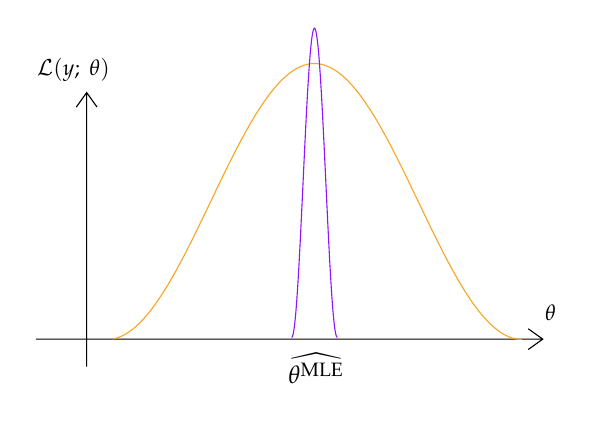
\begin{tikzpicture}[x=0.75pt,y=0.75pt,yscale=-1,xscale=1]
%uncomment if require: \path (0,300); %set diagram left start at 0, and has height of 300

%Shape: Axis 2D [id:dp33309643030277414] 
\draw  (48,169.8) -- (292.17,169.8)(72.42,51) -- (72.42,183) (285.17,164.8) -- (292.17,169.8) -- (285.17,174.8) (67.42,58) -- (72.42,51) -- (77.42,58)  ;
%Shape: Wave [id:dp761793702798415] 
\draw  [color={rgb, 255:red, 245; green, 166; blue, 35 }  ,draw opacity=1 ] (282.17,170) .. controls (264.07,170) and (248.47,137.57) .. (232.17,103.5) .. controls (215.86,69.43) and (200.26,37) .. (182.17,37) .. controls (164.07,37) and (148.47,69.43) .. (132.17,103.5) .. controls (116.77,135.67) and (102,166.38) .. (85.17,169.7) ;
%Shape: Wave [id:dp8411747217824341] 
\draw  [color={rgb, 255:red, 144; green, 19; blue, 254 }  ,draw opacity=1 ] (193.17,169) .. controls (191.18,169) and (189.46,132.67) .. (187.67,94.5) .. controls (185.87,56.33) and (184.16,20) .. (182.17,20) .. controls (180.18,20) and (178.46,56.33) .. (176.67,94.5) .. controls (174.87,132.67) and (173.16,169) .. (171.17,169) ;

% Text Node
\draw (183,184) node  [font=\small] [align=left] {$\displaystyle \widehat{\theta ^{\text{MLE}}}$};
% Text Node
\draw (296,157) node  [font=\footnotesize] [align=left] {$\displaystyle \theta $};
% Text Node
\draw (66,40) node  [font=\footnotesize] [align=left] {$\displaystyle \mathcal{L}( y;\ \theta )$};


\end{tikzpicture}

Clairement, la courbe \textcolor{amethyst}{en mauve} aura plus de points près de $\hat{\theta}^{\text{EMV}}$ que la courbe en \textcolor{orange}{orange}. Afin de comparer les différents estimateurs, on cherche à quantifier l'étendu, ou la variance, de leurs formes. 
La deuxième dérivée sert donc à mesurer la \textit{forme}, ou \textbf{concavité}, de la fonction de vraisemblance et comparer des estimateurs plus adéquatement. \\

Ce faisant, la deuxième dérivée permet d'être plus certain d'avoir le bon estimateur. Il s'ensuit que \lfbox[tight, background-color = palechestnut!60!white, border-color = white]{la variance ne peut pas être moins que l'estimateur du maximum} \lfbox[tight, background-color = palechestnut!60!white, border-color = white]{de vraisemblance évalué au point où la concavité est maximisée}. Alors on peut penser à la forme à ce point comme $\bm{I}(\theta) =$ \og courbe \fg{}. \\

Finalement, on veut comprendre pourquoi $1/\text{\og curve \fg{}}$ et non juste $\text{\og courbe \fg{}}$. On déduit de la fraction que plus la concavité \og courbe \fg{} est élevée, alors plus la variance sera faible. Si la concavité de la fonction est très large, et donc il y a un grand étendue, il y a moins de points près de $\hat\theta^{\text{EMV}}$. Donc:
\begin{equation*}
	\text{Var}(\hat\theta^{\text{EMV}}) 
	\overset{\text{dépend}}{\sim} \frac{1}{\text{\og courbe \fg{}}}	\\
\end{equation*}

On observe alors que la limite lorsque la \og courbe \fg{} tend vers l'infini implique une variance nulle. On dit donc que la distribution de l'estimateur est "asymptotiquement normale" tel que $\hat\theta^{\text{EMV}} \overset{a.s.}{\rightarrow} \mathcal{N}\Big(\mu = \theta, \sigma^{2} = \frac{1}{\bm{I}(\theta)}\Big)$ où a.s. veut dire \hyperlink{asympto}{asymptotiquement}.

\columnbreak
\subsubsection{Efficacité}
\begin{distributions}[Notation]
\begin{description}[font = \normalfont]
	\item[$\text{eff}(\hat{\theta}_{n})$]	Efficacité d'un estimateur $\hat{\theta}_{n}$;
	\item[$\text{eff}(\hat\theta_{n}, \tilde\theta_{n})$]	Efficacité de l'estimateur $\hat{\theta}_{n}$ relatif à l'estimateur $\tilde{\theta}_{n}$.
\end{description}
\end{distributions}

Avec le concept de l'information de Fisher, on défini \textbf{l'efficacité d'un estimateur} comme le ratio de la borne Cramér-Rao sur la variance de l'estimateur:
\begin{algo}{Efficacité d'un estimateur}
\begin{align*}
	\text{eff}(\hat{\theta}_{n})
	&=	\frac{\text{Var}(\hat{\theta}_{n})^{\text{Rao}}}{\text{Var}(\hat{\theta})} 
	=	\frac{1}{\bm{I}(\theta)\text{Var}(\hat{\theta})}
\end{align*}
\tcbline
\begin{description}
	\item[Estimateur \og \textit{efficient} \fg{}]	Lorsque la variance de l'estimateur $\text{Var}(\hat{\theta}_{n})$ est égale à la borne de Cramér-Rao.
		\begin{align*}
		\text{eff}(\hat{\theta}_{n}) = 1
		\end{align*}
	\begin{itemize}[leftmargin = *]
	\item	Étant égale à la borne, il \textit{doit} être l'estimateur avec la plus petite de tous les estimateurs sans biais.\\
	 		On dit qu'il est le \og \textbf{\textit{Minimum Variance Unbiased Estimator (MVUE)}} \fg{}. 
	\end{itemize}
\end{description}
\end{algo}

De plus, on peut généraliser cette formulation pour obtenir l'efficacité relative d'un estimateur à un autre:
\begin{algo}{Efficacité relative}
\begin{align*}
	\text{eff}(\hat\theta_{n}, \tilde\theta_{n})
	&=	\frac{\text{Var}(\hat\theta_{n})}{\text{Var}(\tilde\theta_{n})}		\\
\end{align*}
où les estimateurs $\hat\theta_{n}$ et $\tilde\theta_{n}$ sont sans biais.
\tcbline
Lorsque:
\begin{description}[font = \normalfont]
	\item[$\text{eff}(\hat\theta_{n}, \tilde\theta_{n}) < 1$:]	L'estimateur $\hat{\theta}_{n}$ est plus efficace que l'estimateur $\tilde{\theta}_{n}$, \\
	et vice-versa si $\text{eff}(\hat\theta_{n}, \tilde\theta_{n}) > 1$.
\end{description}
\end{algo}

\columnbreak
\subsubsection{Convergence}
Nous pouvons également évaluer si un estimateur converge avec des très grands échantillons; ceci évalue si un estimateur est cohérent. Un estimateur $\hat{\theta}_{n}$ est dit d'être \og \textit{\textbf{consistent}} \fg{} si la probabilité que sa prévision $\hat{\theta}$ du paramètre $\theta$ diffère de la vraie valeur par une erreur, près de 0, $\epsilon$ tend vers 0 alors que la taille de l'échantillon $n$ tend vers l'infini:
\begin{algo}{Convergence (\textbf{consistency}) d'un estimateur}
\begin{align*}
	\underset{n \rightarrow \infty}{\lim} \Pr(\big| \hat{\theta}_{n} - \theta \big| > \epsilon) = 0, \quad \epsilon > 0
\end{align*}
\end{algo}

Ce critère pour qu'un estimateur $\hat{\theta}_{n}$ soit \og \textit{consistent} \fg{} peut être satisfait lorsque: 
\begin{enumerate}
	\item	l'estimateur est \hypertarget{asympto}{\textbf{asymptotiquement sans biais}};
		\begin{align*}
		\limz{n}{\infty} \text{B}(\hat{\theta}_{n}) = 0
		\end{align*}
	\item	la \textbf{variance de l'estimateur tend vers 0}.
		\begin{align*}
		\limz{n}{\infty} \text{Var}(\hat{\theta}_{n}) = 0
		\end{align*}
\end{enumerate}

D'ailleurs, nous avons déjà raisonné ceci avec \hyperlink{cramer-rao}{la borne inférieure Cramér-Rao}.

Cependant, l'inverse n'est pas vrai---qu'un estimateur soit \og \textit{consistent} \fg{} n'implique pas que sa variance ni que son biais tendent vers 0.\\

Malgré la nature plaisante de la convergence d'un estimateur, beaucoup d'estimateurs ont cette propriété. 
Nous voulons alors une mesure qui n'indique pas seulement qu'un estimateur arrive près de la bonne valeur souvent \textit{(alias, une très petite variance)}, mais qu'il est mieux que d'autres estimateurs.
De plus, dût à la sélection arbitraire de l'erreur $\epsilon$ pour la \textit{consistency} d'un estimateur, il est possible de la choisir malicieusement afin de faire parler les données comme on le souhaite. 

\subsubsection*{Détails sur la convergence}
On reprend les résultats de la section précédente en expliquant plus en détails la mathématique sous-jacente.\\

\begin{definitionNOHFILLsub}[Convergence en probabilité]
\begin{distributions}[Notation]
\begin{description}
	\item[$\{Y_{n}\}$]	Séquence de variables aléatoires;
	\item[$Y$]	Variable aléatoire comprise dans $\{Y_{n}\}$.
\end{description}
\end{distributions}

On dit que $Y_{n}$ converge en probabilité à $Y$ si \lfbox[conditions]{$\forall \varepsilon > 0$}, 
\begin{align*}
	\limz{n}{\infty} \Pr\left[|Y_{n}	-	Y|	\geq	\varepsilon\right]	
	&=	0
\end{align*}
%%%	--------------------
%%%	NOTES:
%%%	+	\geq ou > ???
%%%	--------------------
ou de façon équivalente,
\begin{align*}
	\limz{n}{\infty} \Pr\left[|Y_{n}	-	Y|<	\varepsilon\right]	
	&=	1
\end{align*}

On dénote la convergence en probabilité par: \lfbox[formula]{$Y_{n}	\overset{P}{\rightarrow}	Y$.}
\end{definitionNOHFILLsub}

\paragraph{Note:}	La convergence en probabilité est d'ailleurs le théorème sous-jacent à la loi faible des grands nombres vue en prob.

\begin{rappel}{Loi faible des grands nombres}
\begin{distributions}[Notation]
\begin{description}
	\item[$\{Y_{n}\}$]	Séquence de variables aléatoires iid avec moyenne $\mu$ et variance $\sigma^{2}$ où \lfbox[conditions]{$\sigma^{2}	<	\infty$};
	\item[$\overline{X}_{n}$]	Moyenne empirique.
\end{description}
\end{distributions}

On pose que \lfbox[formula]{$\overline{X}_{n}	\overset{P}{\rightarrow}	\mu$.}
\end{rappel}

\begin{definitionNOHFILLsub}[Théorèmes résultant de la convergence en probabilité]
Soit \lfbox[conditions]{$X_{n}	\overset{P}{\rightarrow}	X$} et \lfbox[conditions]{$Y_{n}	\overset{P}{\rightarrow}	Y$}. Alors \lfbox[formula]{$X_{n} + Y_{n}	\overset{P}{\rightarrow}	X + Y$}.\\
Soit \lfbox[conditions]{$X_{n}	\overset{P}{\rightarrow}	X$} et une \lfbox[conditions]{constante $a$}. Alors \lfbox[formula]{$aX_{n}	\overset{P}{\rightarrow}	aX$}.\\
Soit \lfbox[conditions]{$X_{n}	\overset{P}{\rightarrow}	a$} et la \lfbox[conditions]{fonction $g(\cdot)$ continue à $a$}. Alors \lfbox[formula]{$g(X_{n})	\overset{P}{\rightarrow}	g(a)$}.\\
Soit \lfbox[conditions]{$X_{n}	\overset{P}{\rightarrow}	X$} et la \lfbox[conditions]{fonction continue $g(\cdot)$}. Alors \lfbox[formula]{$g(X_{n})	\overset{P}{\rightarrow}	g(X)$}.\\
Soit \lfbox[conditions]{$X_{n}	\overset{P}{\rightarrow}	X$} et \lfbox[conditions]{$Y_{n}	\overset{P}{\rightarrow}	Y$}. Alors \lfbox[formula]{$X_{n}Y_{n}	\overset{P}{\rightarrow}	XY$}.
\end{definitionNOHFILLsub}

\begin{definitionNOHFILL}[\og \textit{Consistency} \fg{}]
\begin{distributions}[Notation]
\begin{description}
	\item[$Y$]	Variable aléatoire avec une distribution paramétrique de paramètre $\theta$;
	\item[$\{Y_{1}, Y_{2}, \dots, Y_{n}\}$]	Échantillon de la distribution de $Y$;
	\item[$\hat{\theta}_{n}$]	Estimateur de $\theta$.
\end{description}
\end{distributions}

On dit que $\hat{\theta}_{n}$ est un estimateur \og \textit{consistent} \fg{} si \lfbox[formula]{$\hat{\theta}_{n}	\overset{P}{\rightarrow}	\theta$}.
\end{definitionNOHFILL}


\subsubsection{Erreur quadratique moyenne}
\begin{distributions}[Notation]
\begin{description}
	\item[$\text{MSE}_{\hat{\theta}_{n}}(\theta)$]	Erreur quadratique moyenne d'un estimateur $\hat{\theta}_{n}$
\end{description}
\end{distributions}

On défini alors l'\textbf{Erreur Quadratique Moyenne} (EQM), ou \textbf{Mean Squared Error (MSE)}, permettant de comparer les différents estimateurs ayant tous une bonne \textit{consistency} en assurant une cohérence d'interprétation. Cette mesure permet de quantifier l'écart entre un estimateur $\hat{\theta}_{n}$ et le vrai paramètre $\theta$.

\begin{algo}{Erreur Quadratique Moyenne (Mean Squared Error)}
\begin{align*}
	\text{MSE}_{\hat\theta}(\theta)
	&=	\text{E}[(\hat{\theta}_{n} - \theta)^{2}]
	\Leftrightarrow	\text{Var}(\hat{\theta}_{n}) + \left[\text{B}(\hat{\theta}_{n})\right]^{2}
\end{align*}
\end{algo}

En combinant tous ces critères, le meilleur estimateur est alors l'estimateur \textbf{sans biais} ayant la \textbf{plus petite variance} possible parmi tous les estimateurs \textit{sans biais}. C'est-à-dire, le \textbf{Uniformly Minimum Variance Unbiased Estimator \textit{(UMVUE)}}.

\columnbreak

\subsection{Estimation par intervalles}
\label{sec:int-estimation}
\begin{distributions}[Notation]
\begin{description}
	\item[$\hat{\theta}_{L}$ et $\hat{\theta}_{U}$]	Fonctions de l'échantillon aléatoire $\{X_{1}, \dots, X_{n}\}$ où \icbox[red][palechestnut]{$\hat{\theta}_{L} < \hat{\theta}_{U}$};
	\item[$(\hat{\theta}_{L}, \hat{\theta}_{U})$]	Intervalle de confiance de $100(1 - \alpha)\%$ de $\theta$ si \icbox[red][palechestnut]{$\Pr(\hat{\theta}_{L} \leq \theta \leq \hat{\theta}_{U}) = 1 - \alpha$};
		\begin{itemize}
		\item	Avec les réalisations, on a un intervalle de nombres réels $(\hat{\theta}_{l}, \hat{\theta}_{u})$.
		\end{itemize}
	\item[$(1 - \alpha)$]	Niveau de confiance de l'intervalle où \lfbox[conditions]{$\alpha \in (0, 1)$}.
\end{description}
\end{distributions}

Le type principal d'estimateur par intervalle est l'\textbf{intervalle de confiance}:
\begin{algo}{Intervalle de confiance}
Nous sommes confiants à un niveau de 100$(1 - \alpha)$\% que le paramètre inconnu $\theta$ est entre $(\hat{\theta}_{L}, \hat{\theta}_{U})$. 

De façon équivalente, nous sommes confiant à un seuil de $\alpha$\% que $\theta$ est entre $(\hat{\theta}_{L}, \hat{\theta}_{U})$.\\

Donc, \icbox{$\theta \in (\hat{\theta}_{L}, \hat{\theta}_{U})$} et nous pouvons dire que \icbox{$\Pr( \hat{\theta}_{L} \le \theta \le  \hat{\theta}_{U}) \ge (1 - \alpha)$} \icbox[red][palechestnut]{pour tout $\theta$}.
\end{algo}

Ce qu'il faut bien saisir avec les intervalles de confiance, c'est que \lfbox[imphl]{soit $\theta$ est contenu dans l'intervalle $(\hat{\theta}_{l}, \hat{\theta}_{u})$ ou il ne l'est pas}.

On peut conceptualiser les intervalles comme une distribution binomiale avec probabilité de succès de $(1 - \alpha)$. Si l'on effectue $M$ essais indépendants, on s'attend à ce que $(1 - \alpha)M$ intervalles de confiance contiennent $\theta$. Donc on se sent confiant à $(1 - \alpha)\%$ que la vraie valeur de $\theta$ est contenue dans l'intervalle observé $(\hat{\theta}_{l}, \hat{\theta}_{u})$.

\subsubsection*{Efficacité des intervalles de confiance}
Typiquement, la largeur de l'intervalle $(\hat{\theta}_{L}, \hat{\theta}_{U})$ augmente si on augmente le niveau de confiance $(1 - \alpha)$. Par exemple, pour être certain à 100\% que l'intervalle va contenir la valeur, on a qu'à faire un intervalle $(-\infty, \infty)$.\\

Donc, un intervalle plus petit nous donne plus d'information si le niveau est adéquat. On dit que pour un même niveau $(1 - \alpha)$, l'intervalle avec la plus petite largeur est \textit{plus efficace} que l'autre.

\subsubsection*{Statistiques}
\begin{rappel_enhanced}[Rappel : Loi du khi-carré]
Soit un échantillon aléatoire $(X_{1}, X_{2}, \dots, X_{n})$ de variables aléatoires normales de moyenne $\mu$ et variance $\sigma^{2}$.\\
Soit \lfbox[formula]{$Q	=	\sumz{n}{i	=	1}\left(X_{i}	-	\mu\right)^{2}$}.\\

Alors, \lfbox[formula]{$Q/\sigma^{2} \sim \chi^{2}_{(n)}$}.
\end{rappel_enhanced}

\begin{rappel_enhanced}[Rappel : Loi de Student]
Soit les variables aléatoires indépendantes :
\begin{itemize}
	\item	$Z \sim \mathcal{N}(0, 1)$.
	\item	$W \sim \chi^{2}_{(n)}$.
\end{itemize}

Alors, \lfbox[formula]{$T	=	\frac{Z}{\sqrt{W/n}}	\sim	t_{(n)}$}.\\

\tcbline

La loi de Student tend vers la normale lorsque $n$ est très grand.
\end{rappel_enhanced}

\begin{rappel_enhanced}[Rappel : Loi de Fisher-Snedecor ($F$)]
Soit les variables aléatoires indépendantes :
\begin{itemize}
	\item	$W_{1} \sim \chi^{2}_{(\nu_{1})}$.
	\item	$W_{2} \sim \chi^{2}_{(\nu_{2})}$.
\end{itemize}

Alors, \lfbox[formula]{$F	=	\frac{W_{1}/\nu_{1}}{W_{2}/\nu_{2}}	\sim	\mathcal{F}_{(\nu_{1}, \nu_{2})}$}.\\

\tcbline

La loi de Student tend vers la normale lorsque $n$ est très grand.
\end{rappel_enhanced}

\begin{definitionNOHFILL}[Statistique de test $T_{n}$]
$T_{n}$ est une statistique de test basée sur un échantillon aléatoire de $n$ observations.

\begin{itemize}
\item	C'est donc une \textbf{fonction} d'un échantillon aléatoire ;
\item	Sa distribution est la \textbf{distribution d'échantillonnage} qui dépend de :
	\begin{enumerate}
	\item	La statistique.
	\item	La taille de l'échantillon.
	\item	La distribution sous-jacente des données.
	\end{enumerate}
\end{itemize}
\end{definitionNOHFILL}

\begin{definitionNOHFILLprop}[Moyenne échantillonale $\bar{X}$]
\lfbox[formula]{$\bar{X}	=	\frac{\sum^{n}_{i = 1} X_{i}}{n}$}.

\begin{itemize}
	\item	Estime sans biais la moyenne $\mu$ ;
	\item	Si on pose que l'échantillon aléatoire est normalement distribué, $\bar{X}	\sim \mathcal{N}(\mu, \frac{\sigma}{\sqrt{n}})$ ;
	\item	On centre et réduit pour trouver que \lfbox[formula]{$T_{n}	=	\frac{\bar{X} - \mu}{\sigma/\sqrt{n}} \sim \mathcal{N}(0, 1)$} ;
	\item	Si $\sigma^{2}$ est inconnue, on l'estime avec $s^{2}_{n}$ pour obtenir une distribution student---\lfbox[formula]{$T_{n}	=	\frac{\bar{X} - \mu}{s_{n}/\sqrt{n}}	\equiv	\frac{Z}{\sqrt{W/(n - 1)}} \sim t_{(n - 1)}$} où $W \sim \chi^{2}_{(n - 1)}$.
\end{itemize}
\end{definitionNOHFILLprop}

\begin{definitionNOHFILLprop}[Variance échantillonale $S^{2}_{n}$]
\lfbox[formula]{$S^{2}_{n}	=	\frac{\sum (X_{i} - \bar{X})^{2}}{n - 1}$}.

\begin{itemize}
	\item	Estime \underline{sans biais} la vraie variance $\sigma^{2}$ ;
	\item	$S^{2}_{n}$ n'est pas normalement distribuée, cependant la statistique \lfbox[formula]{$T_{n}	=	\frac{(n - 1)S^{2}_{n}}{\sigma^{2}} \sim \chi^{2}_{(n - 1)}$}.
\end{itemize}
\end{definitionNOHFILLprop}

\begin{definitionNOHFILLprop}[Variance empirique $\hat{\sigma}^{2}$]
\lfbox[formula]{$\hat{\sigma}^{2}	=	\frac{\sum (X_{i} - \bar{X})^{2}}{n}$}.

\begin{itemize}
	\item	Estime \underline{avec biais} la vraie variance $\sigma^{2}$.
\end{itemize}
\end{definitionNOHFILLprop}

\begin{definitionNOHFILLprop}[Statistique $F$]
\lfbox[formula]{$F	=	\frac{S^{2}_{n}/\sigma^{2}_{1}}{S^{2}_{m}/\sigma^{2}_{2}}$}.

\begin{itemize}
	\item	Si on pose que les deux échantillons aléatoires indépendants $(X_{1}, \dots, X_{n})$ et $(Y_{1}, \dots, Y_{m})$ sont normalement distribués, \lfbox[formula]{$F \sim \mathcal{F}_{(n - 1, m - 1)}$}.
\end{itemize}
\end{definitionNOHFILLprop}



\columnbreak
\subsubsection*{Intervalles de confiance}
%
%De façon générale, les intervalles de confiance ont une estimation ponctuelle à laquelle on ajoute une marge d'erreur.

\begin{definitionNOHFILLsub}[Intervalle de confiance sur la variance]
%%%	https://www.youtube.com/watch?v=qwqB5a7_W44
Pour l'échantillon aléatoire $\{X_{1}, X_{2}, \dots, X_{n}\}$ issu d'une distribution normale avec $\sigma^{2}$ inconnue, \lfbox[formula]{$\Pr\left(\chi^{2}_{1 - \alpha/2} \leq \frac{(n - 1)s^{2}_{n}}{\sigma^{2}} \leq \chi^{2}_{\alpha/2}\right) =	(1 - \alpha)$}. \\
Graphiquement: 
\begin{center}
\tikzset{every picture/.style={line width=0.75pt}} %set default line width to 0.75pt        

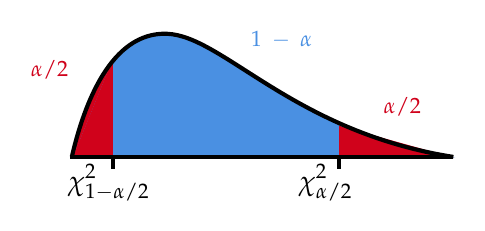
\begin{tikzpicture}[x=0.75pt,y=0.75pt,yscale=-1,xscale=1]
%uncomment if require: \path (0,300); %set diagram left start at 0, and has height of 300

%Curve Lines [id:da6253759692396421] 
\draw [draw opacity=0][fill={rgb, 255:red, 74; green, 144; blue, 226 }  ,fill opacity=1 ][line width=1.5]    (100.83,100.33) .. controls (106.67,75) and (119.67,40) .. (146.67,41) .. controls (173.67,42) and (207.67,88.33) .. (284.67,100.33) ;
%Straight Lines [id:da9705044831224325] 
\draw [draw opacity=0][fill={rgb, 255:red, 208; green, 2; blue, 27 }  ,fill opacity=1 ]   (119.83,52.67) -- (119.83,99.33) -- (100.83,99.33) ;
%Curve Lines [id:da9090824147972125] 
\draw [draw opacity=0][fill={rgb, 255:red, 208; green, 2; blue, 27 }  ,fill opacity=1 ][line width=2.25]    (100.83,99.33) .. controls (106.67,72) and (114.83,58.67) .. (119.83,52.67) ;

%Straight Lines [id:da8243679921312423] 
\draw [draw opacity=0][fill={rgb, 255:red, 208; green, 2; blue, 27 }  ,fill opacity=1 ]   (228.83,85) -- (228.83,100.33) -- (283.83,100.33) ;
%Curve Lines [id:da07655100443368612] 
\draw [line width=1.5]    (100,100) .. controls (105.83,74.67) and (118.83,39.67) .. (145.83,40.67) .. controls (172.83,41.67) and (206.83,88) .. (283.83,100) ;
%Straight Lines [id:da5824849118650262] 
\draw [line width=1.5]    (119.83,100.33) -- (119.83,105.67) ;
%Straight Lines [id:da7912407501617629] 
\draw [line width=1.5]    (228.83,100.33) -- (228.83,105.67) ;
%Straight Lines [id:da26335370673771696] 
\draw [line width=1.5]    (99,100) -- (283.83,100) ;

% Text Node
\draw (79,52) node [anchor=north west][inner sep=0.75pt]  [font=\footnotesize,color={rgb, 255:red, 208; green, 2; blue, 27 }  ,opacity=1 ] [align=left] {$\displaystyle \alpha /2$};
% Text Node
\draw (249,70) node [anchor=north west][inner sep=0.75pt]  [font=\footnotesize,color={rgb, 255:red, 208; green, 2; blue, 27 }  ,opacity=1 ] [align=left] {$\displaystyle \alpha /2$};
% Text Node
\draw (185,38) node [anchor=north west][inner sep=0.75pt]  [font=\footnotesize,color={rgb, 255:red, 74; green, 144; blue, 226 }  ,opacity=1 ] [align=left] {$\displaystyle 1\ -\ \alpha $};
% Text Node
\draw (96.83,102.33) node [anchor=north west][inner sep=0.75pt]   [align=left] {$\displaystyle \chi ^{2}_{1-\alpha /2}$};
% Text Node
\draw (208,102.33) node [anchor=north west][inner sep=0.75pt]   [align=left] {$\displaystyle \chi ^{2}_{\alpha /2}$};


\end{tikzpicture}
\end{center}

Nous sommes donc confiants à un niveau de 100$(1 - \alpha)$\% que :
\begin{align*}
	\sigma^{2} \in \left[
		\frac{(n - 1)s^{2}_{n}}{\chi^{2}_{\alpha / 2}}, 
		\frac{(n - 1)s^{2}_{n}}{\chi^{2}_{1 - \alpha / 2}}
	\right]
\end{align*}
\end{definitionNOHFILLsub}

\begin{definitionNOHFILLsub}[Intervalle de confiance sur la moyenne ($\sigma^{2}$ connue)]
%%%	https://www.youtube.com/watch?v=KG921rfbTDw&list=PLvxOuBpazmsMdPBRxBTvwLv5Lhuk0tuXh&index=4&t=0s
%%%	https://www.youtube.com/watch?v=-iYDu8flFXQ&list=PLvxOuBpazmsMdPBRxBTvwLv5Lhuk0tuXh&index=3&t=268s
Pour l'échantillon aléatoire $\{X_{1}, X_{2}, \dots, X_{n}\}$ issu d'une distribution normale avec $\mu$ inconnu et $\sigma^{2}$ connue, \lfbox[formula]{$\Pr\left(-z_{\alpha/2} \leq \frac{\bar{x} - \mu}{\sigma/\sqrt{n}} \leq z_{\alpha/2}\right) =	(1 - \alpha)$}.\\
Graphiquement:
\begin{center}


\tikzset{every picture/.style={line width=0.75pt}} %set default line width to 0.75pt        

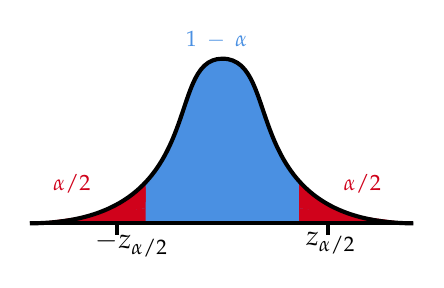
\begin{tikzpicture}[x=0.75pt,y=0.75pt,yscale=-1,xscale=1]
%uncomment if require: \path (0,176); %set diagram left start at 0, and has height of 176

%Curve Lines [id:da8947130044196236] 
\draw [draw opacity=0][fill={rgb, 255:red, 74; green, 144; blue, 226 }  ,fill opacity=1 ][line width=1.5]    (387,99) .. controls (474.83,98.67) and (450.83,19.67) .. (479.83,19.67) .. controls (509.83,19.67) and (485.83,98.67) .. (571.83,99) ;
%Straight Lines [id:da8407133508917781] 
\draw [line width=1.5]    (428.83,99.33) -- (428.83,104.67) ;
%Straight Lines [id:da7153733396293662] 
\draw [line width=1.5]    (530.83,99.33) -- (530.83,104.67) ;
%Straight Lines [id:da1468161753341053] 
\draw [draw opacity=0][fill={rgb, 255:red, 208; green, 2; blue, 27 }  ,fill opacity=1 ]   (516.83,91.67) -- (516.83,99) -- (571.83,99) ;
%Straight Lines [id:da44372694181119354] 
\draw [draw opacity=0][fill={rgb, 255:red, 208; green, 2; blue, 27 }  ,fill opacity=1 ]   (516.83,81.67) -- (516.83,91.67) -- (540.5,95.67) ;
%Straight Lines [id:da871067588661014] 
\draw [draw opacity=0][fill={rgb, 255:red, 208; green, 2; blue, 27 }  ,fill opacity=1 ]   (516.83,78.67) -- (516.83,88.67) -- (528.67,93.67) ;

%Straight Lines [id:da7000317622260974] 
\draw [draw opacity=0][fill={rgb, 255:red, 208; green, 2; blue, 27 }  ,fill opacity=1 ]   (442.83,91.67) -- (442.83,99) -- (387.83,99) ;
%Straight Lines [id:da8176903889743383] 
\draw [draw opacity=0][fill={rgb, 255:red, 208; green, 2; blue, 27 }  ,fill opacity=1 ]   (442.83,81.67) -- (442.83,91.67) -- (419.17,95.67) ;
%Straight Lines [id:da7955659226488763] 
\draw [draw opacity=0][fill={rgb, 255:red, 208; green, 2; blue, 27 }  ,fill opacity=1 ]   (442.83,78.67) -- (442.83,88.67) -- (431,93.67) ;

%Curve Lines [id:da21189166086741196] 
\draw [line width=1.5]    (387,99) .. controls (474.83,98.67) and (450.83,19.67) .. (479.83,19.67) .. controls (509.83,19.67) and (485.83,98.67) .. (571.83,99) ;
%Straight Lines [id:da9615401029487891] 
\draw [line width=1.5]    (387,99) -- (571.83,99) ;


% Text Node
\draw (397,74) node [anchor=north west][inner sep=0.75pt]  [font=\footnotesize,color={rgb, 255:red, 208; green, 2; blue, 27 }  ,opacity=1 ] [align=left] {$\displaystyle \alpha /2$};
% Text Node
\draw (537,74) node [anchor=north west][inner sep=0.75pt]  [font=\footnotesize,color={rgb, 255:red, 208; green, 2; blue, 27 }  ,opacity=1 ] [align=left] {$\displaystyle \alpha /2$};
% Text Node
\draw (461,5) node [anchor=north west][inner sep=0.75pt]  [font=\footnotesize,color={rgb, 255:red, 74; green, 144; blue, 226 }  ,opacity=1 ] [align=left] {$\displaystyle 1\ -\ \alpha $};
% Text Node
\draw (518.83,102) node [anchor=north west][inner sep=0.75pt]   [align=left] {$\displaystyle z_{\alpha /2}$};
% Text Node
\draw (417.33,102) node [anchor=north west][inner sep=0.75pt]   [align=left] {$\displaystyle -z_{\alpha /2}$};


\end{tikzpicture}
\end{center}


Nous sommes donc confiants à un niveau de 100$(1 - \alpha)$\% que :
\begin{equation*}
	\mu \in \left[ \bar{x} - z_{\alpha/2} \frac{\sigma}{\sqrt{n}}, \bar{x} + z_{\alpha/2} \frac{\sigma}{\sqrt{n}}\right].
\end{equation*}
\end{definitionNOHFILLsub}

\begin{definitionNOHFILLsub}[Intervalle de confiance sur la moyenne ($\sigma^{2}$ inconnue)]
Pour l'échantillon aléatoire $\{X_{1}, X_{2}, \dots, X_{n}\}$ issu d'une distribution normale avec $\sigma^{2}$ inconnue, \lfbox[formula]{$\Pr\left(-t_{\alpha/2, n - 1} \leq \frac{\bar{x} - \mu}{s_{n}/\sqrt{n}} \leq t_{\alpha/2, n - 1}\right) =	(1 - \alpha)$}.\\
Graphiquement:
\begin{center}
\tikzset{every picture/.style={line width=0.75pt}} %set default line width to 0.75pt        

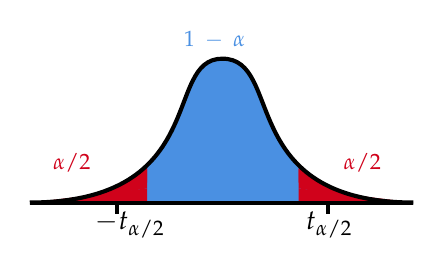
\begin{tikzpicture}[x=0.75pt,y=0.75pt,yscale=-1,xscale=1]
%uncomment if require: \path (0,176); %set diagram left start at 0, and has height of 176

%Curve Lines [id:da982458578172261] 
\draw [draw opacity=0][fill={rgb, 255:red, 74; green, 144; blue, 226 }  ,fill opacity=1 ][line width=1.5]    (386,98) .. controls (473.83,97.67) and (449.83,28.67) .. (478.83,28.67) .. controls (508.83,28.67) and (484.83,97.67) .. (570.83,98) ;
%Straight Lines [id:da3849016484089105] 
\draw [line width=1.5]    (427.83,98.33) -- (427.83,103.67) ;
%Straight Lines [id:da40648686188300065] 
\draw [line width=1.5]    (529.83,98.33) -- (529.83,103.67) ;
%Straight Lines [id:da0901743854683843] 
\draw [draw opacity=0][fill={rgb, 255:red, 208; green, 2; blue, 27 }  ,fill opacity=1 ]   (515.5,91.15) -- (515.5,98) -- (570.83,98) ;
%Straight Lines [id:da7611083055876529] 
\draw [draw opacity=0][fill={rgb, 255:red, 208; green, 2; blue, 27 }  ,fill opacity=1 ]   (515.5,81.8) -- (515.5,91.15) -- (539.31,94.89) ;
%Straight Lines [id:da39003595249115297] 
\draw [draw opacity=0][fill={rgb, 255:red, 208; green, 2; blue, 27 }  ,fill opacity=1 ]   (515.5,79) -- (515.5,88.34) -- (527.41,93.02) ;

%Straight Lines [id:da438403114586448] 
\draw [draw opacity=0][fill={rgb, 255:red, 208; green, 2; blue, 27 }  ,fill opacity=1 ]   (442.5,91.15) -- (442.5,98) -- (386.83,98) ;
%Straight Lines [id:da963730012359405] 
\draw [draw opacity=0][fill={rgb, 255:red, 208; green, 2; blue, 27 }  ,fill opacity=1 ]   (442.5,81.8) -- (442.5,91.15) -- (418.55,94.89) ;
%Straight Lines [id:da7346871172050706] 
\draw [draw opacity=0][fill={rgb, 255:red, 208; green, 2; blue, 27 }  ,fill opacity=1 ]   (442.5,79) -- (442.5,88.34) -- (430.52,93.02) ;

%Curve Lines [id:da971478425929696] 
\draw [line width=1.5]    (386,98) .. controls (473.83,97.67) and (449.83,28.67) .. (478.83,28.67) .. controls (508.83,28.67) and (484.83,97.67) .. (570.83,98) ;
%Straight Lines [id:da9295821978585093] 
\draw [line width=1.5]    (386,98) -- (570.83,98) ;

% Text Node
\draw (396,73) node [anchor=north west][inner sep=0.75pt]  [font=\footnotesize,color={rgb, 255:red, 208; green, 2; blue, 27 }  ,opacity=1 ] [align=left] {$\displaystyle \alpha /2$};
% Text Node
\draw (536,73) node [anchor=north west][inner sep=0.75pt]  [font=\footnotesize,color={rgb, 255:red, 208; green, 2; blue, 27 }  ,opacity=1 ] [align=left] {$\displaystyle \alpha /2$};
% Text Node
\draw (459,14) node [anchor=north west][inner sep=0.75pt]  [font=\footnotesize,color={rgb, 255:red, 74; green, 144; blue, 226 }  ,opacity=1 ] [align=left] {$\displaystyle 1\ -\ \alpha $};
% Text Node
\draw (517.83,101) node [anchor=north west][inner sep=0.75pt]   [align=left] {$\displaystyle t_{\alpha /2}$};
% Text Node
\draw (416.33,101) node [anchor=north west][inner sep=0.75pt]   [align=left] {$\displaystyle -t_{\alpha /2}$};


\end{tikzpicture}
\end{center}

Nous sommes donc confiants à un niveau de 100$(1 - \alpha)$\% que :
\begin{equation*}
	\mu \in \left[ \bar{x} - t_{\alpha/2, n - 1} \frac{s}{\sqrt{n}}, \bar{x} + t_{\alpha/2, n - 1} \frac{s}{\sqrt{n}}\right].
\end{equation*}
\end{definitionNOHFILLsub}


%%%	-------------------------
%%%	NOTES:
%%%	+	À retravailler cette section pour ajouter un peu plus de contexte sur les grands échantillons
%%%	-------------------------


\begin{definitionNOHFILLsub}[Intervalle de confiance \textit{approximatif} sur la moyenne]
%%%	https://www.youtube.com/watch?v=bFefxSE5bmo&list=PLvxOuBpazmsMdPBRxBTvwLv5Lhuk0tuXh&index=8&t=0s
Pour l'échantillon aléatoire $\{X_{1}, X_{2}, \dots, X_{n}\}$ issu d'une distribution avec moyenne $\mu$ et une variance inconnue.\\

Pour $n$ très grand, nous sommes \textit{approximativement} confiants à un niveau de 100$(1 - \alpha)$\% que :
\begin{equation*}
	\mu \in \left[ \bar{x} - z_{\alpha/2} \frac{s}{\sqrt{n}}, \bar{x} + z_{\alpha/2} \frac{s}{\sqrt{n}}\right].
\end{equation*}
\end{definitionNOHFILLsub}

\begin{definitionNOHFILLsub}[Intervalle de confiance \textit{approximatif} sur la proportion]
Pour l'échantillon aléatoire $\{X_{1}, X_{2}, \dots, X_{n}\}$ issu d'une distribution Bernoulli de paramètre $p$.\\

Pour $n$ très grand, nous sommes \textit{approximativement} confiants à un niveau de 100$(1 - \alpha)$\% que :
\begin{equation*}
	p \in \left[ \hat{p} - z_{\alpha/2} \sqrt{\frac{\hat{p}(1 - \hat{p})}{n}}, \hat{p} + z_{\alpha/2} \sqrt{\frac{\hat{p}(1 - \hat{p})}{n}}\right].
\end{equation*}
\end{definitionNOHFILLsub}

On défini le \og \textit{pooled estimator} \fg{} comme la moyenne pondérée des deux variances échantillonnales \lfbox[formula]{$S_{p}^{2}	=	\frac{(n - 1)S_{n}^{2} + (m - 1)S_{m}^{2}}{n + m - 2}$}.\\


\begin{definitionNOHFILLsub}[Intervalle de confiance pour une différence de moyennes]
Pour les échantillons aléatoires $\{X_{1}, X_{2}, \dots, X_{n}\}$ et $\{Y_{1}, Y_{2}, \dots, Y_{m}\}$ issus de distributions normales de moyennes $\mu_{1}$ et $\mu_{2}$ et variance $\sigma^{2}_{1} = \sigma^{2}_{2} = \sigma^{2}$ inconnues.

Nous sommes confiants à un niveau de 100$(1 - \alpha)$\% que :
\begin{equation*}
	(\mu_{1}	-	\mu_{2}) \in \left[ 
	\bar{x}_{n}	-	\bar{y}_{m}
	\pm	t_{\alpha/2, n + m - 2} s_{p}\sqrt{\frac{1}{n} + \frac{1}{m}} \right].
\end{equation*}
\begin{align*}
\end{align*}
\end{definitionNOHFILLsub}

\begin{definitionNOHFILLsub}[Intervalle de confiance \textit{approximatif} pour une différence de moyennes]
Pour les échantillons aléatoires $\{X_{1}, X_{2}, \dots, X_{n}\}$ et $\{Y_{1}, Y_{2}, \dots, Y_{m}\}$ issus de distributions normales de moyennes $\mu_{1}$ et $\mu_{2}$ et variances $\sigma^{2}_{1}$ et $\sigma^{2}_{2}$ inconnues.\\

Pour $n$ très grand, nous sommes \textit{approximativement} confiants à un niveau de 100$(1 - \alpha)$\% que :
\begin{equation*}
	(\mu_{1}	-	\mu_{2}) \in \left[ 
	\bar{x}_{n}	-	\bar{y}_{m}
	\pm	z_{\alpha/2} \sqrt{\frac{s_{n}^{2}}{n} + \frac{s_{m}^{2}}{m}} \right].
\end{equation*}
\begin{align*}
\end{align*}
\end{definitionNOHFILLsub}

\begin{definitionNOHFILLsub}[Intervalle de confiance \textit{approximatif} pour une différence de proportions]
Pour les échantillons aléatoires $\{X_{1}, X_{2}, \dots, X_{n}\}$ et $\{Y_{1}, Y_{2}, \dots, Y_{m}\}$ issus de distributions Bernoulli de paramètres $p_{1}$ et $p_{2}$.\\

Pour $n$ très grand, nous sommes \textit{approximativement} confiants à un niveau de 100$(1 - \alpha)$\% que :
\begin{equation*}
	(p_{1}	-	p_{2}) \in \left[ 
	\hat{p}_{1}	-	\hat{p}_{2}
	\pm	z_{\alpha/2} \sqrt{\frac{\hat{p}_{1}(1 - \hat{p}_{1})}{n} + \frac{\hat{p}_{2}(1 - \hat{p}_{2})}{m}} \right].
\end{equation*}
\begin{align*}
\end{align*}
\end{definitionNOHFILLsub}


%%%
%%%	Méthode du pivot
%%%

\columnbreak
\section{Tests d'hypothèses}
\label{sec:hyp-test}
\subsection{Introduction}
\begin{rappel_enhanced}[Contexte]
Les statistiques classiques posent que tout phénomène observable est régi par un \textit{"\textbf{processus}" sous-jacent}.\\
On ne peut jamais savoir exactement ce qu'est ce "processus"; le mieux que l'on peut faire est d'émettre des \textit{\textbf{hypothèses}} vraisemblables sur ce qu'il pourrait être. \\
Par la suite, on analyse les observations en présumant qu'elles sont régies par le processus hypothétique et détermine la \textit{\textbf{vraisemblance des observations}}. On accepte le processus hypothétique si la vraisemblance est suffisamment élevée.
\end{rappel_enhanced}

\begin{distributions}[Notation]
\begin{description}
	\item[$\Theta_{0}$ et $\Theta_{1}$]	Sous-ensembles disjoints de $\Theta$ tel que \lfbox[formula]{$\Theta_{0} \cup \Theta_{1}	=	\Theta$;}
	\item[$\textrm{H}_{0}$]	Hypothèse nulle ;
		\begin{itemize}
		\item	Représente généralement le statu quo jusqu'à preuve contraire.
		\end{itemize}
	\item[$\textrm{H}_{1}$]	Hypothèse alternative.
		\begin{itemize}
		\item	Représente généralement un changement du statu quo.
		\end{itemize}
\end{description}
\end{distributions}

\begin{definitionNOHFILL}[Test d'hypothèse]
On spécifie une \textcolor{burntorange}{hypothèse} nulle et par conséquent une hypothèse alternative :
\begin{align*}
	\textrm{H}_{0}
	&:	\theta \in \Theta_{0}	&
	&\text{vs}	&
	\textrm{H}_{1}
	&:	\theta \in \Theta_{1}	\\
\end{align*}

Puis, on spécifie une \textcolor{orange-red}{expérience} et un \textcolor{orange}{test} pour décider si l'on accepte ou rejette l'hypothèse nulle.
\end{definitionNOHFILL}

\begin{distributions}[Terminologie]
\begin{description}
\item[Hypothèse simple]	Spécifie \textbf{entièrement} une distribution de probabilité.
	\begin{itemize}
	\item	Par exemple, $\mathcal{H}_{0}	:	q = 0.50$---on connaît la valeur exacte du paramètre $q$ pour une distribution Bernoulli.
	\end{itemize}
\item[Hypothèse composite]	Spécifie \textbf{partiellement} une distribution de probabilité.
	\begin{itemize}
	\item	Par exemple, $\mathcal{H}_{1}	:	q \neq 0.50$.---on ne connaît pas la valeur exacte du paramètre $q$, il pourrait être n'importe quel chiffre sauf $0.50$.
	\end{itemize}
\end{description}
\end{distributions}

\begin{formula}{Exemple du laissez-passer universitaire (LPU)}
\textcolor{orange-red}{Par exemple}, on veut savoir si le monde utilisent l'autobus (oui ou non) avant et après l'implantation du LPU.\\ 
On \textcolor{burntorange}{pose} que la proportion des gens qui utilisent l'autobus est $q	=	0.44$.\\
Il y a deux types de \textcolor{orange}{tests} qu'on peut faire,
\begin{itemize}
	\item	Tester si l'utilisation est différente est un test "\textbf{bilatéral}", car on test si elle a augmentée \textit{ou} diminuée;
		\begin{align*}
		\textrm{H}_{0}
		&:	q	=	0.44	&
		\textrm{H}_{1}
		&:	q	\neq	0.44
		\end{align*}
	\item	Tester si l'utilisation a augmentée est un test "\textbf{unilatéral}", car on test uniquement si elle a augmentée.
		\begin{align*}
		\textrm{H}_{0}
		&:	q	=	0.44	&
		\textrm{H}_{1}
		&:	q	>	0.44
		\end{align*}
\end{itemize}

Un test unilatéral requiert que l'on sache déjà que la proportion de gens "\textit{doit}" être supérieure. Un test bilatéral est plus conservatif et test les deux possibilités, il devrait donc être celui qu'on applique par défaut. \\

L'hypothèse :
\begin{description}
	\item[nulle]		dans les deux cas est que, en moyenne, l'utilisation de l'autobus n'a pas \textit{changée}. 
	\item[alternative]	dans le cas d'un test :
		\begin{description}
		\item[unilatéral]	est que, en moyenne, l'utilisation a \textit{augmentée}.
		\item[bilatéral]	est que, en moyenne, l'utilisation a \textit{changée}.
		\end{description}
\end{description}
\end{formula}

\begin{definitionNOHFILLsub}[Région critique]
\begin{distributions}[Notation]
\begin{description}
	\item[$\mathcal{S}$]	"Ensemble" de tous les résultats possible pour l'échantillon aléatoire;
	\item[$\mathcal{C}$]	\textbf{Région critique} du test qui est un sous-ensemble de $\mathcal{S}$.
\end{description}
\end{distributions}

On rejette $\textrm{H}_{0}$ si $\{X_{1}, \dots, X_{n}\} \in \mathcal{C}$.\\
On conserve $\textrm{H}_{0}$ si $\{X_{1}, \dots, X_{n}\} \in \mathcal{C}^{c}$.

\begin{itemize}
	\item	On peut aussi dire \og \textbf{région de rejet} \fg{}.
\end{itemize}
\end{definitionNOHFILLsub}

\begin{formula}{Exemple du laissez-passer universitaire (LPU)}
On reprend l'exemple du LPU.\\
L'ensemble des résultats possibles est $\mathcal{S} = [0, 1]$.
\begin{itemize}
	\item	Un test "\textbf{bilatéral}" a comme région critique $\mathcal{C} = [0, 0.44) \cup (0.44, 1]$;
	\item	Un test "\textbf{unilatéral}" testant l'augmentation a comme région critique $\mathcal{C} = (0.44, 1]$.
\end{itemize}
\end{formula}

On peut donc faire 2 types d'erreurs:
%%	voir les images que j'ai gardé pour quand je retouche à la matrice de confusion dans les GLMs pour développer et parler des métriques ! 
\begin{center}
\tikzset{every picture/.style={line width=0.75pt}} %set default line width to 0.75pt        

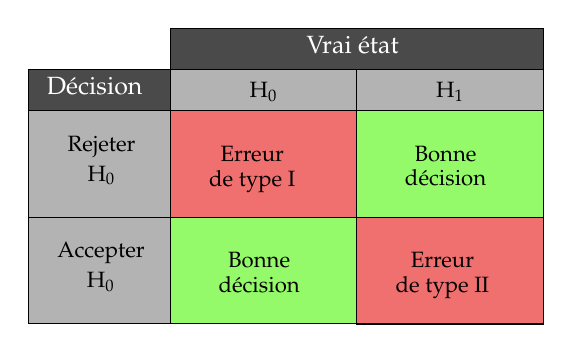
\begin{tikzpicture}[x=0.75pt,y=0.75pt,yscale=-1,xscale=1]
%uncomment if require: \path (0,165); %set diagram left start at 0, and has height of 165

%Shape: Rectangle [id:dp5658804967739193] 
\draw  [fill={rgb, 255:red, 240; green, 111; blue, 111 }  ,fill opacity=1 ] (74,50.17) -- (163.83,50.17) -- (163.83,101.5) -- (74,101.5) -- cycle ;
%Shape: Rectangle [id:dp933461228347003] 
\draw  [fill={rgb, 255:red, 240; green, 111; blue, 111 }  ,fill opacity=1 ] (163.83,101.5) -- (253.67,101.5) -- (253.67,152.83) -- (163.83,152.83) -- cycle ;
%Shape: Rectangle [id:dp24194313951746427] 
\draw  [fill={rgb, 255:red, 148; green, 250; blue, 106 }  ,fill opacity=1 ] (163.83,50) -- (253.67,50) -- (253.67,101.33) -- (163.83,101.33) -- cycle ;
%Shape: Rectangle [id:dp27324261874552724] 
\draw  [fill={rgb, 255:red, 148; green, 250; blue, 106 }  ,fill opacity=1 ] (74,101.33) -- (163.83,101.33) -- (163.83,152.67) -- (74,152.67) -- cycle ;
%Shape: Rectangle [id:dp9425087952138109] 
\draw  [fill={rgb, 255:red, 179; green, 179; blue, 179 }  ,fill opacity=1 ] (74,30.17) -- (163.83,30.17) -- (163.83,50) -- (74,50) -- cycle ;
%Shape: Rectangle [id:dp40513736937576916] 
\draw  [fill={rgb, 255:red, 74; green, 74; blue, 74 }  ,fill opacity=1 ] (74,10.33) -- (253.67,10.33) -- (253.67,30.17) -- (74,30.17) -- cycle ;
%Shape: Rectangle [id:dp4099498200973881] 
\draw  [fill={rgb, 255:red, 179; green, 179; blue, 179 }  ,fill opacity=1 ] (163.83,30.17) -- (253.67,30.17) -- (253.67,50) -- (163.83,50) -- cycle ;
%Shape: Rectangle [id:dp35293578825776084] 
\draw  [fill={rgb, 255:red, 179; green, 179; blue, 179 }  ,fill opacity=1 ] (5.5,101.33) -- (74,101.33) -- (74,152.67) -- (5.5,152.67) -- cycle ;
%Shape: Rectangle [id:dp2841127241620307] 
\draw  [fill={rgb, 255:red, 179; green, 179; blue, 179 }  ,fill opacity=1 ] (5.5,50.17) -- (74,50.17) -- (74,101.5) -- (5.5,101.5) -- cycle ;
%Shape: Rectangle [id:dp5918283025493905] 
\draw  [fill={rgb, 255:red, 74; green, 74; blue, 74 }  ,fill opacity=1 ] (5.5,30.33) -- (74,30.33) -- (74,50.17) -- (5.5,50.17) -- cycle ;

% Text Node
\draw (138.33,13) node [anchor=north west][inner sep=0.75pt]  [font=\small,color={rgb, 255:red, 255; green, 255; blue, 255 }  ,opacity=1 ] [align=left] {Vrai état};
% Text Node
\draw (110.92,35) node [anchor=north west][inner sep=0.75pt]  [font=\footnotesize,color={rgb, 255:red, 0; green, 0; blue, 0 }  ,opacity=1 ] [align=left] {$ \text{H}_{0}$};
% Text Node
\draw (200.75,35) node [anchor=north west][inner sep=0.75pt]  [font=\footnotesize,color={rgb, 255:red, 0; green, 0; blue, 0 }  ,opacity=1 ] [align=left] {$ \text{H}_{1}$};
% Text Node
\draw (18.25,112) node [anchor=north west][inner sep=0.75pt]  [font=\footnotesize,color={rgb, 255:red, 0; green, 0; blue, 0 }  ,opacity=1 ] [align=left] {\shortstack{Accepter\\ $\text{H}_{0}$}};
% Text Node
\draw (23.25,60.83) node [anchor=north west][inner sep=0.75pt]  [font=\footnotesize,color={rgb, 255:red, 0; green, 0; blue, 0 }  ,opacity=1 ] [align=left] {\shortstack{Rejeter\\ $\text{H}_{0}$}};
% Text Node
\draw (13.25,32.75) node [anchor=north west][inner sep=0.75pt]  [font=\small,color={rgb, 255:red, 255; green, 255; blue, 255 }  ,opacity=1 ] [align=left] {Décision};
% Text Node
\draw (91.42,65.83) node [anchor=north west][inner sep=0.75pt]  [font=\footnotesize,color={rgb, 255:red, 0; green, 0; blue, 0 }  ,opacity=1 ] [align=left] 
{\shortstack{Erreur\\ de type I}};
% Text Node
\draw (181.25,117) node [anchor=north west][inner sep=0.75pt]  [font=\footnotesize,color={rgb, 255:red, 0; green, 0; blue, 0 }  ,opacity=1 ] [align=left] {\shortstack{Erreur\\ de type II}};
% Text Node
\draw (95.92,117) node [anchor=north west][inner sep=0.75pt]  [font=\footnotesize,color={rgb, 255:red, 0; green, 0; blue, 0 }  ,opacity=1 ] [align=left] {\shortstack{Bonne\\ décision}};
% Text Node
\draw (185.75,65.67) node [anchor=north west][inner sep=0.75pt]  [font=\footnotesize,color={rgb, 255:red, 0; green, 0; blue, 0 }  ,opacity=1 ] [align=left] {\shortstack{Bonne\\ décision}};



\end{tikzpicture}
\end{center}

\columnbreak
\subsection{Certitude du test}
Lorsque nous voulons quantifier le degré auquel nous sommes confiants du test, nous utilisons la valeur $p$. \\
La valeur $p$ a trois composantes:
\begin{enumerate}
	\item	La probabilité que l'événement se produise aléatoirement.
	\item	La probabilité qu'un événement tout aussi rare se produise.
	\item	La probabilité qu'un événement encore plus rare se produise.
\end{enumerate}

\begin{formula}{Exemple de pile ou face}
On souhaite tester si, en obtenant deux piles sur deux lancers, nous avons une pièce de monnaie truquée :
\begin{description}
	\item[Hypothèse nulle]	Ma pièce de monnaie n'est pas truquée même si j'ai obtenu deux piles.
\end{description}
\

Étapes du calcul de la valeur $p$:
\begin{enumerate}
	\item	On calcule la probabilité d'obtenir 2 piles: $0.5 \times 0.5 = 0.25$.
	\item	Puis, on calcule la probabilité d'obtenir 2 faces (un événement autant rare): $0.5 \times 0.5 = 0.25$.
	\item	Finalement, il n'y a pas d'autres séquences plus rares.
\end{enumerate}
Donc, la valeur $p$ du test est de $0.50$.

\begin{itemize}
	\item	Ceci est plutôt élevé;
	\item	Souvent, on pose que la valeur $p$ du test doit être d'au plus $0.05$;
	\item	Ce qui veut dire que des événements tout aussi (ou plus) rares doivent arriver moins que 5\% du temps pour que l'on considère la pièce de monnaie comme étant truquée;
	\item	Donc, dans notre cas, on ne peut pas rejeter l'hypothèse nulle que notre pièce de monnaie n'est pas spéciale.
\end{itemize}
\end{formula}

Dans le cas continu, on somme les probabilités d'être plus rare ou d'être moins rare. C'est la même idée que les intervalles de confiance avec la valeur $p$, ou \textit{seuil de signifiance $\alpha$}, représenté en rouge. 
\begin{itemize}
	\item	Si la valeur $p$ est petite, ceci indique que d'autres distributions pourraient potentiellement mieux s'ajuster aux données puisque l'événement est très rare;
	\item	Si la valeur $p$ est grande, ceci indique que l'événement est très courant et que la distribution semble être bien ajustée.
\end{itemize}

\

Il y a plusieurs termes semblables qui peuvent devenir mélangeants.
\begin{distributions}[Terminologie]
\begin{description}
	\item[$p$]	La \textbf{valeur $p$} du test.
		\begin{itemize}
		\item	On peut la définir comme la probabilité d'un événement autant (ou plus) rare sous l'hypothèse nulle ;
		\item	On peut la définir comme la \textbf{taille} de la région critique $\mathcal{C}$ ; c'est-à-dire, l'\textit{aire} de la région de rejet de l'hypothèse nulle $\text{H}_{0}$ alors qu'elle est vraie ;
		\item	On peut la définir comme le \textbf{seuil de signifiance} ; c'est-à-dire, la probabilité de rejeter $\text{H}_{0}$ alors qu'elle est vraie ;
		\item	Elle correspond donc également à la \textbf{probabilité d'une erreur de type I}.
		\end{itemize}
	\item[$\alpha$]	Dénote habituellement le \textbf{seuil de signifiance} ou la \textbf{taille} du test.
		\begin{itemize}
		\item	Même idée qu'avec les intervalles de confiance;
		\item	On peut parfois aussi utiliser $\alpha$ pour dénoter la valeur de $p$ qui détermine si on rejette ou pas un test ;
		\item	En anglais, \og \textit{threshold for significance} \fg{}.
		\end{itemize}
\end{description}
\end{distributions}

Formellement, on défini \lfbox[formula]{$\alpha	=	{\color{indigo(web)}\max}_{{\color{amethyst}\theta} \in {\color{pastelred}\Theta_{0}}} \Pr\left\{{\color{bondiblue!80!black}(X_{1}, \dots, X_{n})} {\color{armygreen}\in} {\color{bulgarianrose}\mathcal{C}} ; {\color{amethyst}\theta} \right\}$}. \\
C'est-à-dire :
\begin{itemize}
	\item	on \textcolor{indigo(web)}{maximise} la probabilité que \textcolor{bondiblue!80!black}{l'échantillon aléatoire} soit \textcolor{armygreen}{contenu} dans \textcolor{bulgarianrose!90!black}{la région critique} (alias rejeter $\textrm{H}_{0}$), 
	\item	où la distribution est tracée \textcolor{amethyst}{en fonction du paramètre $\theta$} de \textcolor{pastelred}{l'hypothèse nulle}.
\end{itemize}


\columnbreak
\subsection{Puissance d'un test}
\begin{definitionNOHFILL}[La puissance d'un test]
La probabilité de \textit{correctement} rejeter l'hypothèse nulle.
%%	https://www.youtube.com/watch?v=Rsc5znwR5FA&feature=youtu.be

\tcbline

Une analyse de la puissance détermine le nombre d'observations qu'il faut afin d'avoir une probabilité élevée de correctement rejeter l'hypothèse nulle.
\end{definitionNOHFILL}


Plusieurs facteurs influencent la puissance d'un test. Lorsqu'on teste si deux échantillons d'observations proviennent de la même distribution,
\begin{definitionNOHFILLsub}[La forme de la distribution]
Si les deux distributions sont:
\begin{itemize}
	\item	Très \textbf{distinctes}, la puissance sera très \textbf{élevée}:
		\begin{center}
		\tikzset{every picture/.style={line width=0.75pt}} %set default line width to 0.75pt        

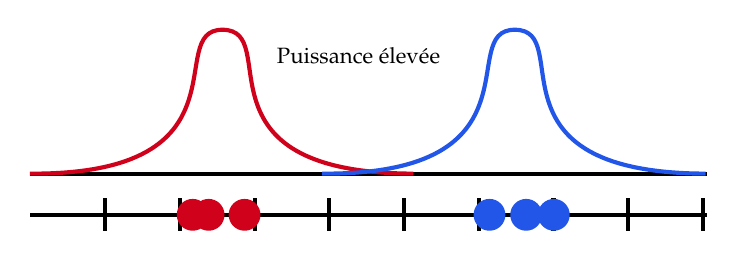
\begin{tikzpicture}[x=0.75pt,y=0.75pt,yscale=-1,xscale=1]
%uncomment if require: \path (0,176); %set diagram left start at 0, and has height of 176

%Straight Lines [id:da864976542619565] 
\draw [line width=1.5]    (245.5,117.83) -- (571.5,117.83) (281.5,109.83) -- (281.5,125.83)(317.5,109.83) -- (317.5,125.83)(353.5,109.83) -- (353.5,125.83)(389.5,109.83) -- (389.5,125.83)(425.5,109.83) -- (425.5,125.83)(461.5,109.83) -- (461.5,125.83)(497.5,109.83) -- (497.5,125.83)(533.5,109.83) -- (533.5,125.83)(569.5,109.83) -- (569.5,125.83) ;
%Straight Lines [id:da9295821978585093] 
\draw [line width=1.5]    (245.17,98) -- (571.5,98) ;
%Curve Lines [id:da28384300225010417] 
\draw [color={rgb, 255:red, 208; green, 2; blue, 27 }  ,draw opacity=1 ][line width=1.5]    (245.17,98) .. controls (353.67,98.67) and (309,28.67) .. (338,28.67) .. controls (368,28.67) and (320.67,97.67) .. (430,98) ;
%Curve Lines [id:da19190888762749303] 
\draw [color={rgb, 255:red, 33; green, 86; blue, 233 }  ,draw opacity=1 ][line width=1.5]    (386,98) .. controls (494.5,98.67) and (449.83,28.67) .. (478.83,28.67) .. controls (508.83,28.67) and (461.5,97.67) .. (570.83,98) ;
%Shape: Circle [id:dp23295532013997544] 
\draw  [draw opacity=0][fill={rgb, 255:red, 208; green, 2; blue, 27 }  ,fill opacity=1 ] (316,117.83) .. controls (316,113.6) and (319.43,110.17) .. (323.67,110.17) .. controls (327.9,110.17) and (331.33,113.6) .. (331.33,117.83) .. controls (331.33,122.07) and (327.9,125.5) .. (323.67,125.5) .. controls (319.43,125.5) and (316,122.07) .. (316,117.83) -- cycle ;
%Shape: Circle [id:dp6583442494748755] 
\draw  [draw opacity=0][fill={rgb, 255:red, 208; green, 2; blue, 27 }  ,fill opacity=1 ] (323.67,117.83) .. controls (323.67,113.6) and (327.1,110.17) .. (331.33,110.17) .. controls (335.57,110.17) and (339,113.6) .. (339,117.83) .. controls (339,122.07) and (335.57,125.5) .. (331.33,125.5) .. controls (327.1,125.5) and (323.67,122.07) .. (323.67,117.83) -- cycle ;
%Shape: Circle [id:dp7278683126625956] 
\draw  [draw opacity=0][fill={rgb, 255:red, 208; green, 2; blue, 27 }  ,fill opacity=1 ] (341,117.83) .. controls (341,113.6) and (344.43,110.17) .. (348.67,110.17) .. controls (352.9,110.17) and (356.33,113.6) .. (356.33,117.83) .. controls (356.33,122.07) and (352.9,125.5) .. (348.67,125.5) .. controls (344.43,125.5) and (341,122.07) .. (341,117.83) -- cycle ;
%Shape: Circle [id:dp6846096733160589] 
\draw  [draw opacity=0][fill={rgb, 255:red, 33; green, 86; blue, 233 }  ,fill opacity=1 ] (459,117.83) .. controls (459,113.6) and (462.43,110.17) .. (466.67,110.17) .. controls (470.9,110.17) and (474.33,113.6) .. (474.33,117.83) .. controls (474.33,122.07) and (470.9,125.5) .. (466.67,125.5) .. controls (462.43,125.5) and (459,122.07) .. (459,117.83) -- cycle ;
%Shape: Circle [id:dp05843938160550621] 
\draw  [draw opacity=0][fill={rgb, 255:red, 33; green, 86; blue, 233 }  ,fill opacity=1 ] (476.67,117.83) .. controls (476.67,113.6) and (480.1,110.17) .. (484.33,110.17) .. controls (488.57,110.17) and (492,113.6) .. (492,117.83) .. controls (492,122.07) and (488.57,125.5) .. (484.33,125.5) .. controls (480.1,125.5) and (476.67,122.07) .. (476.67,117.83) -- cycle ;
%Shape: Circle [id:dp2540684792866683] 
\draw  [draw opacity=0][fill={rgb, 255:red, 33; green, 86; blue, 233 }  ,fill opacity=1 ] (490,117.83) .. controls (490,113.6) and (493.43,110.17) .. (497.67,110.17) .. controls (501.9,110.17) and (505.33,113.6) .. (505.33,117.83) .. controls (505.33,122.07) and (501.9,125.5) .. (497.67,125.5) .. controls (493.43,125.5) and (490,122.07) .. (490,117.83) -- cycle ;

% Text Node
\draw (363,36) node [anchor=north west][inner sep=0.75pt]  [font=\footnotesize,color={rgb, 255:red, 255; green, 255; blue, 255 }  ,opacity=1 ] [align=left] {\textcolor{black}{Puissance élevée}};


\end{tikzpicture}
		\end{center}
		\begin{itemize}
		\item	 La probabilité de \textbf{correctement} rejeter l'hypothèse nulle (que les deux échantillons proviennent d'une même distribution) est élevée;
		\item	On peut aussi dire qu'il y a une forte probabilité de \textbf{correctement} obtenir une faible valeur $p$.
		\end{itemize}
	\item	Se \textbf{chevauchent}, la puissance sera \textbf{faible}:
		\begin{center}
		\tikzset{every picture/.style={line width=0.75pt}} %set default line width to 0.75pt        

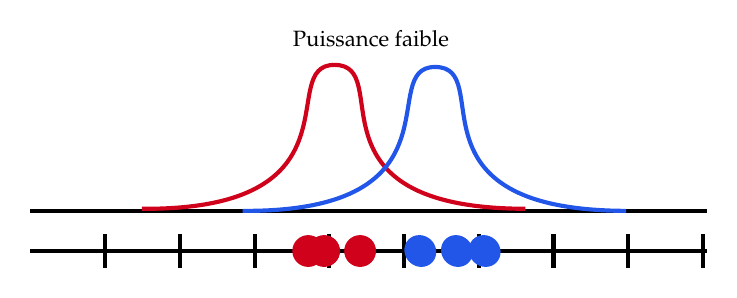
\begin{tikzpicture}[x=0.75pt,y=0.75pt,yscale=-1,xscale=1]
%uncomment if require: \path (0,176); %set diagram left start at 0, and has height of 176

%Straight Lines [id:da674545395459474] 
\draw [line width=1.5]    (244.83,117.33) -- (570.83,117.33) (280.83,109.33) -- (280.83,125.33)(316.83,109.33) -- (316.83,125.33)(352.83,109.33) -- (352.83,125.33)(388.83,109.33) -- (388.83,125.33)(424.83,109.33) -- (424.83,125.33)(460.83,109.33) -- (460.83,125.33)(496.83,109.33) -- (496.83,125.33)(532.83,109.33) -- (532.83,125.33)(568.83,109.33) -- (568.83,125.33) ;
%Shape: Circle [id:dp5899062048279418] 
\draw  [draw opacity=0][fill={rgb, 255:red, 208; green, 2; blue, 27 }  ,fill opacity=1 ] (371,117.33) .. controls (371,113.1) and (374.43,109.67) .. (378.67,109.67) .. controls (382.9,109.67) and (386.33,113.1) .. (386.33,117.33) .. controls (386.33,121.57) and (382.9,125) .. (378.67,125) .. controls (374.43,125) and (371,121.57) .. (371,117.33) -- cycle ;
%Shape: Circle [id:dp033764139219446765] 
\draw  [draw opacity=0][fill={rgb, 255:red, 208; green, 2; blue, 27 }  ,fill opacity=1 ] (378.67,117.33) .. controls (378.67,113.1) and (382.1,109.67) .. (386.33,109.67) .. controls (390.57,109.67) and (394,113.1) .. (394,117.33) .. controls (394,121.57) and (390.57,125) .. (386.33,125) .. controls (382.1,125) and (378.67,121.57) .. (378.67,117.33) -- cycle ;
%Shape: Circle [id:dp9956436610120569] 
\draw  [draw opacity=0][fill={rgb, 255:red, 208; green, 2; blue, 27 }  ,fill opacity=1 ] (396,117.33) .. controls (396,113.1) and (399.43,109.67) .. (403.67,109.67) .. controls (407.9,109.67) and (411.33,113.1) .. (411.33,117.33) .. controls (411.33,121.57) and (407.9,125) .. (403.67,125) .. controls (399.43,125) and (396,121.57) .. (396,117.33) -- cycle ;
%Straight Lines [id:da9463171904376761] 
\draw [line width=1.5]    (244.5,98) -- (570.83,98) ;
%Curve Lines [id:da7529446506143549] 
\draw [color={rgb, 255:red, 208; green, 2; blue, 27 }  ,draw opacity=1 ][line width=1.5]    (298.5,97) .. controls (407,97.67) and (362.33,27.67) .. (391.33,27.67) .. controls (421.33,27.67) and (374,96.67) .. (483.33,97) ;
%Curve Lines [id:da7479872172646262] 
\draw [color={rgb, 255:red, 33; green, 86; blue, 233 }  ,draw opacity=1 ][line width=1.5]    (347,98) .. controls (455.5,98.67) and (410.83,28.67) .. (439.83,28.67) .. controls (469.83,28.67) and (422.5,97.67) .. (531.83,98) ;
%Shape: Circle [id:dp8825558203269679] 
\draw  [draw opacity=0][fill={rgb, 255:red, 33; green, 86; blue, 233 }  ,fill opacity=1 ] (425,117.33) .. controls (424.72,113.1) and (427.93,109.67) .. (432.17,109.67) .. controls (436.4,109.67) and (440.06,113.1) .. (440.33,117.33) .. controls (440.61,121.57) and (437.4,125) .. (433.17,125) .. controls (428.93,125) and (425.28,121.57) .. (425,117.33) -- cycle ;
%Shape: Circle [id:dp2808249488586654] 
\draw  [draw opacity=0][fill={rgb, 255:red, 33; green, 86; blue, 233 }  ,fill opacity=1 ] (442.67,117.33) .. controls (442.39,113.1) and (445.6,109.67) .. (449.83,109.67) .. controls (454.07,109.67) and (457.72,113.1) .. (458,117.33) .. controls (458.28,121.57) and (455.07,125) .. (450.83,125) .. controls (446.6,125) and (442.94,121.57) .. (442.67,117.33) -- cycle ;
%Shape: Circle [id:dp8643138982751464] 
\draw  [draw opacity=0][fill={rgb, 255:red, 33; green, 86; blue, 233 }  ,fill opacity=1 ] (456,117.33) .. controls (455.72,113.1) and (458.93,109.67) .. (463.17,109.67) .. controls (467.4,109.67) and (471.06,113.1) .. (471.33,117.33) .. controls (471.61,121.57) and (468.4,125) .. (464.17,125) .. controls (459.93,125) and (456.28,121.57) .. (456,117.33) -- cycle ;

% Text Node
\draw (370,10) node [anchor=north west][inner sep=0.75pt]  [font=\footnotesize,color={rgb, 255:red, 255; green, 255; blue, 255 }  ,opacity=1 ] [align=left] {\textcolor{black}{Puissance faible}};


\end{tikzpicture}
		\end{center}
		\begin{itemize}
		\item	 La probabilité de \textbf{incorrectement} rejeter l'hypothèse nulle (que les deux échantillons proviennent d'une même distribution) est élevée;
		\item	On peut aussi dire qu'il y a une forte probabilité de \textbf{incorrectement} obtenir une faible valeur $p$;
		\item	Cependant, la puissance peut être augmentée avec plus d'observations.
		\end{itemize}
\end{itemize}
\end{definitionNOHFILLsub}

\begin{definitionNOHFILLsub}[La variabilité des données]
Si la variabilité de la distribution est
\begin{itemize}
	\item	\textbf{Faible}, alors la variabilité de l'échantillon sera probablement faible aussi menant à une puissance très \textbf{élevée}:
		\begin{center}
		\tikzset{every picture/.style={line width=0.75pt}} %set default line width to 0.75pt        

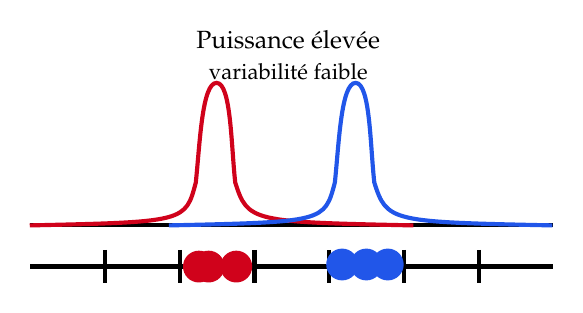
\begin{tikzpicture}[x=0.75pt,y=0.75pt,yscale=-1,xscale=1]
%uncomment if require: \path (0,176); %set diagram left start at 0, and has height of 176

%Straight Lines [id:da864976542619565] 
\draw [line width=1.5]    (245.42,117.83) -- (497.17,117.83) (281.42,109.83) -- (281.42,125.83)(317.42,109.83) -- (317.42,125.83)(353.42,109.83) -- (353.42,125.83)(389.42,109.83) -- (389.42,125.83)(425.42,109.83) -- (425.42,125.83)(461.42,109.83) -- (461.42,125.83) ;
%Straight Lines [id:da9295821978585093] 
\draw [line width=1.5]    (245.17,98) -- (497.17,98) ;
%Shape: Circle [id:dp23295532013997544] 
\draw  [draw opacity=0][fill={rgb, 255:red, 208; green, 2; blue, 27 }  ,fill opacity=1 ] (319,117.83) .. controls (319,113.6) and (322.43,110.17) .. (326.67,110.17) .. controls (330.9,110.17) and (334.33,113.6) .. (334.33,117.83) .. controls (334.33,122.07) and (330.9,125.5) .. (326.67,125.5) .. controls (322.43,125.5) and (319,122.07) .. (319,117.83) -- cycle ;
%Shape: Circle [id:dp6583442494748755] 
\draw  [draw opacity=0][fill={rgb, 255:red, 208; green, 2; blue, 27 }  ,fill opacity=1 ] (323.67,117.83) .. controls (323.67,113.6) and (327.1,110.17) .. (331.33,110.17) .. controls (335.57,110.17) and (339,113.6) .. (339,117.83) .. controls (339,122.07) and (335.57,125.5) .. (331.33,125.5) .. controls (327.1,125.5) and (323.67,122.07) .. (323.67,117.83) -- cycle ;
%Shape: Circle [id:dp7278683126625956] 
\draw  [draw opacity=0][fill={rgb, 255:red, 208; green, 2; blue, 27 }  ,fill opacity=1 ] (337,117.83) .. controls (337,113.6) and (340.43,110.17) .. (344.67,110.17) .. controls (348.9,110.17) and (352.33,113.6) .. (352.33,117.83) .. controls (352.33,122.07) and (348.9,125.5) .. (344.67,125.5) .. controls (340.43,125.5) and (337,122.07) .. (337,117.83) -- cycle ;
%Shape: Circle [id:dp6846096733160589] 
\draw  [draw opacity=0][fill={rgb, 255:red, 33; green, 86; blue, 233 }  ,fill opacity=1 ] (388,116.83) .. controls (388,112.6) and (391.43,109.17) .. (395.67,109.17) .. controls (399.9,109.17) and (403.33,112.6) .. (403.33,116.83) .. controls (403.33,121.07) and (399.9,124.5) .. (395.67,124.5) .. controls (391.43,124.5) and (388,121.07) .. (388,116.83) -- cycle ;
%Shape: Circle [id:dp05843938160550621] 
\draw  [draw opacity=0][fill={rgb, 255:red, 33; green, 86; blue, 233 }  ,fill opacity=1 ] (399.67,116.83) .. controls (399.67,112.6) and (403.1,109.17) .. (407.33,109.17) .. controls (411.57,109.17) and (415,112.6) .. (415,116.83) .. controls (415,121.07) and (411.57,124.5) .. (407.33,124.5) .. controls (403.1,124.5) and (399.67,121.07) .. (399.67,116.83) -- cycle ;
%Shape: Circle [id:dp2540684792866683] 
\draw  [draw opacity=0][fill={rgb, 255:red, 33; green, 86; blue, 233 }  ,fill opacity=1 ] (410,116.83) .. controls (410,112.6) and (413.43,109.17) .. (417.67,109.17) .. controls (421.9,109.17) and (425.33,112.6) .. (425.33,116.83) .. controls (425.33,121.07) and (421.9,124.5) .. (417.67,124.5) .. controls (413.43,124.5) and (410,121.07) .. (410,116.83) -- cycle ;
%Curve Lines [id:da9834393207352259] 
\draw [color={rgb, 255:red, 208; green, 2; blue, 27 }  ,draw opacity=1 ][line width=1.5]    (245.17,98) .. controls (320.17,96.33) and (320.17,96.33) .. (325.17,77.33) .. controls (327.17,58.33) and (328.17,29.33) .. (335.17,29.33) .. controls (342.17,29.33) and (342.17,59.33) .. (344.17,77.33) .. controls (350.17,96.33) and (352.17,96.33) .. (430,98) ;
%Curve Lines [id:da5775597107131041] 
\draw [color={rgb, 255:red, 33; green, 86; blue, 233 }  ,draw opacity=1 ][line width=1.5]    (312.17,98) .. controls (387.17,96.33) and (387.17,96.33) .. (392.17,77.33) .. controls (394.17,58.33) and (395.17,29.33) .. (402.17,29.33) .. controls (409.17,29.33) and (409.17,59.33) .. (411.17,77.33) .. controls (417.17,96.33) and (419.17,96.33) .. (497,98) ;

% Text Node
\draw (324,3) node [anchor=north west][inner sep=0.75pt]  [font=\small,color={rgb, 255:red, 0; green, 0; blue, 0 }  ,opacity=1 ] [align=left] {\begin{minipage}[lt]{66.6825pt}\setlength\topsep{0pt}
\begin{center}
Puissance élevée\\{\footnotesize variabilité faible}
\end{center}

\end{minipage}};


\end{tikzpicture}
		\end{center}
	\item	\textbf{Élevée}, alors la variabilité de l'échantillon sera probablement élevée aussi menant à une puissance \textbf{faible}: 
		\begin{center}
		\tikzset{every picture/.style={line width=0.75pt}} %set default line width to 0.75pt        

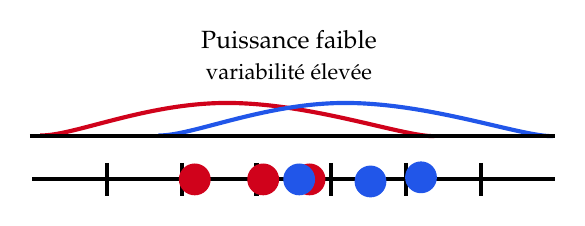
\begin{tikzpicture}[x=0.75pt,y=0.75pt,yscale=-1,xscale=1]
%uncomment if require: \path (0,176); %set diagram left start at 0, and has height of 176

%Straight Lines [id:da224342647816256] 
\draw [line width=1.5]    (291.42,122.83) -- (543.17,122.83) (327.42,114.83) -- (327.42,130.83)(363.42,114.83) -- (363.42,130.83)(399.42,114.83) -- (399.42,130.83)(435.42,114.83) -- (435.42,130.83)(471.42,114.83) -- (471.42,130.83)(507.42,114.83) -- (507.42,130.83) ;
%Shape: Circle [id:dp7289237376471596] 
\draw  [draw opacity=0][fill={rgb, 255:red, 208; green, 2; blue, 27 }  ,fill opacity=1 ] (362,122.83) .. controls (362,118.6) and (365.43,115.17) .. (369.67,115.17) .. controls (373.9,115.17) and (377.33,118.6) .. (377.33,122.83) .. controls (377.33,127.07) and (373.9,130.5) .. (369.67,130.5) .. controls (365.43,130.5) and (362,127.07) .. (362,122.83) -- cycle ;
%Shape: Circle [id:dp6581028616853248] 
\draw  [draw opacity=0][fill={rgb, 255:red, 208; green, 2; blue, 27 }  ,fill opacity=1 ] (417.3,122.83) .. controls (417.3,118.6) and (420.73,115.17) .. (424.96,115.17) .. controls (429.2,115.17) and (432.63,118.6) .. (432.63,122.83) .. controls (432.63,127.07) and (429.2,130.5) .. (424.96,130.5) .. controls (420.73,130.5) and (417.3,127.07) .. (417.3,122.83) -- cycle ;
%Shape: Circle [id:dp32832339728857773] 
\draw  [draw opacity=0][fill={rgb, 255:red, 208; green, 2; blue, 27 }  ,fill opacity=1 ] (394.96,122.83) .. controls (394.96,118.6) and (398.39,115.17) .. (402.63,115.17) .. controls (406.86,115.17) and (410.3,118.6) .. (410.3,122.83) .. controls (410.3,127.07) and (406.86,130.5) .. (402.63,130.5) .. controls (398.39,130.5) and (394.96,127.07) .. (394.96,122.83) -- cycle ;
%Shape: Circle [id:dp8463878803176157] 
\draw  [draw opacity=0][fill={rgb, 255:red, 33; green, 86; blue, 233 }  ,fill opacity=1 ] (412.3,122.83) .. controls (412.3,118.6) and (415.73,115.17) .. (419.96,115.17) .. controls (424.2,115.17) and (427.63,118.6) .. (427.63,122.83) .. controls (427.63,127.07) and (424.2,130.5) .. (419.96,130.5) .. controls (415.73,130.5) and (412.3,127.07) .. (412.3,122.83) -- cycle ;
%Shape: Circle [id:dp41576741952688256] 
\draw  [draw opacity=0][fill={rgb, 255:red, 33; green, 86; blue, 233 }  ,fill opacity=1 ] (446.67,123.83) .. controls (446.67,119.6) and (450.1,116.17) .. (454.33,116.17) .. controls (458.57,116.17) and (462,119.6) .. (462,123.83) .. controls (462,128.07) and (458.57,131.5) .. (454.33,131.5) .. controls (450.1,131.5) and (446.67,128.07) .. (446.67,123.83) -- cycle ;
%Shape: Circle [id:dp7322447345202854] 
\draw  [draw opacity=0][fill={rgb, 255:red, 33; green, 86; blue, 233 }  ,fill opacity=1 ] (471,121.83) .. controls (471,117.6) and (474.43,114.17) .. (478.67,114.17) .. controls (482.9,114.17) and (486.33,117.6) .. (486.33,121.83) .. controls (486.33,126.07) and (482.9,129.5) .. (478.67,129.5) .. controls (474.43,129.5) and (471,126.07) .. (471,121.83) -- cycle ;
%Curve Lines [id:da3201541308920388] 
\draw [color={rgb, 255:red, 208; green, 2; blue, 27 }  ,draw opacity=1 ][line width=1.5]    (295.17,101.67) .. controls (311.17,102) and (346.17,86) .. (385.17,86) .. controls (426.17,86) and (470.33,102.33) .. (485.17,102) ;
%Curve Lines [id:da0520324915772159] 
\draw [color={rgb, 255:red, 33; green, 86; blue, 233 }  ,draw opacity=1 ][line width=1.5]    (352.17,101.67) .. controls (368.17,102) and (403.17,86) .. (442.17,86) .. controls (483.17,86) and (527.33,102.33) .. (542.17,102) ;
%Straight Lines [id:da9874290431386423] 
\draw [line width=1.5]    (290.17,102) -- (543.17,102) ;

% Text Node
\draw (371,50) node [anchor=north west][inner sep=0.75pt]  [font=\small,color={rgb, 255:red, 0; green, 0; blue, 0 }  ,opacity=1 ] [align=left] {\begin{minipage}[lt]{64.149144pt}\setlength\topsep{0pt}
\begin{center}
Puissance faible\\{\footnotesize variabilité élevée}
\end{center}

\end{minipage}};
\end{tikzpicture}
		\end{center}
\end{itemize}
\end{definitionNOHFILLsub}

Il existe plusieurs mesures qui permettent de considérer la variabilité des données ainsi que la forme de la distribution. Entres autre, il y a le \og \textit{\textbf{effect size ($d$)}} \fg{} où \lfbox[formula]{$d	=	\frac{\bar{x} - \bar{y}}{s^{2}_{p}}$}.

\begin{definitionNOHFILLsub}[Le taille de l'échantillon de données]
Un grand échantillon de données peut compenser pour des distributions qui se chevauchent ou une variabilité élevée. Ça permet d'augmenter notre \textit{confiance} qu'il y a bel et bien une différence entre les échantillons. \\

En contraste, nous n'avons pas besoin d'un grand échantillon de données pour des distributions très distinctes ou avec une faible variabilité; nous sommes déjà confiants que les distributions sont différentes.
\end{definitionNOHFILLsub}

\begin{definitionNOHFILLsub}[Le test statistique]
Certains tests ont une puissance plus élevée que les autres. \\
Cela dit, le test $t$ habituel est très puissant.
\end{definitionNOHFILLsub}

\subsubsection{La fonction de puissance}

La fonction de puissance est \lfbox[formula]{$\gamma(\theta)	=	\Pr\left\{(X_{1}, \dots, X_{n}) \in \mathcal{C} ; \theta \right\}$} ; c'est-à-dire, la probabilité de rejeter l'hypothèse nulle $\mathrm{H}_{0}$ si la \textbf{vraie} valeur du paramètre est $\theta \in \Theta$. 
\begin{itemize}
	\item	C'est une fonction de $\theta$ ;
	\item	Idéalement, si l'hypothèse nulle est :
		\begin{description}
		\item[acceptée]	on souhaite que $\gamma(\theta)	=	0$ puisque $\theta \in \Theta_{0}$.
			\begin{itemize}
			\item	On dénote $\gamma(\theta_{0})	=	\Pr\left\{(X_{1}, \dots, X_{n}) \in \mathcal{C} ;  \theta \in \Theta_{0}\right\}	=	0$.
			\end{itemize}
		\item[rejetée]	on souhaite que $\gamma(\theta)	=	1$ puisque $\theta \in \Theta_{1}$.
			\begin{itemize}
			\item	On dénote $\gamma(\theta_{1})	=	\Pr\left\{(X_{1}, \dots, X_{n}) \in \mathcal{C} ; \theta \in \Theta_{1}\right\}	=	1$.
			\end{itemize}
		\end{description}
\end{itemize}

Si, par exemple, on rejette l'hypothèse nulle on pourrait tracer la fonction de puissance pour toutes les valeurs possibles de l'ensemble $\Theta_{1}$.


%%	
%	\lfbox[formula]{$n \geq \left(\frac{z}{k - \mu_{1}}\right)^{2}\sigma^{2}$}.


\columnbreak

\subsection{Tests optimaux}
\begin{distributions}[Notation]
\begin{description}
	\item[$\delta$]	(Procédure de) test ;
	\item[$\alpha(\delta)$]	Probabilité d'une erreur de type I pour un test $\delta$ ;
		\begin{itemize}
		\item	$\alpha(\delta)	=	\Pr\left\{(X_{1}, \dots, X_{n}) \in \mathcal{C} ;  \theta \in \Theta_{0}\right\}	=	\gamma(\theta_{0})$.
		\end{itemize}
	\item[$\beta(\delta)$]	Probabilité d'une erreur de type II pour un test $\delta$ ;
		\begin{itemize}
		\item	$\beta(\delta)	=	\Pr\left\{(X_{1}, \dots, X_{n}) \in \mathcal{C}^{\complement} ;  \theta \in \Theta_{1}\right\}	=	1 - \gamma(\theta_{1})$.
		\end{itemize}
\end{description}
\end{distributions}

\begin{definitionNOHFILLprop}[Tests optimaux]
Bien qu'il est impossible de trouver un test $\delta$ pour lequel les probabilités d'erreurs de type I et II sont très petites, on peut minimiser $a\alpha(\delta) + b\beta(\delta)$.

\tcbline

Soit les constantes $a, b > 0$.\\
Soit un test $\delta^{*}$ tel que :
\begin{itemize}
	\item	 $\mathrm{H}_{0}$ est acceptée si \lfbox[conditions]{$af(\bm{x} ; \theta_{0})	>	bf(\bm{x} ; \theta_{1})$} ;
	\item	 $\mathrm{H}_{0}$ est rejetée si \lfbox[conditions]{$af(\bm{x} ; \theta_{0})	<	bf(\bm{x} ; \theta_{1})$} ;
	\item	Si \lfbox[conditions]{$af(\bm{x} ; \theta_{0})	=	bf(\bm{x} ; \theta_{1})$} soit $\mathrm{H}_{0}$ ou $\mathrm{H}_{1}$ peut être acceptée.
\end{itemize}

Pour tout autre test $\delta$, \lfbox[formula]{$a\alpha(\delta^{*}) + b\beta(\delta^{*})	\leq	a\alpha(\delta) + b\beta(\delta)$}.
\end{definitionNOHFILLprop}

\begin{definitionNOHFILL}[Lemme de Neymann-Pearson]
Le lemme de Neyman-Pearson trouve le test $\delta$ qui minimise la probabilité d'une erreur de type II $\beta(\delta)$ parmi tous les test dont la probabilité d'une erreur de type I $\alpha(\delta)$ est inférieure ou égale à $\alpha	=	\alpha(\delta^{*})	=	\Pr\left\{ f(\bm{X} ; \theta_{0}) < k f(\bm{X} ; \theta_{1}) ; \theta \in \Theta_{0} \right\}$.

\tcbline

Soit une constante $k > 0$.\\
Soit un test $\delta^{*}$ tel que :
\begin{itemize}
	\item	 $\mathrm{H}_{0}$ est acceptée si \lfbox[conditions]{$f(\bm{x} ; \theta_{0})	>	kf(\bm{x} ; \theta_{1})$} ;
	\item	 $\mathrm{H}_{0}$ est rejetée si \lfbox[conditions]{$f(\bm{x} ; \theta_{0})	<	kf(\bm{x} ; \theta_{1})$} ;
	\item	Si \lfbox[conditions]{$f(\bm{x} ; \theta_{0})	=	kf(\bm{x} ; \theta_{1})$} une ou l'autre sera acceptée.
\end{itemize}

Si $\delta$ est n'importe quel autre test que $\delta^{*}$ tel que \lfbox[conditions]{$\alpha(\delta) \leq \alpha(\delta^{*})$} alors \lfbox[formula]{$\beta(\delta)	\geq	\beta(\delta^{*})$}.
\begin{itemize}
	\item	De façon semblable, si \lfbox[conditions]{$\alpha(\delta) < \alpha(\delta^{*})$} alors \lfbox[formula]{$\beta(\delta)	>	\beta(\delta^{*})$} ;
\end{itemize}
\end{definitionNOHFILL}


\begin{definitionNOHFILLsub}[Sous la forme du ratio de vraisemblance]
Soit le \textbf{ratio de vraisemblance} \lfbox[formula]{$\frac{L(\theta_{1})}{L(\theta_{0})}	=	\frac{f(\bm{x} ; \theta_{1})}{f(\bm{x} ; \theta_{0})}$}.\\

\tcbline

Alors, le test $\delta$ au seuil $\alpha$ qui minimise la probabilité d'une erreur de type II $\beta(\delta)$ rejette $\mathrm{H}_{0}$ si : \lfbox[formula]{$\frac{L(\theta_{1})}{L(\theta_{0})}	>	\frac{1}{k}$}.
\end{definitionNOHFILLsub}


\begin{definitionNOHFILL}[Test uniformément le plus puissant]
Un test $\delta^{*}$ est le test \lfbox[imphl]{uniformément le plus puissant} au seuil $\alpha$ si :
\begin{enumerate}
	\item	\lfbox[conditions]{$\sup_{\theta \in \Theta_{0}} \gamma(\theta | \delta^{*}) \leq \alpha$}, et si
	\item	pour tout autre test $\delta$ tel que \lfbox[conditions]{$\sup_{\theta \in \Theta_{0}} \gamma(\theta | \delta) \leq \alpha$}.
\end{enumerate}
Alors, \lfbox[formula]{$\gamma(\theta \in \Theta_{1} | \delta) \leq \gamma(\theta \in \Theta_{1} | \delta^{*})$}.

\begin{itemize}
	\item	En anglais, c'est le test \og \textit{uniformly most powerful (UMP)} \fg{} 
\end{itemize}
\end{definitionNOHFILL}

%%%%%%%%	%%%%	%%%%	%%%%	%%%%	%%%%	%%%%	%%%%	%%%%	
%%%%		À rajouter éventuellement	%%%%	
%%%%%%%%	%%%%	%%%%	%%%%	%%%%	%%%%	%%%%	%%%%	%%%%	

%\subsection{Tests d'hypothèses}
%	Contenu à y inclure
%%%	Hypothèse nulle et alternative
%%%	Statistique de test
%%%	Région de réjection
%%%	Erreurs de type I et II
%		Tests optimaux
%		Lemme de Neymann-Pearson
%		Ratio de vraisemblance
%%%	Valeurs critique et seuil observé
%%%	Test unilatéral et bilatéral
%		mentionner que unilat peut être "dangereux"
%%%	La valeur p
%	
%%	Test uniformément le plus puissant, alias Uniformely Most Powerful (UMP)
%	Tests échantillons normaux
%		Test T
%			Unilatéral (test, taille, puissance, seuil observé, IC)
%			Bilatéral (test, taille, puissance, seuil observé, IC)\\
%		Test sur la variance
%			3 différents problèmes (<=U<, >=U>, =U=/=)
%	Tests grands échantillons
%		Test Z (normal)
%			3 différents problèmes (<=U<, >=U>, =U=/=)
%			(tests, tailles, puissances, seuils observé, IC)
%	Test du Rapport de Vraisemblance
%		Statistique, test
%	Test d'adéquation
%		Fonction de répartition empirique
%		Test de Kolmogorov-Smirnov
%		Test du khi-carré de Pearson
%			design multinomial
%		Tableau de contingence
%		Test d'indépendance du khi-carré

%\subsection{Exhaustivité}
%%	Contenu à y inclure
%	Définition de l'exhaustivité
%	Théorème de factorisation de Fisher-Neymann
%	Critère de Lehmann-Scheffé (Exhaustivité minimale)
%	Théorème de factorisation de Fisher-Neymann (cas de plus d'un paramètre)
%	Théorème de Rao-Blackwell (statistique exhaustive sans biais)
%	MVUE
%		Élaboration sur le MVUE
%		Comment le construire

%%	Tableau des intervalles de confiance, tests d'hypothèses, etc. pour des cas spécifiques
%		Variance inconnue, moyenne inconnue pour une normale, proportion, petit échantillon, ...

\columnbreak
\subsection{Test du khi carré}
\subsubsection*{Test d'adéquation (\og \textit{goodness-of-fit test} \fg{})}
Soit $n$ répétitions (indépendantes) d'une expérience aléatoire.\\
On pose :
\begin{itemize}
	\item	L'espace d'échantillon des expériences $\mathcal{A}$ qui représente l'union de $k$ différents ensembles (disjoints) $\mathcal{A}	=	\left\{A_{1} \cup A_{2} \cup \dots \cup A_{k} \right\}$ ;
	\item	On pose que pour $i	=	1, 2, \dots, k$, $\Pr(A_{i})	=	p_{i}$ où $p_{k}	=	1	-	p_{1}	-	\hdots	-	p_{k - 1}$ et $O_{k}	=	n	-	O_{1}	-	\hdots	-	O_{k - 1}$ ;
		\begin{itemize}
		\item	$p_{i}$ représente donc la \textit{probabilité} que le résultat de l'expérience aléatoire fait partie de l'ensemble $A_{i}$ ;
		\item	$O_{i}$	représente le \textit{nombre d'observations} (la \textit{fréquence}) pour lesquelles le résultat de l'expérience aléatoire fait partie de l'ensemble $A_{i}$.
		\end{itemize}
	\item	On pose que la distribution conjointe de $O_{1}, O_{2}, \dots, O_{k - 1} \sim MultiNom(n, p_{1}, \dots, p_{k - 1})$.
\end{itemize}

Soit le test d'hypothèse avec les nombres spécifiés $p_{1,0}, p_{2,0}, p_{k - 1,0}$ :
\begin{align*}
	\mathrm{H}_{0}	&:	
	p_{1}	=	p_{1,0}, p_{2}	=	p_{2,0},	 \dots, p_{k - 1}	=	p_{k - 1,0}
\end{align*}
où $p_{k}	=	p_{k,0}	=	1	-	p_{1,0}	-	\hdots	-	p_{k - 1,0}$.

Alors, sous l'hypothèse nulle : \lfbox[formula]{$T	=	\sumz{k}{i = 1} \frac{(O_{i}	-	np_{i,0})^{2}}{np_{i,0}}	\approx	\chi_{(k - 1)}^{2}$}.
\begin{itemize}
%	\item	Si $O_{i} \sim \mathcal{N}$ alors le distribution du khi carrée n'est pas une approximation ;
	\item	Il y a seulement $k - 1$ degrés de liberté car on estime seulement $k - 1$ paramètres.
		\begin{itemize}
		\item	Le nombre $n$ total d'observations est fixe et on déduit $n_{k}$ par la somme ;
		\item	Si on avait à 
		\end{itemize}
\end{itemize}

\subsubsection*{Tableau de contingence}
Dans le cas de données à deux dimensions, alias un tableau de contingence, on défini :
\begin{description}
	\item[$E_{ij}$]	L'espérance du nombre d'observations dans la cellule $i, j$ ;
	\item[$O_{ij}$]	Le nombre observé d'observations dans la cellule $i, j$.
\end{description}

\begin{itemize}
	\item	On pose qu'il y a $c$ colonnes au tableau pour $r$ rangées (les rangées sont les différents ensembles) ;
	\item	On peut donc tester si la distribution de la fréquence est identique pour les $c$ colonnes avec \lfbox[formula]{$Q	=	\sumz{r}{i	=	1}\sumz{c}{j	=	1}\frac{(O_{ij} - E_{ij})^{2}}{E_{ij}} \approx	\chi^{2}_{(r - 1) \cdot (c - 1)}$} ;
	\item	Cette formule est beaucoup plus intuitive visuellement que par formule, pour la comprendre fwwaites un exemple.
\end{itemize}


\columnbreak
\section{Statistiques exhaustives}
\begin{definitionNOHFILL}[Statistique exhaustive]
Soit l'échantillon aléatoire $(X_{1}, \dots, X_{n})$ d'une distribution avec paramètre $\theta$ inconnu.\\
Alors, la statistique $T_{n}$ est "\textbf{exhaustive pour $\theta$}" si la distribution conditionnelle $(X_{1}, \dots, X_{n} | T_{n})$ ne \textbf{dépend pas} de $\theta$.

\begin{formula}{Exemple Bernoulli}
Soit l'échantillon aléatoire d'une distribution Bernouilli de paramètre $p$.\\
Alors $T_{n}	=	\sum_{i = 1}^{n}X_{i}$ est exhaustive pour $p$ car : 

\setlength{\mathindent}{-1cm}
\begin{align*}
	\Pr(X_{1}	=	x_{1}, \dots, X_{n}	=	x_{n} &| T_{n}	=	x_{1} + \dots + x_{n})	\\
	&=	p^{{\color{teal}x_{1} + \dots + x_{n}}}(1 - p)^{n - {\color{teal}(x_{1} + \dots + x_{n})}}	\\
	&=	p^{\color{teal}t} (1 - p)^{n  -{\color{teal}t}}
\end{align*}
Dépend seulement de l'échantillon par la valeur ${\color{teal}t}$ de la statistique $T_{n}$.
\end{formula}
\setlength{\mathindent}{1cm}
\end{definitionNOHFILL}

\begin{definitionNOHFILLprop}[\textbf{Théorème de factorisation} de Fisher-Neymann]
Soit l'échantillon aléatoire $(X_{1}, \dots, X_{n})$ d'une distribution avec paramètre $\theta$ inconnu.\\
Alors, la statistique $T_{n}$ est "\textbf{exhaustive pour $\theta$}" si pour tout $x_{i}	\in \mathbb{R}, i = 1, 2, \dots, n$,
\begin{align*}
	{\color{burntorange}f(x_{1}; \theta) \times \hdots \times f(x_{n}; \theta)}
	&=	g({\color{teal}t}; {\color{amethyst}\theta}) \times h(x_{1}, \dots, x_{n})
\end{align*}
où :
\begin{itemize}
	\item	$g({\color{teal}t}; {\color{amethyst}\theta})$ dépend de $(x_{1}, \dots, x_{n})$ seulement par $T_{n}$ ;
	\item	$h(x_{1}, \dots, x_{n})$ ne \textbf{dépend pas} de ${\color{amethyst}\theta}$.
\end{itemize}	

\tcbline

Pour \textbf{plusieurs paramètres}, on généralise avec le vecteur de paramètres inconnus $\bm{\theta}	=	(\theta_{1}, \dots, \theta_{k})$.\\
Alors, les statistiques $T^{1}_{n}, \dots, T^{k}_{n}$ sont \textbf{conjointement exhaustives pour $\bm{\theta}$} si pour tout $x_{i}	\in \mathbb{R}, i = 1, 2, \dots, n$, 
\begin{align*}
	{\color{burntorange}f(x_{1}; \theta) \times \hdots \times f(x_{n}; \theta)}
	&=	g({\color{teal}t_{1}, \dots, t_{k}}; {\color{amethyst}\theta}) \times h(x_{1}, \dots, x_{n})
\end{align*}
où :
\begin{itemize}
	\item	$g({\color{teal}t^{1}, \dots, t^{k}}; {\color{amethyst}\bm{\theta}})$ dépend de $(x_{1}, \dots, x_{n})$ seulement par $T^{1}_{n}, \dots, T^{k}_{n}$ ;
	\item	$h(x_{1}, \dots, x_{n})$ ne \textbf{dépend pas} de ${\color{amethyst}\bm{\theta}}$.
\end{itemize}	
\end{definitionNOHFILLprop}

Le théorème de factorisation permet d'identifier des statistiques exhaustives. Cependant, il peut y avoir plusieurs statistiques exhaustives ! Certaines offrent une plus grand réduction des données ; par exemple, $\bar{X}_{n}$ réduit les données plus que $(X_{(1)}, \dots, X_{(n)})$. 

On cherche donc la statistique exhaustive qui offre la \textbf{réduction maximale} tout en retenant toute l'information sur le paramètre visé.

\begin{definitionNOHFILL}[Statistique exhaustive minimale]
Une statistique exhaustive $T_{n}	=	T(X_{1}, \dots, X_{n})$ est "\textbf{minimale}" si pour tout autre statistique exhaustive $U_{n}	=	U(X_{1}, \dots, X_{n})$, il existe une fonction $g$ tel que $T	=	g\{U(X_{1}, \dots, X_{n})\}$.

\begin{definitionNOHFILLprop}[Critère de Lehmann-Scheffé]
Soit l'échantillon aléatoire $(X_{1}, \dots, X_{n})$ d'une distribution avec paramètre $\theta$ inconnu.\\
Alors, la statistique $T_{n}$ est "\textbf{exhaustive \textit{minimale} pour $\theta$}" si pour tout $x_{i}, y_{i}	\in \mathbb{R}, i = 1, 2, \dots, n$,
\begin{align*}
	\frac{f(x_{1}; \theta) \times \hdots \times f(x_{n}; \theta)}{f(y_{1}; \theta) \times \hdots \times f(y_{n}; \theta)}
\end{align*}
ne \textbf{dépend pas} de $\theta$ ssi $T(x_{1}, \dots, x_{n})	=	T(y_{1}, \dots, y_{n})$
\end{definitionNOHFILLprop}

\begin{formula}{Exemple Bernoulli}
Soit l'échantillon aléatoire d'une distribution Bernouilli de paramètre $p$.

\setlength{\mathindent}{-1cm}
\begin{align*}
	\frac{f(x_{1}; \theta) \times \hdots \times f(x_{n}; \theta)}{f(y_{1}; \theta) \times \hdots \times f(y_{n}; \theta)}	
	&=	\left(\frac{p}{1 - p}\right)^{(x_{1} + \dots + x_{n}) - (y_{1} + \dots + y_{n})}
\end{align*}

Le ratio est seulement indépendant de $p$ si $\sum_{i = 1}^{n} x_{i} = \sum_{i = 1}^{n} y_{i}$ et donc $T_{n}	=	\sum_{i = 1}^{n}X_{i}$ est \textbf{exhaustive minimale} pour $p$.
\end{formula}
\setlength{\mathindent}{1cm}
\end{definitionNOHFILL}


\begin{definitionNOHFILLprop}[Théorème de Rao-Blackwell]
Soit l'estimateur $\hat{\theta}_{n}$ sans biais pour $\theta$ avec $\text{Var}(\hat{\theta}_{n}) < \infty$.	\\
Si la statistique $T_{n}$ est exhaustive pour $\theta$, la statistique \lfbox[formula]{$\theta_{n}^{\ast}	=	\text{E}[\hat{\theta}_{n} | T_{n}]$} est un \textbf{estimateur sans biais} de $\theta$ avec \lfbox[conditions]{$\text{Var}(\theta^{\ast}_{n}) \leq \text{Var}(\hat{\theta}_{n})$}.
\end{definitionNOHFILLprop}


\subsubsection*{Famille exponentielle}

Une loi de probabilité fait partie de la famille exponentielle linéaire si:
\begin{enumerate}
	\item	Sa fonction de densité \textit{(ou de masse)} de probabilité peut être exprimée comme:
\begin{formula}{Densité de la famille exponentielle}
	\begin{align*}
		f(y ; \theta, \phi) 
			= 	\exp \left( \frac{y \theta - b(\theta)}{a(\phi)} + c(y ; \phi) \right)  
	\end{align*}
\end{formula}
	où
	\begin{description}
		\item[$\theta$] paramètre canonique
		\item[$\phi$] paramètre de dispersion
	\end{description}
	\item	La fonction $c$ ne dépend pas du paramètre $\theta$.
	
	\item 	Le support de $Y$ ne dépend pas de $\theta$ puisqu'il ne peut pas varier.
\end{enumerate}

\columnbreak
\section{Statistiques d'ordre}

Soit un échantillon aléatoire de taille $n$.
Nous définissons la \textbf{$k^{\text{e}}$ statistique d'ordre} $X_{(k)}$ comme étant la $k^{\text{e}}$ plus petite valeur d'un échantillon.\\
Les crochets sont utilisés pour différencier la $k^{\text{e}}$ statistique d'ordre $X_{(k)}$ de la $k^{\text{e}}$ observation $X_{k}$.\\

Nous sommes habituellement intéressés au minimum $X_{(1)}$ et le maximum $X_{(n)}$.

\setlength{\mathindent}{-0.75cm}
\begin{minipage}{0.5\columnwidth}
\begin{algo}{Minimum}
\begin{align*}
	X_{(1)}
	&=	\min(X_{1}, \dots, X_{n})	\\
	f_{X_{(1)}}(x)
	&=	n f_{X}(x) \big( S_{X}(x) \big)^{n - 1}	\\
	S_{X_{(1)}}(x)
	&=	\prod_{i = 1}^{n} \Pr(X_{i} > x)
\end{align*}
\end{algo}
\end{minipage}
\begin{minipage}{0.5\columnwidth}
\begin{algo}{Maximum}
\begin{align*}
	X_{(n)}
	&=	\max(X_{1}, \dots, X_{n})	\\
	f_{X_{(n)}}(x)
	&=	n f_{X}(x) \big( F_{X}(x) \big)^{n - 1}	\\
	F_{X_{(n)}}(x)
	&=	\prod_{i = 1}^{n} \Pr(X_{i} \le x)
\end{align*}
\end{algo}
\end{minipage}
\setlength{\mathindent}{1cm}

De façon plus générale, on défini:
\begin{algo}{$k^{\text{e}}$ statistique d'ordre}
\begin{align*}
%	X_{(k)}
	f_{X_{(k)}}(x)
	&=	\frac{n!}{\textcolor{teal}{(k - 1)!} \textcolor{cobalt}{1!} \textcolor{cyan}{(n - k)!}} \textcolor{teal}{\underset{\text{observations } < \ k}{\underbrace{\big[ F_{X}(x) \big]^{k - 1}}}} \textcolor{cobalt}{\overset{\text{observation } = \ k}{\overbrace{f_{X}(x)}}} \textcolor{cyan}{\underset{\text{observations } > \ k}{\underbrace{\big[ S_{X}(x) \big]^{n - k}}}} \\
	F_{X_{(k)}}(x)
	&=	\underset{\text{Probabilité qu'au moins } k \text{ des } n \text{ observations } X_{k} \text{ sont } \le \ x}{\underbrace{\sum_{i = r}^{n} \binom{n}{i} [F_{X}(x)]^{j} [1 - F_{X}(x)]^{n - j}}}
\end{align*}
\end{algo}

Nous pouvons également définir quelques autres statistiques d'intérêt :

\begin{description}
	\item[$R = X_{(n)} - X_{(1)}$: ] \textbf{L'étendu}e (range) est la différence entre le minimum et le maximum d'un échantillon.
		\begin{itemize}[leftmargin = *]
		\item	L'utilité de l'étendue est limitée puisqu'elle est très sensible aux données extrêmes.
		\item	Par exemple, supposons qu’on observe des données historiques de température pour le 1er septembre. \\
				En moyenne, la température est de $16\degree C$, mais nous avons un cas extrême de $-60\degree C$ en 1745.\\
				L'étendue sera de $86\degree C$ ce qui n'est très représentatif des données.\\
				Donc, dans ce contexte, la mesure n'est pas d'une très grande utilité.
		\end{itemize}
	\item[$M = \frac{X_{(n)} + X_{(1)}}{2}$: ] \textbf{mi-étendue} (Midrange), est la moyenne entre le minimum et le maximum d'un échantillon.
		\begin{itemize}[leftmargin = *]
		\item	Pour comprendre ce que représente la mi-étendue, on la compare à la moyenne arithmétique.
		\item	La moyenne arithmétique considère les données observées et calcule leur moyenne.\\
				Il s'ensuit qu'elle ne considère pas les chiffres qui ne sont pas observés.
		\item	La mi-étendue considère \textbf{tous} les chiffres, observés ou non, entre la plus grande et la plus petite valeur d'un échantillon et en prend la moyenne.		
		\end{itemize}
\end{description}

\begin{conceptgen}{Exemple sur les statistiques d'ordre}
Soit un échantillon de données météorologiques $\{-30\degree, -24\degree, -7\degree, -23\degree, +5\degree\}$ (celsius).

Je suppose que ce sont des températures du 4 février observées lors des dernières années.
\begin{itemize}[leftmargin = *]
	\item	La moyenne arithmétique ($-22.25\degree C$) m'intéresse, car je peux savoir, en moyenne, ce qu'est la température le 4 février.
	\item	La mi-étendue ($-12.5\degree C$), tout comme l'étendue ($-35\degree C$), ne m'intéresse pas puisqu'elle ne prend pas en considération la vraisemblance des différentes températures.
\end{itemize}

Maintenant, je suppose que ces données sont des températures observées tout au long de l'hiver passé.
\begin{itemize}[leftmargin = *]
	\item	La moyenne arithmétique ne m'intéresse pas puisqu'elle est beaucoup trop biaisée par les températures de cette même journée. 
	\item	Cependant, la mi-étendue et l'étendue me donnent maintenant une meilleure idée de la température de l'hiver.
\end{itemize}

L'important à retenir est que l'utilité des mesures dépend de la situation. Également, ceci est un exemple \textbf{très} simpliste et dans tous les cas on ne peut pas tirer de conclusions sur les températures de l'hiver à partir d'une seule journée.
\end{conceptgen}

Nous pouvons définir la \textbf{médiane} en termes de statistiques d'ordre:
\begin{align*}
	\text{Med}
	&=	\left\{
		\begin{matrix}
			X_{((n + 1)/2)},		&	\text{si n est impair}	\\
			\frac{X_{(n/2)} + X_{(n/2 + 1)}}{2},	&	\text{si n est pair}	\\
		\end{matrix}
	\right.
\end{align*}

Finalement, on définit la distribution conjointe du minimum et du maximum $\forall x < y$:
\begin{align*}
	f_{X_{(1)}, X_{(n)}}(x, y)
	&=	n (n - 1) [F_{X}(y) - F_{X}(x)]^{n - 2} f_{X}(x) f_{X}(y)
\end{align*}

\columnbreak
\section{Construction d'estimateurs}

Précédemment, nous avons décrit les méthodes utilisées pour évaluer la \textbf{qualité} de l'estimateur. 
Cependant, comment obtenons-nous des estimateurs à évaluer?

Plusieurs méthodes existent pour établir des estimateurs, de plus plusieurs méthodes existent pour estimer des paramètres.
La méthode vu dans le cadre du cours de statistique est la \textbf{méthode fréquentiste}, le cours de mathématiques IARD 1 (ACT-2005) présente \textbf{l'estimation bayésienne}.

Avant de le faire, nous présentons quelques concepts:
\begin{distributions}[Terminologie]
\begin{description}
	\item[$\mu_{k}'(\hat{\theta})$]	$k^{\text{e}}$ moment centré à 0, \icbox{$\mu_{k}' = \text{E}[X^{k}]$};
	\item[$\pi_{g}(\theta)$]	$100g^{\text{e}}$ pourcentile, \icbox{$\pi_{g}(\theta) = F^{-1}_{\theta}(g)$}, \icbox[red][palechestnut]{$g \in [0, 1]$};
	\item[$F_{e}(x)$]	Fonction de répartition \textbf{e}mpirique;
	\item[]	$\equalhat$	Notation pour poser une égalité.
\end{description}
\end{distributions}

Les deux premiers estimateurs ci-dessous sont les plus faciles à obtenir, mais sont aussi les moins performants puisqu'ils n'utilisent que quelques traits des données au lieu de l'entièreté des données comme la troisième méthode.

Cette distinction devient particulièrement importante dans le cas d'une distribution avec une queue lourde à la droite (Pareto, Weibull, etc.) où il devient plus essentiel de connaître les valeurs extrêmes pour bien estimer le paramètre de forme ($\alpha$ pour une Pareto).

Un autre désavantage est que les deux premières méthodes nécessitent que les données proviennent toutes de la même distribution. Sinon, les moments et quantiles ne seraient pas clairs.

Finalement, sous les deux premières méthodes la décision de quels moments et percentiles à utiliser est arbitraire.

\subsection{Méthode des moments (MoM)}

\begin{algo}{Estimation de $\theta$ par la méthode des moments}
Pour ajuster une distribution de $p$ paramètres, on pose égale les $p$ premiers moments empiriques $\hat\mu_{k}'$ au $p$ premiers moments de la distribution $\mu_{k}'$.\\
L'estimation de $\theta$ est alors toute solution des $p$ équations:
\begin{equation*}
	\hat{\mu}_{k}' 
	\equiv	\frac{1}{n}\sum_{i = 1}^{n} x_{i}^{k}
	\equalhat	\esp{X^{k}}
	\equiv	\mu_{k}'(\theta), \quad	k = 1, 2, \dots, p
\end{equation*}
\end{algo}

La raison pour cet estimateur est que la distribution empirique aura les mêmes $p$ premiers moments centrés à 0 que la distribution paramétrique.

\subsection{Méthode du \guillemotleft Percentile Matching \guillemotright}

\begin{algo}{Estimation de $\theta$ par la méthode du \og \textit{Percentile Matching} \fg{}}
Pour ajuster une distribution de $p$ paramètres, on pose égale $p$ pourcentiles $\hat{\pi}_{g}(\hat{\theta})$ de l'échantillon à ceux de la distribution $\pi_{g}(\theta)$.\\
L'estimation de $\theta$ est alors toute solution des $p$ équations:
\begin{equation*}
	F_{e}(\hat\pi_{g_{k}} | \theta)	=	g_{k}, \quad	k = 1, 2, \dots, p
\end{equation*}
\end{algo}

La raison pour cet estimateur est que le modèle produit aura $p$ percentiles qui vont \og \textit{matcher} \fg{} les données.

Il peut arriver que les percentiles de distributions ne soient pas uniques, par exemple dans le cas de données discrètes lorsque le quantile recherché peut tomber entre 2 \emph{marches} de la fonction empirique, ou mal-définis.
Il est alors utile de définir une méthode d'interpolation des quantiles (bien qu'il n'en existe pas une d'officielle).

Soit le \og \textit{smoothed empirical estimate} \fg{} d'un pourcentile:

\begin{algo}{Smoothed empirical estimate}
On utilise les statistiques d'ordre de l'échantillon $x_{(1)} \le x_{(2)} \le \dots \le x_{(n)}$ pour l'\textbf{interpolation} suivant:
\begin{align*}
	\hat\pi_{g}
	&=	(1 - h)x_{(j)} + h x_{(j + 1)}, \quad \text{ où }	\\
	j
	&=	\lfloor (n + 1) g \rfloor	\quad
	\text{ et }	\quad
	h
	=	(n + 1) g - j
\end{align*}
\end{algo}


\columnbreak
\subsection{Méthode du maximum de vraisemblance}

Nous cherchons à maximiser la probabilité d'observer les données.
Ceci est fait par la vraisemblance $\mathcal{L}(\theta; x)$ ou, puisque le logarithme ne change pas le maximum, la log-vraisemblance $\ell(\theta; x)$ où:

\begin{algo}{Maximum de vraisemblance}
\begin{align*}
	\mathcal{L}(\theta; \bm{x})
	&=	\prod_{i = 1}^{n}	f(x_{i}; \theta)	&
	&\text{et}	&
	\ell(\theta; \bm{x})
	&=	\sum_{i = 1}^{n} \ln	f(x_{i}; \theta)	&
\end{align*}
et l'\textbf{estimateur du maximum de vraisemblance} de $\bm\theta$ est celui qui maximise la fonction de vraisemblance.
\end{algo}

De façon formelle, on dit que \lfbox[formula]{$\hat{\theta}^{\text{EMV}}	=	\underset{\theta}{\max}\{\mathcal{L}(\theta; \bm{x})\}	\equiv	\underset{\theta}{\max}\{\ln\mathcal{L}(\theta; \bm{x})\}$.}

\subsubsection{Raccourcis}

Si la fonction de vraisemblance est de la forme :
\begin{itemize}
	\item	\lfbox[formula]{$\mathcal{L}(\gamma)	=	\gamma^{-a}\textrm{e}^{-b/\gamma}$} alors \lfbox[formula]{$\hat{\gamma}^{\text{MLE}}	=	\frac{b}{a}$}.
	\item	\lfbox[formula]{$\mathcal{L}(\lambda)	=	\lambda^{a}\textrm{e}^{-\lambda b}$} alors \lfbox[formula]{$\hat{\lambda}^{\text{MLE}}	=	\frac{a}{b}$}.
	\item	\lfbox[formula]{$\mathcal{L}(\theta)	=	\theta^{a}(1	-	\theta)^{b}$} then \lfbox[formula]{$\hat{\theta}^{\text{MLE}}	=	\frac{a}{a + b}$}.
\end{itemize}


\subsubsection{Propriétés}
\begin{definitionNOHFILL}[Propriété d'invariance]
Soit une fonction bijective $g(\cdot)$ et l'estimateur du maximum de vraisemblance (EMV) $\hat{\theta}^{\text{EMV}}$ de $\theta$.\\
Alors, selon la propriété d'invariance \lfbox[formula]{$g(\hat{\theta}^{\text{EMV}})$ est l'EMV de $g(\theta)$.}\\

L'EMV satisfait cette propriété.
\end{definitionNOHFILL}

\begin{definitionNOHFILL}[Convergence en distribution de l'EMV]
\textbf{Théorème}:	\lfbox[formula]{$\hat{\theta}^{\text{EMV}}	\approx	\mathcal{N}\left(0, \frac{1}{\bm{I}_{n}(\theta)}\right)$.}

\tcbline

Sous \hyperlink{reg_cond}{\color{blue!40!green!80!black}certaines conditions de régularité}, la distribution de $\sqrt{n}\left( \hat{\theta}	-	\theta \right)$ converge en distribution vers une distribution normale avec une moyenne nulle et une variance égale à la \hyperref[sec:cramer_rao]{\color{azure(colorwheel)}borne de Cramér-Rao}.
\begin{align*}
	\sqrt{n}\left( \hat{\theta}	-	\theta \right)
	&\overset{D}{\rightarrow}
	\mathcal{N}\left( 0, \frac{1}{\bm{I}_{n}(\theta)} \right)
\end{align*}

Ce qui implique:
\begin{enumerate}
	\item	$\hat{\theta}$ est \lfbox[imphl]{asymptotiquement sans biais.}
	\item	$\hat{\theta}$ est \lfbox[imphl]{\og \textit{consistent} \fg{}.}
	\item	$\hat{\theta}$ est \lfbox[imphl]{approximativement normalement distribué avec moyenne $\theta$ et} \lfbox[imphl]{variance $1/\bm{I}_{n}(\theta)$ pour des grands échantillons.}
	\item	$\hat{\theta}$ est \lfbox[imphl]{asymptotiquement efficace} puisque sa variance tend vers la borne Cramér-Rao.
\end{enumerate}
\end{definitionNOHFILL}
	
Souvent les professeurs ne montrent pas ces conditions puisqu'elles sont compliquées. Alors, ne vous en faites pas si vous ne les comprenez pas complètement.

\begin{definitionNOHFILLsub}[\hypertarget{reg_cond}{Conditions de régularité}]
\begin{description}
	\item[R0]	Les variables $X_{i}$ sont iid avec densité $f(x_{i}; \theta)$ pour $i	=	1, 2, \dots$.
	\item[R1]	Les fonctions de densité ont tous le même support pour tout $\theta$.
		\begin{itemize}
		\item	C'est-à-dire que le support de $X_{i}$ ne dépend pas de $\theta$;
		\item	C'est une condition restrictive que certains modèles ne respectent pas.
		\end{itemize}
	\item[R2]	La "vraie valeur" de $\theta$ est contenue dans l'ensemble des valeurs possibles $\Theta$.
\tcbline
\begin{description}
	\item[R3]	Les deux premières dérivés de la fonction de densité $f(x; \theta)$ existent.
\end{description}
\end{description}
%%%	--------------------------------
%%%	NOTES:
%%%	+	FAUT AJOUTER DES DÉTAILS SUR LES CONDITIONS AVEC LES DÉRIVÉES D'INTÉGRALES ÉGAUX À ZÉRO!!!!!
%%%	+	Ajouter des détails sur l'efficacité asymptotique;
%%%	+	Intervalles de confiance
%%%	--------------------------------
%\begin{description}
%	\item[R3]	La fonction de densité $f(x; \theta)$ est différentiable deux fois comme fonction de $\theta$.
%	\item[R4]	L'intégrale $\int f(x; \theta) dx$ est différentiable deux fois sous l'intégrale en comme fonction de $\theta$.
%	\item[R5]	La fonction de densité $f(x; \theta)$ est différentiable trois fois comme fonction de $\theta$. De plus, $\forall \theta \in \Theta$ il existe une constante $c$ and une fonction $g(x)$ tel que $\big| \deriv[3]{\theta}{} \ln f(x; \theta) \big| \leq g(x)$.
%\end{description}
%\paragraph{Note:}	Les conditions R3 et R4 sont additionnelles pour \hyperref[sec:cramer_rao]{\color{azure(colorwheel)}la borne de Cramér-Rao}.
\paragraph{Note:}	La condition R3 additionnelle pour \hyperref[sec:cramer_rao]{\color{azure(colorwheel)}la borne de Cramér-Rao}.
%%%	Impliquent que l'on peut interchanger l'intégration et la différention wrt/ \theta
\end{definitionNOHFILLsub}
	

\subsubsection{Cas multivarié}
On généralise du cas où $\theta$ est un scalaire (un seul paramètre) au cas multivarié avec $k$ paramètres et le vecteur $\bm{\theta}	=	(\theta_{1}, \cdots, \theta_{k})^{\top}$.\\


\begin{distributions}[Notation]
En notation matricielle, on multiple le vecteur $\bm{\theta}$ par la transposée $\bm{\theta}^{\top}$ au lieu de mettre $\theta$ au carré. 
\begin{itemize}
	\item	La matrice d'information Fisher \underline{d'\textit{une} observation} est donc une matrice $k \times k$:
\begin{align*}
	\bm{I}(\bm{\theta})
	&=	\text{E}\left[	
			\frac{\partial \ln f(X; \bm{\theta})}{\partial \bm{\theta}}
			\frac{\partial \ln f(X; \bm{\theta})}{\partial \bm{\theta}^{\top}}
		\right]
	\overset{iid}{\equiv}	\text{E}\left[	
			\frac{\partial^{2} \ln f(X; \bm{\theta})}{\partial \bm{\theta}\bm{\theta}^{\top}}
		\right]
\end{align*}
%%%	------------------------
%%%	NOTES
%%%	+	Vérifier les X pour voir où les majuscules vont avec matrice d'information Fisher!!! vs f(x; \theta), f(X; \theta) ,,......\bm{X}?
%%%	------------------------
	\item	Pour la matrice d'information Fisher d'un échantillon aléatoire de $n$ observation, on utilise la relation $\bm{I}_{n}(\bm{\theta})	=	n\bm{I}(\bm{\theta})$.
\end{itemize}
\begin{description}
	\item[$\bm{I}^{-1}_{n}(\bm{\theta})$]	Inverse de la matrice d'information Fisher $\bm{I}_{n}(\bm{\theta})$.
\end{description}
\end{distributions}

Soit $\tilde{\bm{\theta}}$ un estimateur sans bais de $\bm{\theta}$. 

\begin{distributions}[Notation]
\begin{description}
	\item[$\text{Var}(\tilde{\bm{\theta}})$]	Matrice de variance de $\tilde{\bm{\theta}}$.
		\begin{itemize}
		\item	Le $(i, j)^{\text{e}}$ élément est donc $\text{Cov}(\tilde{\bm{\theta}}_{i}, \tilde{\bm{\theta}}_{j})$.
		\end{itemize}
\end{description}
\end{distributions}

La version multivariée de l'inégalité Cramér-Rao stipule que \lfbox[formula]{$\text{Var}(\tilde{\bm{\theta}})	-	\bm{I}^{-1}_{n}(\bm{\theta})$} est une \lfbox[conditions]{matrice \og \textit{nonnegative definite} \fg{}.}
\begin{itemize}
	\item	Puisque les éléments de la diagonale doivent être positifs, la borne inférieure de $\text{Var}(\tilde{\bm{\theta}}_{i})$ est le $i^{\text{e}}$ élément de la diagonale de $\bm{I}^{-1}_{n}(\bm{\theta})$.
\end{itemize}
	
En bref, on trouve que sous \hyperlink{reg_cond}{\color{blue!40!green!80!black}certaines conditions de régularité}, la distribution de $\sqrt{n}\left( \hat{\bm{\theta}}	-	\bm{\theta} \right)$ converge en distribution vers une distribution normale multivariée (de $k$ dimensions) avec une moyenne nulle et une variance égale à la borne de Cramér-Rao.
\begin{align*}
	\sqrt{n}\left( \hat{\bm{\theta}}	-	\bm{\theta} \right)
	&\overset{D}{\rightarrow}
	\mathcal{N}_{k}\left( 0, \bm{I}^{-1}_{n}(\bm{\theta}) \right)
\end{align*}


%\subsection{Autres critères}
%	Quantile-Quantile
%	AIC
%	BIC

\pagebreak

\part{Modèles linéaires en actuariat}

\section{Régression linéaire simple}

\begin{definitionNOHFILL}[Modèle de régression linéaire simple]
\begin{align*}
	Y_{i} 
	&=	\beta_{0} + \beta_{1} x_{i} + \varepsilon_{i}	\\
	\hat{Y}_{i} 
	&=	\hat{\beta}_{0} + \hat{\beta}_{1} x_{i} 
\end{align*}
\end{definitionNOHFILL}

\subsection{Exemple de compréhension}

On illustre le concept et la signification des paramètres de régression avec cet exemple illustratif

\paragraph{Objectif}	On veut deviner le coût d'une télévision (télé) selon la taille de son écran.

\

L'idée de la "régression" est de deviner, ou "prédire" du mieux qu'on peut le coût d'une télé en fonction de la taille de son écran.

Deviner le coût \textit{exact} d'une télé \textit{seulement} en fonction de la taille de son écran est impossible. Il y a de nombreuses raisons qui déterminent le prix d'une télé et un bon exercice est de réfléchir à ce qu'elles pourraient être. 
J'inclus ci-dessous une liste de quelques raisons, ou "facteurs", qui me sont survenus:
\begin{itemize}[leftmargin = *]
	\item	La compagnie qui la produit (Sony vs LG, etc.).
	\item	La résolution (4K vs 360p).
	\item	L'année de fabrication (1990 vs 2020).
	\item	L'endroit de l'achat (Amazon vs BestBuy, Mexique vs Canada, etc.).
	\item	Le temps de l'année (été vs hiver, Boxing Day, etc.).
\end{itemize}

Maintenant supposons que tu joues à un jeu avec tes amis où qu'ils doivent deviner le coût d'une télé en fonction de sa taille. Ils vont probablement tous te donner des différentes réponses.

Si tu crées un modèle de prévision, il doit être systématique et toujours deviner le même prix pour la même taille d'écran---même si la prévision est erronée. 

Alors, supposons que tu changes le jeu un peu et stipules que la personne qui devine le prix le plus éloigné doit prendre une gorgée de sa bière. Les réponses de tes amis vont probablement se ressembler un peu plus, mais il y a un problème qui demeure---tu veux que les prévisions soient proportionnelles à la taille de l'écran. C'est-à-dire, si ton ami devine qu'une télé de 25" coûte 100\$, tu t'attends à ce qu'il devine qu'une télé de 50" coûte 200\$.

La raison est qu'une régression \textbf{linéaire} \textit{simple} est simplement une ligne droite:
\begin{center}

\tikzset{every picture/.style={line width=0.75pt}} %set default line width to 0.75pt        

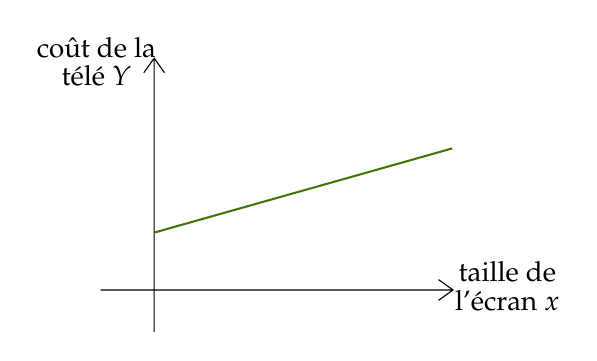
\begin{tikzpicture}[x=0.75pt,y=0.75pt,yscale=-1,xscale=1]
%uncomment if require: \path (0,300); %set diagram left start at 0, and has height of 300

%Shape: Axis 2D [id:dp3720388407437436] 
\draw  (50,144.67) -- (219.83,144.67)(75.83,33) -- (75.83,165) (212.83,139.67) -- (219.83,144.67) -- (212.83,149.67) (70.83,40) -- (75.83,33) -- (80.83,40)  ;
%Straight Lines [id:da45260329028360524] 
\draw [color={rgb, 255:red, 65; green, 117; blue, 5 }  ,draw opacity=1 ][line width=0.75]    (76.05,116.98) -- (219.41,76.48) ;

% Text Node
\draw (246,142.67) node   [align=left] {\shortstack{taille de\\ l'écran $x$}};
% Text Node
\draw (48,34.67) node   [align=left] {\shortstack{coût de la \\ télé $Y$}};


\end{tikzpicture}

\end{center}

L'intuition est que ton ami se base uniquement sur la taille de l'écran comme information pour deviner le coût. Une régression \textbf{linéaire} simple applique un facteur \textbf{multiplicatif}. Il ne peut pas se dire que plus grand l'écran est grand, plus le prix va augmenter---ceci serait plutôt une régression avec un paramètre \textbf{exponentiel}. 

On crée donc un facteur surnommé "paramètre". Dans le cas d'une régression linéaire simple, on a deux paramètres d'intérêts: un "niveau de base" pour le coût $\beta_{0}$ et un "multiplicateur" de la taille d'écran $\beta_{1}$:
\begin{center}
\tikzset{every picture/.style={line width=0.75pt}} %set default line width to 0.75pt        

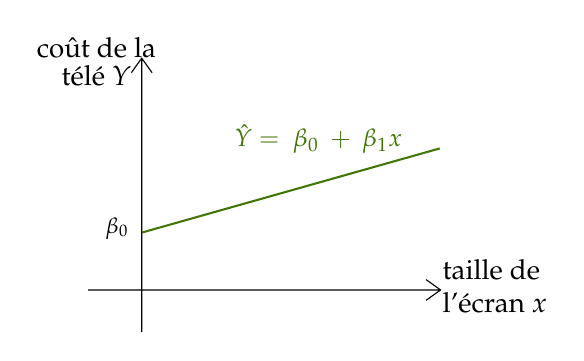
\begin{tikzpicture}[x=0.75pt,y=0.75pt,yscale=-1,xscale=1]
%uncomment if require: \path (0,300); %set diagram left start at 0, and has height of 300

%Shape: Axis 2D [id:dp3720388407437436] 
\draw  (50,144.67) -- (219.83,144.67)(75.83,33) -- (75.83,165) (212.83,139.67) -- (219.83,144.67) -- (212.83,149.67) (70.83,40) -- (75.83,33) -- (80.83,40)  ;
%Straight Lines [id:da45260329028360524] 
\draw [color={rgb, 255:red, 65; green, 117; blue, 5 }  ,draw opacity=1 ][line width=0.75]    (76.05,116.98) -- (219.41,76.48) ;

% Text Node
\draw (246,142.67) node   [align=left] {taille de\\ l'écran $x$};
% Text Node
\draw (54,34.67) node   [align=left] {\shortstack{coût de la \\ télé $Y$}};

% Text Node
\draw (64,115) node  [font=\footnotesize] [align=left] {$\beta _{0}$};
% Text Node
\draw (161,72) node  [font=\small,color={rgb, 255:red, 65; green, 117; blue, 5 }  ,opacity=1 ] [align=left] {$\hat{Y} =\ \beta _{0} \ +\ \beta _{1} x$};


\end{tikzpicture}

\end{center}

On suppose qu'une télé doit coûter au moins un certain prix. Ce "niveau de base" est l'intercepte sur le graphique ci-dessus surnommé l'ordonnée $\beta_{0}$. De ton gré, tu supposes au moins $\beta_{0} = 200\$$ pour cet exemple. 

Ensuite, le multiplicateur va multiplier la taille de l'écran pour obtenir un prix. Ce paramètre représente donc la pente $\beta_{1}$. De ton gré, tu suppose une pente de $\beta_{1} = 2\$$ pour cet exemple. 

Le coût (l'axe des $Y$) est la variable qui dépend de la taille---c'est la variable "dépendante" $Y$. La taille (l'axe des $x$) est la variable que l'on connaît indépendamment du coût---c'est la variable "indépendante" $x$. 

Finalement la droite elle-même est le coût que le modèle devine $\hat{Y}$. Le chapeau signifie que c'est une estimation, ou "prévision".

Par exemple, le modèle devine que le prix d'une télé de 50" est de 300\$; soit, $\hat{Y} = \beta_{0} + \beta_{1} x = 200 + (2) \cdot (50) = 300$. Selon le modèle, on estime que le coût de la télé est de 300\$.

Supposons que tu connais le \textit{vrai} coût $Y$, alors tu peux mesurer à quel point tu est dans le champ. Supposons que le vrai coût est de $Y = 400\$$. Alors, l'erreur dans ta prédiction est de $\varepsilon = 400 - 300 = 100\$$. 

Graphiquement:


\tikzset{every picture/.style={line width=0.75pt}} %set default line width to 0.75pt        

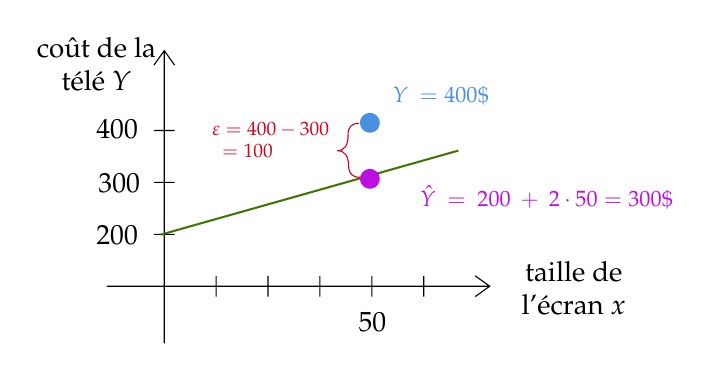
\begin{tikzpicture}[x=0.75pt,y=0.75pt,yscale=-1,xscale=1]
%uncomment if require: \path (0,300); %set diagram left start at 0, and has height of 300

%Shape: Axis 2D [id:dp0590336014536994] 
\draw  (50,141.82) -- (234.5,141.82)(77.7,28.33) -- (77.7,169.33) (227.5,136.82) -- (234.5,141.82) -- (227.5,146.82) (72.7,35.33) -- (77.7,28.33) -- (82.7,35.33) (102.7,136.82) -- (102.7,146.82)(127.7,136.82) -- (127.7,146.82)(152.7,136.82) -- (152.7,146.82)(177.7,136.82) -- (177.7,146.82)(202.7,136.82) -- (202.7,146.82)(72.7,116.82) -- (82.7,116.82)(72.7,91.82) -- (82.7,91.82)(72.7,66.82) -- (82.7,66.82) ;
\draw   ;
%Straight Lines [id:da6064475343931128] 
\draw [color={rgb, 255:red, 65; green, 117; blue, 5 }  ,draw opacity=1 ][line width=0.75]    (76.05,116.98) -- (219.41,76.48) ;
%Flowchart: Connector [id:dp8477117117153217] 
\draw  [draw opacity=0][fill={rgb, 255:red, 189; green, 16; blue, 224 }  ,fill opacity=1 ][line width=3]  (173.73,93.81) .. controls (171.68,92.14) and (171.38,89.12) .. (173.05,87.07) .. controls (174.72,85.02) and (177.74,84.71) .. (179.79,86.39) .. controls (181.84,88.06) and (182.15,91.08) .. (180.48,93.13) .. controls (178.8,95.18) and (175.79,95.49) .. (173.73,93.81) -- cycle ;
%Flowchart: Connector [id:dp4707804099581703] 
\draw  [draw opacity=0][fill={rgb, 255:red, 74; green, 144; blue, 226 }  ,fill opacity=1 ][line width=3]  (173.73,66.81) .. controls (171.68,65.14) and (171.38,62.12) .. (173.05,60.07) .. controls (174.72,58.02) and (177.74,57.71) .. (179.79,59.39) .. controls (181.84,61.06) and (182.15,64.08) .. (180.48,66.13) .. controls (178.8,68.18) and (175.79,68.49) .. (173.73,66.81) -- cycle ;
%Shape: Brace [id:dp37242003440355953] 
\draw  [color={rgb, 255:red, 208; green, 2; blue, 27 }  ,draw opacity=1 ] (171.5,63.33) .. controls (167.93,63.4) and (166.18,65.22) .. (166.25,68.79) -- (166.25,68.79) .. controls (166.35,73.89) and (164.61,76.47) .. (161.04,76.54) .. controls (164.61,76.47) and (166.45,78.99) .. (166.54,84.08)(166.5,81.79) -- (166.54,84.08) .. controls (166.61,87.65) and (168.43,89.4) .. (172,89.33) ;

% Text Node
\draw (275,142.67) node   [align=center] {taille de\\ l'écran $x$};
% Text Node
\draw (45,34.67) node   [align=center] {coût de la \\ télé $Y$};

% Text Node
\draw (262,99) node  [font=\footnotesize,color={rgb, 255:red, 189; green, 16; blue, 224 }  ,opacity=1 ] [align=left] {$\displaystyle \hat{Y} \ =\ 200\ +\ 2\cdot 50=300\$$};
% Text Node
\draw (55,117.33) node   [align=left] {$\displaystyle 200$};
% Text Node
\draw (56,92.33) node   [align=left] {$\displaystyle 300$};
% Text Node
\draw (55,66.33) node   [align=left] {$\displaystyle 400$};
% Text Node
\draw (211,50) node  [font=\footnotesize,color={rgb, 255:red, 74; green, 144; blue, 226 }  ,opacity=1 ] [align=left] {$\displaystyle Y\ =400\$$};
% Text Node
\draw (129,72.33) node  [font=\scriptsize,color={rgb, 255:red, 208; green, 2; blue, 27 }  ,opacity=1 ] [align=left] {$\displaystyle  \begin{array}{{>{\displaystyle}l}}
\varepsilon =400-300\\
\ \ =100
\end{array}$};
% Text Node
\draw (178,159.33) node   [align=left] {$\displaystyle 50$};


\end{tikzpicture}

On voit donc que $Y = \beta_{0} + \beta_{1} x + \varepsilon$ est un "modèle" théorique pour obtenir une variable dépendante $Y$ en fonction de: 
\begin{itemize}
	\item	Une variable indépendante $x$ multipliée par un facteur $\beta_{1}$.
	\item	Un niveau de base l'intercepte $\beta_{0}$.
	\item	Une erreur aléatoire $\varepsilon$ inconnue.
\end{itemize}

\section{Autres}
\textbf{Matrice de confusion : }
\begin{center}


\tikzset{every picture/.style={line width=0.75pt}} %set default line width to 0.75pt        

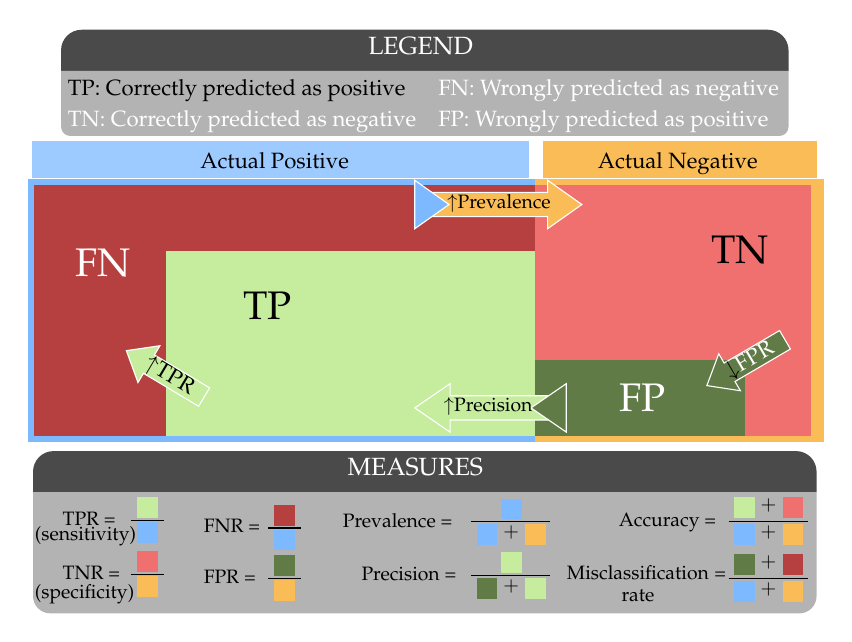
\begin{tikzpicture}[x=0.75pt,y=0.75pt,yscale=-1,xscale=1]
%uncomment if require: \path (0,366); %set diagram left start at 0, and has height of 366

%Rounded Same Side Corner Rect [id:dp5863189014777732] 
\draw  [draw opacity=0][fill={rgb, 255:red, 74; green, 74; blue, 74 }  ,fill opacity=1 ][line width=1.5]  (186.37,215.03) .. controls (186.37,209.57) and (190.8,205.14) .. (196.27,205.14) -- (553.98,205.14) .. controls (559.45,205.14) and (563.87,209.57) .. (563.87,215.03) -- (563.87,224.92) .. controls (563.87,224.92) and (563.87,224.92) .. (563.87,224.92) -- (186.37,224.92) .. controls (186.37,224.92) and (186.37,224.92) .. (186.37,224.92) -- cycle ;
%Rounded Same Side Corner Rect [id:dp10542736831068278] 
\draw  [draw opacity=0][fill={rgb, 255:red, 179; green, 179; blue, 179 }  ,fill opacity=1 ] (563.87,275.01) .. controls (563.87,279.61) and (560.15,283.33) .. (555.56,283.33) -- (194.69,283.33) .. controls (190.1,283.33) and (186.37,279.61) .. (186.37,275.01) -- (186.37,224.92) .. controls (186.37,224.92) and (186.37,224.92) .. (186.37,224.92) -- (563.87,224.92) .. controls (563.87,224.92) and (563.87,224.92) .. (563.87,224.92) -- cycle ;
%Flowchart: Process [id:dp2781782458228159] 
\draw  [draw opacity=0][fill={rgb, 255:red, 198; green, 237; blue, 158 }  ,fill opacity=1 ] (236.54,237.33) -- (246.54,237.33) -- (246.54,227.33) -- (236.54,227.33) -- cycle ;
%Flowchart: Process [id:dp6595006333689621] 
\draw  [draw opacity=0][fill={rgb, 255:red, 125; green, 185; blue, 255 }  ,fill opacity=1 ] (236.54,249.33) -- (246.54,249.33) -- (246.54,239.33) -- (236.54,239.33) -- cycle ;
%Straight Lines [id:da005645386209309766] 
\draw    (233.54,238.5) -- (249.54,238.5) ;

%Flowchart: Process [id:dp7524991543129134] 
\draw  [draw opacity=0][fill={rgb, 255:red, 125; green, 185; blue, 255 }  ,fill opacity=1 ] (302.54,253) -- (312.54,253) -- (312.54,243) -- (302.54,243) -- cycle ;
%Straight Lines [id:da5176971400521515] 
\draw    (299.54,242.17) -- (315.54,242.17) ;
%Flowchart: Process [id:dp9574550023533219] 
\draw  [draw opacity=0][fill={rgb, 255:red, 182; green, 64; blue, 64 }  ,fill opacity=1 ] (302.54,241) -- (312.54,241) -- (312.54,231) -- (302.54,231) -- cycle ;

%Flowchart: Process [id:dp6446573608226225] 
\draw  [draw opacity=0][fill={rgb, 255:red, 240; green, 111; blue, 111 }  ,fill opacity=1 ] (236.54,263.5) -- (246.54,263.5) -- (246.54,253.5) -- (236.54,253.5) -- cycle ;
%Flowchart: Process [id:dp6670926329350344] 
\draw  [draw opacity=0][fill={rgb, 255:red, 249; green, 188; blue, 87 }  ,fill opacity=1 ] (236.54,275.5) -- (246.54,275.5) -- (246.54,265.5) -- (236.54,265.5) -- cycle ;
%Straight Lines [id:da5832941059999399] 
\draw    (233.54,264.67) -- (249.54,264.67) ;

%Flowchart: Process [id:dp3885928458657999] 
\draw  [draw opacity=0][fill={rgb, 255:red, 249; green, 188; blue, 87 }  ,fill opacity=1 ] (302.54,277.33) -- (312.54,277.33) -- (312.54,267.33) -- (302.54,267.33) -- cycle ;
%Straight Lines [id:da3401710446338324] 
\draw    (299.54,266.5) -- (315.54,266.5) ;
%Flowchart: Process [id:dp6813365938208455] 
\draw  [draw opacity=0][fill={rgb, 255:red, 97; green, 123; blue, 71 }  ,fill opacity=1 ] (302.54,265.33) -- (312.54,265.33) -- (312.54,255.33) -- (302.54,255.33) -- cycle ;

%Flowchart: Process [id:dp26333217881412674] 
\draw  [draw opacity=0][fill={rgb, 255:red, 198; green, 237; blue, 158 }  ,fill opacity=1 ] (412.04,263.83) -- (422.04,263.83) -- (422.04,253.83) -- (412.04,253.83) -- cycle ;
%Flowchart: Process [id:dp33935301348671065] 
\draw  [draw opacity=0][fill={rgb, 255:red, 97; green, 123; blue, 71 }  ,fill opacity=1 ] (400.04,276.33) -- (410.04,276.33) -- (410.04,266.33) -- (400.04,266.33) -- cycle ;
%Straight Lines [id:da4578404875999813] 
\draw    (397.54,265) -- (435.54,265) ;
%Flowchart: Process [id:dp07704188689930547] 
\draw  [draw opacity=0][fill={rgb, 255:red, 198; green, 237; blue, 158 }  ,fill opacity=1 ] (423.54,276.33) -- (433.54,276.33) -- (433.54,266.33) -- (423.54,266.33) -- cycle ;

%Flowchart: Process [id:dp511192763925254] 
\draw  [draw opacity=0][fill={rgb, 255:red, 125; green, 185; blue, 255 }  ,fill opacity=1 ] (412.04,238) -- (422.04,238) -- (422.04,228) -- (412.04,228) -- cycle ;
%Flowchart: Process [id:dp8487027222224734] 
\draw  [draw opacity=0][fill={rgb, 255:red, 125; green, 185; blue, 255 }  ,fill opacity=1 ] (400.04,250.5) -- (410.04,250.5) -- (410.04,240.5) -- (400.04,240.5) -- cycle ;
%Straight Lines [id:da11748805900160852] 
\draw    (397.54,239.17) -- (435.54,239.17) ;
%Flowchart: Process [id:dp6757535243694623] 
\draw  [draw opacity=0][fill={rgb, 255:red, 249; green, 188; blue, 87 }  ,fill opacity=1 ] (423.54,250.5) -- (433.54,250.5) -- (433.54,240.5) -- (423.54,240.5) -- cycle ;

%Flowchart: Process [id:dp23257062904433523] 
\draw  [draw opacity=0][fill={rgb, 255:red, 125; green, 185; blue, 255 }  ,fill opacity=1 ] (524.04,250.5) -- (534.04,250.5) -- (534.04,240.5) -- (524.04,240.5) -- cycle ;
%Straight Lines [id:da16879793480007654] 
\draw    (521.54,239.17) -- (559.54,239.17) ;
%Flowchart: Process [id:dp629293047660624] 
\draw  [draw opacity=0][fill={rgb, 255:red, 249; green, 188; blue, 87 }  ,fill opacity=1 ] (547.54,250.5) -- (557.54,250.5) -- (557.54,240.5) -- (547.54,240.5) -- cycle ;
%Flowchart: Process [id:dp25903639593069716] 
\draw  [draw opacity=0][fill={rgb, 255:red, 198; green, 237; blue, 158 }  ,fill opacity=1 ] (524.04,237.5) -- (534.04,237.5) -- (534.04,227.5) -- (524.04,227.5) -- cycle ;
%Flowchart: Process [id:dp2784202862814029] 
\draw  [draw opacity=0][fill={rgb, 255:red, 240; green, 111; blue, 111 }  ,fill opacity=1 ] (547.54,237.5) -- (557.54,237.5) -- (557.54,227.5) -- (547.54,227.5) -- cycle ;

%Flowchart: Process [id:dp5706215732887201] 
\draw  [draw opacity=0][fill={rgb, 255:red, 125; green, 185; blue, 255 }  ,fill opacity=1 ] (524.04,277.83) -- (534.04,277.83) -- (534.04,267.83) -- (524.04,267.83) -- cycle ;
%Straight Lines [id:da24052635124853383] 
\draw    (521.54,266.5) -- (559.54,266.5) ;
%Flowchart: Process [id:dp8806206355646873] 
\draw  [draw opacity=0][fill={rgb, 255:red, 249; green, 188; blue, 87 }  ,fill opacity=1 ] (547.54,277.83) -- (557.54,277.83) -- (557.54,267.83) -- (547.54,267.83) -- cycle ;
%Flowchart: Process [id:dp025661689438194246] 
\draw  [draw opacity=0][fill={rgb, 255:red, 97; green, 123; blue, 71 }  ,fill opacity=1 ] (524.04,264.83) -- (534.04,264.83) -- (534.04,254.83) -- (524.04,254.83) -- cycle ;
%Flowchart: Process [id:dp07416724651822326] 
\draw  [draw opacity=0][fill={rgb, 255:red, 182; green, 64; blue, 64 }  ,fill opacity=1 ] (547.54,264.83) -- (557.54,264.83) -- (557.54,254.83) -- (547.54,254.83) -- cycle ;


%Shape: Rectangle [id:dp9078887636984747] 
\draw  [color={rgb, 255:red, 125; green, 185; blue, 255 }  ,draw opacity=1 ][fill={rgb, 255:red, 125; green, 185; blue, 255 }  ,fill opacity=1 ][line width=4.5]  (186.79,76.98) -- (428.29,76.98) -- (428.29,198) -- (186.79,198) -- cycle ;
%Shape: Rectangle [id:dp6719473196737591] 
\draw  [color={rgb, 255:red, 249; green, 188; blue, 87 }  ,draw opacity=1 ][fill={rgb, 255:red, 249; green, 188; blue, 87 }  ,fill opacity=1 ][line width=4.5]  (431.29,76.98) -- (564.29,76.98) -- (564.29,198) -- (431.29,198) -- cycle ;
%Shape: Rectangle [id:dp8554811027992568] 
\draw  [draw opacity=0][fill={rgb, 255:red, 240; green, 111; blue, 111 }  ,fill opacity=1 ][line width=0.75]  (427.96,76.98) -- (560.96,76.98) -- (560.96,198) -- (427.96,198) -- cycle ;
%Shape: Rectangle [id:dp4666790964474916] 
\draw  [draw opacity=0][fill={rgb, 255:red, 182; green, 64; blue, 64 }  ,fill opacity=1 ] (186.79,76.98) -- (428.29,76.98) -- (428.29,198) -- (186.79,198) -- cycle ;
%Shape: Rectangle [id:dp4684932062372884] 
\draw  [draw opacity=0][fill={rgb, 255:red, 125; green, 185; blue, 255 }  ,fill opacity=0.75 ] (185.96,55.67) -- (425.29,55.67) -- (425.29,73.33) -- (185.96,73.33) -- cycle ;
%Shape: Rectangle [id:dp7538608016518991] 
\draw  [draw opacity=0][fill={rgb, 255:red, 249; green, 188; blue, 87 }  ,fill opacity=1 ] (432.29,55.67) -- (563.96,55.67) -- (563.96,73.33) -- (432.29,73.33) -- cycle ;
%Shape: Rectangle [id:dp575388567694743] 
\draw  [draw opacity=0][fill={rgb, 255:red, 198; green, 237; blue, 158 }  ,fill opacity=1 ] (250.29,108.8) -- (428.29,108.8) -- (428.29,198) -- (250.29,198) -- cycle ;
%Shape: Rectangle [id:dp694025502587706] 
\draw  [draw opacity=0][fill={rgb, 255:red, 97; green, 123; blue, 71 }  ,fill opacity=1 ] (428.29,161.33) -- (529.29,161.33) -- (529.29,198) -- (428.29,198) -- cycle ;
%Left Arrow [id:dp159442790435544] 
\draw  [color={rgb, 255:red, 255; green, 255; blue, 255 }  ,draw opacity=1 ][fill={rgb, 255:red, 97; green, 123; blue, 71 }  ,fill opacity=1 ] (511.02,173.58) -- (516.74,158.26) -- (519.35,162.71) -- (546.06,147.06) -- (551.28,155.96) -- (524.57,171.61) -- (527.18,176.07) -- cycle ;

%Left Arrow [id:dp2567253964557259] 
\draw  [color={rgb, 255:red, 255; green, 255; blue, 255 }  ,draw opacity=1 ][fill={rgb, 255:red, 198; green, 237; blue, 158 }  ,fill opacity=1 ] (231.33,156.74) -- (247.51,154.38) -- (244.87,158.81) -- (271.45,174.68) -- (266.16,183.54) -- (239.58,167.67) -- (236.93,172.1) -- cycle ;

%Left Arrow [id:dp4712888920317464] 
\draw  [color={rgb, 255:red, 255; green, 255; blue, 255 }  ,draw opacity=1 ][fill={rgb, 255:red, 198; green, 237; blue, 158 }  ,fill opacity=1 ] (370.29,184.33) -- (387.29,172.66) -- (387.29,178.5) -- (440.29,178.5) -- (440.29,190.17) -- (387.29,190.17) -- (387.29,196) -- cycle ;
%Left Arrow [id:dp3521145387427629] 
\draw  [color={rgb, 255:red, 255; green, 255; blue, 255 }  ,draw opacity=1 ][fill={rgb, 255:red, 97; green, 123; blue, 71 }  ,fill opacity=1 ] (426.29,184.33) -- (443.29,172.66) -- (443.29,178.5) -- (443.29,178.5) -- (443.29,190.17) -- (443.29,190.17) -- (443.29,196) -- cycle ;

%Left Arrow [id:dp8166384807624658] 
\draw  [color={rgb, 255:red, 255; green, 255; blue, 255 }  ,draw opacity=1 ][fill={rgb, 255:red, 249; green, 188; blue, 87 }  ,fill opacity=1 ] (450.8,86.33) -- (434.29,74.66) -- (434.29,80.5) -- (370.29,80.5) -- (370.29,92.17) -- (434.29,92.17) -- (434.29,98) -- cycle ;
%Left Arrow [id:dp8194414952038565] 
\draw  [color={rgb, 255:red, 255; green, 255; blue, 255 }  ,draw opacity=1 ][fill={rgb, 255:red, 125; green, 185; blue, 255 }  ,fill opacity=1 ] (386.8,86.33) -- (370.29,74.66) -- (370.29,80.5) -- (370.29,80.5) -- (370.29,92.17) -- (370.29,92.17) -- (370.29,98) -- cycle ;


%Rounded Same Side Corner Rect [id:dp01839882980964913] 
\draw  [draw opacity=0][fill={rgb, 255:red, 74; green, 74; blue, 74 }  ,fill opacity=1 ][line width=1.5]  (199.87,12.03) .. controls (199.87,6.57) and (204.3,2.14) .. (209.77,2.14) -- (540.48,2.14) .. controls (545.95,2.14) and (550.37,6.57) .. (550.37,12.03) -- (550.37,21.92) .. controls (550.37,21.92) and (550.37,21.92) .. (550.37,21.92) -- (199.87,21.92) .. controls (199.87,21.92) and (199.87,21.92) .. (199.87,21.92) -- cycle ;
%Rounded Same Side Corner Rect [id:dp42232070994654003] 
\draw  [draw opacity=0][fill={rgb, 255:red, 179; green, 179; blue, 179 }  ,fill opacity=1 ] (550.37,48.86) .. controls (550.37,51.33) and (548.37,53.33) .. (545.9,53.33) -- (204.35,53.33) .. controls (201.88,53.33) and (199.87,51.33) .. (199.87,48.86) -- (199.87,21.92) .. controls (199.87,21.92) and (199.87,21.92) .. (199.87,21.92) -- (550.37,21.92) .. controls (550.37,21.92) and (550.37,21.92) .. (550.37,21.92) -- cycle ;


% Text Node
\draw (267.37,236.67) node [anchor=north west][inner sep=0.75pt]  [font=\scriptsize] [align=left] {FNR = };
% Text Node
\draw (267.37,261) node [anchor=north west][inner sep=0.75pt]  [font=\scriptsize] [align=left] {FPR = };
% Text Node
\draw (343.37,259.5) node [anchor=north west][inner sep=0.75pt]  [font=\scriptsize] [align=left] {Precision = };
% Text Node
\draw (411.54,265.83) node [anchor=north west][inner sep=0.75pt]  [font=\scriptsize] [align=left] {$\displaystyle +$};
% Text Node
\draw (535.54,267.33) node [anchor=north west][inner sep=0.75pt]  [font=\scriptsize] [align=left] {$\displaystyle +$};
% Text Node
\draw (440.37,259) node [anchor=north west][inner sep=0.75pt]  [font=\scriptsize] [align=left] {\begin{minipage}[lt]{54.30085600000001pt}\setlength\topsep{0pt}
\begin{center}
Misclassification\\rate 
\end{center}

\end{minipage}};
% Text Node
\draw (535.54,254.33) node [anchor=north west][inner sep=0.75pt]  [font=\scriptsize] [align=left] {$\displaystyle +$};
% Text Node
\draw (513.37,262) node [anchor=north west][inner sep=0.75pt]  [font=\scriptsize] [align=left] {= };
% Text Node
\draw (535.54,240) node [anchor=north west][inner sep=0.75pt]  [font=\scriptsize] [align=left] {$\displaystyle +$};
% Text Node
\draw (467.37,233.67) node [anchor=north west][inner sep=0.75pt]  [font=\scriptsize] [align=left] {Accuracy = };
% Text Node
\draw (535.54,227) node [anchor=north west][inner sep=0.75pt]  [font=\scriptsize] [align=left] {$\displaystyle +$};
% Text Node
\draw (334.37,233.67) node [anchor=north west][inner sep=0.75pt]  [font=\scriptsize] [align=left] {Prevalence = };
% Text Node
\draw (411.54,240) node [anchor=north west][inner sep=0.75pt]  [font=\scriptsize] [align=left] {$\displaystyle +$};
% Text Node
\draw (243.09,156.56) node [anchor=north west][inner sep=0.75pt]  [font=\scriptsize,rotate=-30.84] [align=left] {{\footnotesize $\displaystyle \uparrow $TPR}};
% Text Node
\draw (516.52,163.19) node [anchor=north west][inner sep=0.75pt]  [font=\scriptsize,rotate=-329.62] [align=left] {{\footnotesize $\displaystyle \downarrow $\textcolor[rgb]{1,1,1}{FPR}}};
% Text Node
\draw (382.95,178.25) node [anchor=north west][inner sep=0.75pt]  [font=\scriptsize] [align=left] {{\scriptsize $\displaystyle \uparrow $Precision}};
% Text Node
\draw (384.63,80.25) node [anchor=north west][inner sep=0.75pt]  [font=\scriptsize] [align=left] {{\scriptsize $\displaystyle \uparrow $Prevalence}};
% Text Node
\draw (199.37,233) node [anchor=north west][inner sep=0.75pt]  [font=\scriptsize] [align=left] {TPR = };
% Text Node
\draw (186,240) node [anchor=north west][inner sep=0.75pt]  [font=\scriptsize] [align=left] {{\scriptsize (sensitivity)}};
% Text Node
\draw (199.37,259.17) node [anchor=north west][inner sep=0.75pt]  [font=\scriptsize] [align=left] {TNR = };
% Text Node
\draw (186,268.17) node [anchor=north west][inner sep=0.75pt]  [font=\scriptsize] [align=left] {{\scriptsize (specificity)}};
% Text Node
\draw (264.04,60.17) node [anchor=north west][inner sep=0.75pt]  [font=\footnotesize,color={rgb, 255:red, 0; green, 0; blue, 0 }  ,opacity=1 ] [align=left] {\begin{minipage}[lt]{56.241644pt}\setlength\topsep{0pt}
\begin{center}
Actual Positive
\end{center}

\end{minipage}};
% Text Node
\draw (455.79,60.17) node [anchor=north west][inner sep=0.75pt]  [font=\footnotesize,color={rgb, 255:red, 0; green, 0; blue, 0 }  ,opacity=1 ] [align=left] {\begin{minipage}[lt]{59.875428pt}\setlength\topsep{0pt}
\begin{center}
Actual Negative
\end{center}

\end{minipage}};
% Text Node
\draw (464.29,171.17) node [anchor=north west][inner sep=0.75pt]  [font=\Large,color={rgb, 255:red, 255; green, 255; blue, 255 }  ,opacity=1 ] [align=left] {\begin{minipage}[lt]{21.490856pt}\setlength\topsep{0pt}
\begin{center}\textcolor{white}{
FP}
\end{center}

\end{minipage}};
% Text Node
\draw (204.04,106.17) node [anchor=north west][inner sep=0.75pt]  [font=\Large,color={rgb, 255:red, 255; green, 255; blue, 255 }  ,opacity=1 ] [align=left] {\begin{minipage}[lt]{22.305428000000003pt}\setlength\topsep{0pt}
\begin{center}\textcolor{white}{
FN}
\end{center}

\end{minipage}};
% Text Node
\draw (510.96,99.99) node [anchor=north west][inner sep=0.75pt]  [font=\Large,color={rgb, 255:red, 0; green, 0; blue, 0 }  ,opacity=1 ] [align=left] {\begin{minipage}[lt]{22.305428000000003pt}\setlength\topsep{0pt}
\begin{center}
TN
\end{center}

\end{minipage}};
% Text Node
\draw (283.79,126.9) node [anchor=north west][inner sep=0.75pt]  [font=\Large,color={rgb, 255:red, 0; green, 0; blue, 0 }  ,opacity=1 ] [align=left] {\begin{minipage}[lt]{21.490856pt}\setlength\topsep{0pt}
\begin{center}
TP
\end{center}

\end{minipage}};
% Text Node
\draw (336.62,207.19) node [anchor=north west][inner sep=0.75pt]  [font=\small,color={rgb, 255:red, 255; green, 255; blue, 255 }  ,opacity=1 ] [align=left] {MEASURES};
% Text Node
\draw (346.62,4.53) node [anchor=north west][inner sep=0.75pt]  [font=\small,color={rgb, 255:red, 255; green, 255; blue, 255 }  ,opacity=1 ] [align=left] {LEGEND};
% Text Node
\draw (201.87,24.92) node [anchor=north west][inner sep=0.75pt]  [font=\small,color={rgb, 255:red, 255; green, 255; blue, 255 }  ,opacity=1 ] [align=left] {{\footnotesize \textcolor[rgb]{0,0,0}{TP: Correctly predicted as positive}}\\{\footnotesize TN: Correctly predicted as negative}};
% Text Node
\draw (380.37,24.92) node [anchor=north west][inner sep=0.75pt]  [font=\small,color={rgb, 255:red, 255; green, 255; blue, 255 }  ,opacity=1 ] [align=left] {{\footnotesize FN: Wrongly predicted as negative}\\{\footnotesize FP: Wrongly predicted as positive}};


\end{tikzpicture}
\end{center}


\section{Erreur}

\begin{description}
	\item[Écart-type]	Mesure la variation \underline{entre les observations} d'\textbf{un} ensemble de données.
		\begin{itemize}[leftmargin = *]
		\item	\og \textit{standard deviation} \fg{}.
		\end{itemize}
		\begin{center}

\tikzset{every picture/.style={line width=0.75pt}} %set default line width to 0.75pt        

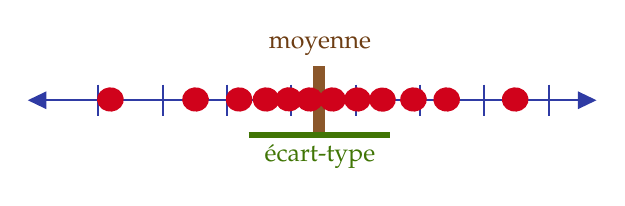
\begin{tikzpicture}[x=0.75pt,y=0.75pt,yscale=-1,xscale=1]
%uncomment if require: \path (0,174); %set diagram left start at 0, and has height of 174

%Straight Lines [id:da5554502737558269] 
\draw [color={rgb, 255:red, 47; green, 59; blue, 164 }  ,draw opacity=1 ][line width=0.75]    (279.83,38) -- (547.83,38) (310.83,30.5) -- (310.83,45.5)(341.83,30.5) -- (341.83,45.5)(372.83,30.5) -- (372.83,45.5)(403.83,30.5) -- (403.83,45.5)(434.83,30.5) -- (434.83,45.5)(465.83,30.5) -- (465.83,45.5)(496.83,30.5) -- (496.83,45.5)(527.83,30.5) -- (527.83,45.5) ;
\draw [shift={(550.83,38)}, rotate = 180] [fill={rgb, 255:red, 47; green, 59; blue, 164 }  ,fill opacity=1 ][line width=0.08]  [draw opacity=0] (8.93,-4.29) -- (0,0) -- (8.93,4.29) -- cycle    ;
\draw [shift={(276.83,38)}, rotate = 0] [fill={rgb, 255:red, 47; green, 59; blue, 164 }  ,fill opacity=1 ][line width=0.08]  [draw opacity=0] (8.93,-4.29) -- (0,0) -- (8.93,4.29) -- cycle    ;
%Straight Lines [id:da6666232383065853] 
\draw [color={rgb, 255:red, 139; green, 87; blue, 42 }  ,draw opacity=1 ][line width=2.25]    (415.67,54.92) -- (415.67,21.42)(418.67,54.92) -- (418.67,21.42) ;
%Flowchart: Connector [id:dp30389051575543746] 
\draw  [draw opacity=0][fill={rgb, 255:red, 208; green, 2; blue, 27 }  ,fill opacity=1 ] (320.71,33.09) .. controls (317.96,31.04) and (313.9,31.42) .. (311.65,33.93) .. controls (309.4,36.44) and (309.81,40.13) .. (312.57,42.17) .. controls (315.33,44.21) and (319.39,43.84) .. (321.63,41.33) .. controls (323.88,38.82) and (323.47,35.13) .. (320.71,33.09) -- cycle ;
%Flowchart: Connector [id:dp8054636909486927] 
\draw  [draw opacity=0][fill={rgb, 255:red, 208; green, 2; blue, 27 }  ,fill opacity=1 ] (382.71,33.09) .. controls (379.96,31.04) and (375.9,31.42) .. (373.65,33.93) .. controls (371.4,36.44) and (371.81,40.13) .. (374.57,42.17) .. controls (377.33,44.21) and (381.39,43.84) .. (383.63,41.33) .. controls (385.88,38.82) and (385.47,35.13) .. (382.71,33.09) -- cycle ;
%Flowchart: Connector [id:dp4481822183684774] 
\draw  [draw opacity=0][fill={rgb, 255:red, 208; green, 2; blue, 27 }  ,fill opacity=1 ] (361.71,33.09) .. controls (358.96,31.04) and (354.9,31.42) .. (352.65,33.93) .. controls (350.4,36.44) and (350.81,40.13) .. (353.57,42.17) .. controls (356.33,44.21) and (360.39,43.84) .. (362.63,41.33) .. controls (364.88,38.82) and (364.47,35.13) .. (361.71,33.09) -- cycle ;
%Flowchart: Connector [id:dp9320426369464008] 
\draw  [draw opacity=0][fill={rgb, 255:red, 208; green, 2; blue, 27 }  ,fill opacity=1 ] (416.71,33.09) .. controls (413.96,31.04) and (409.9,31.42) .. (407.65,33.93) .. controls (405.4,36.44) and (405.81,40.13) .. (408.57,42.17) .. controls (411.33,44.21) and (415.39,43.84) .. (417.63,41.33) .. controls (419.88,38.82) and (419.47,35.13) .. (416.71,33.09) -- cycle ;
%Flowchart: Connector [id:dp5645916521008547] 
\draw  [draw opacity=0][fill={rgb, 255:red, 208; green, 2; blue, 27 }  ,fill opacity=1 ] (395.71,33.09) .. controls (392.96,31.04) and (388.9,31.42) .. (386.65,33.93) .. controls (384.4,36.44) and (384.81,40.13) .. (387.57,42.17) .. controls (390.33,44.21) and (394.39,43.84) .. (396.63,41.33) .. controls (398.88,38.82) and (398.47,35.13) .. (395.71,33.09) -- cycle ;
%Flowchart: Connector [id:dp9615392127090878] 
\draw  [draw opacity=0][fill={rgb, 255:red, 208; green, 2; blue, 27 }  ,fill opacity=1 ] (439.71,33.09) .. controls (436.96,31.04) and (432.9,31.42) .. (430.65,33.93) .. controls (428.4,36.44) and (428.81,40.13) .. (431.57,42.17) .. controls (434.33,44.21) and (438.39,43.84) .. (440.63,41.33) .. controls (442.88,38.82) and (442.47,35.13) .. (439.71,33.09) -- cycle ;
%Flowchart: Connector [id:dp18343654664200626] 
\draw  [draw opacity=0][fill={rgb, 255:red, 208; green, 2; blue, 27 }  ,fill opacity=1 ] (427.71,33.09) .. controls (424.96,31.04) and (420.9,31.42) .. (418.65,33.93) .. controls (416.4,36.44) and (416.81,40.13) .. (419.57,42.17) .. controls (422.33,44.21) and (426.39,43.84) .. (428.63,41.33) .. controls (430.88,38.82) and (430.47,35.13) .. (427.71,33.09) -- cycle ;
%Flowchart: Connector [id:dp49357374316679636] 
\draw  [draw opacity=0][fill={rgb, 255:red, 208; green, 2; blue, 27 }  ,fill opacity=1 ] (466.71,33.09) .. controls (463.96,31.04) and (459.9,31.42) .. (457.65,33.93) .. controls (455.4,36.44) and (455.81,40.13) .. (458.57,42.17) .. controls (461.33,44.21) and (465.39,43.84) .. (467.63,41.33) .. controls (469.88,38.82) and (469.47,35.13) .. (466.71,33.09) -- cycle ;
%Flowchart: Connector [id:dp5732145021055151] 
\draw  [draw opacity=0][fill={rgb, 255:red, 208; green, 2; blue, 27 }  ,fill opacity=1 ] (451.78,33.16) .. controls (449.02,31.12) and (444.96,31.49) .. (442.71,34) .. controls (440.46,36.51) and (440.88,40.2) .. (443.63,42.24) .. controls (446.39,44.28) and (450.45,43.91) .. (452.7,41.4) .. controls (454.94,38.89) and (454.53,35.2) .. (451.78,33.16) -- cycle ;
%Flowchart: Connector [id:dp9989913792112952] 
\draw  [draw opacity=0][fill={rgb, 255:red, 208; green, 2; blue, 27 }  ,fill opacity=1 ] (515.71,33.09) .. controls (512.96,31.04) and (508.9,31.42) .. (506.65,33.93) .. controls (504.4,36.44) and (504.81,40.13) .. (507.57,42.17) .. controls (510.33,44.21) and (514.39,43.84) .. (516.63,41.33) .. controls (518.88,38.82) and (518.47,35.13) .. (515.71,33.09) -- cycle ;
%Flowchart: Connector [id:dp2709053942707078] 
\draw  [draw opacity=0][fill={rgb, 255:red, 208; green, 2; blue, 27 }  ,fill opacity=1 ] (482.71,33.09) .. controls (479.96,31.04) and (475.9,31.42) .. (473.65,33.93) .. controls (471.4,36.44) and (471.81,40.13) .. (474.57,42.17) .. controls (477.33,44.21) and (481.39,43.84) .. (483.63,41.33) .. controls (485.88,38.82) and (485.47,35.13) .. (482.71,33.09) -- cycle ;
%Flowchart: Connector [id:dp7446426173106822] 
\draw  [draw opacity=0][fill={rgb, 255:red, 208; green, 2; blue, 27 }  ,fill opacity=1 ] (406.65,33.02) .. controls (403.89,30.97) and (399.84,31.35) .. (397.59,33.86) .. controls (395.34,36.36) and (395.75,40.05) .. (398.51,42.1) .. controls (401.27,44.14) and (405.32,43.77) .. (407.57,41.26) .. controls (409.82,38.75) and (409.41,35.06) .. (406.65,33.02) -- cycle ;
%Straight Lines [id:da9789557877821047] 
\draw [color={rgb, 255:red, 65; green, 117; blue, 5 }  ,draw opacity=1 ][line width=2.25]    (383.17,54.92) -- (451.17,54.92) ;

% Text Node
\draw (417.58,12) node  [color={rgb, 255:red, 109; green, 61; blue, 19 }  ,opacity=1 ] [align=left] {{\small moyenne}};
% Text Node
\draw (417.58,65) node  [font=\small,color={rgb, 255:red, 109; green, 61; blue, 19 }  ,opacity=1 ] [align=left] {{\small \textcolor[rgb]{0.25,0.46,0.02}{écart-type}}};


\end{tikzpicture}
		\end{center}
	\item[Erreur type]	Mesure la variation \underline{entre les moyennes} de \textbf{plusieurs} ensembles de données.
		\begin{itemize}[leftmargin = *]
		\item	\og \textit{standard error} \fg{}.
		\end{itemize}
		\begin{center}
		

\tikzset{every picture/.style={line width=0.75pt}} %set default line width to 0.75pt        

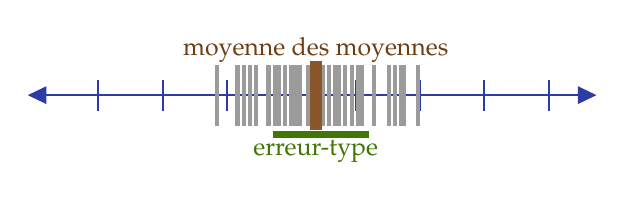
\begin{tikzpicture}[x=0.75pt,y=0.75pt,yscale=-1,xscale=1]
%uncomment if require: \path (0,174); %set diagram left start at 0, and has height of 174

%Straight Lines [id:da8220125436751056] 
\draw [color={rgb, 255:red, 47; green, 59; blue, 164 }  ,draw opacity=1 ][line width=0.75]    (281.83,118) -- (549.83,118) (312.83,110.5) -- (312.83,125.5)(343.83,110.5) -- (343.83,125.5)(374.83,110.5) -- (374.83,125.5)(405.83,110.5) -- (405.83,125.5)(436.83,110.5) -- (436.83,125.5)(467.83,110.5) -- (467.83,125.5)(498.83,110.5) -- (498.83,125.5)(529.83,110.5) -- (529.83,125.5) ;
\draw [shift={(552.83,118)}, rotate = 180] [fill={rgb, 255:red, 47; green, 59; blue, 164 }  ,fill opacity=1 ][line width=0.08]  [draw opacity=0] (8.93,-4.29) -- (0,0) -- (8.93,4.29) -- cycle    ;
\draw [shift={(278.83,118)}, rotate = 0] [fill={rgb, 255:red, 47; green, 59; blue, 164 }  ,fill opacity=1 ][line width=0.08]  [draw opacity=0] (8.93,-4.29) -- (0,0) -- (8.93,4.29) -- cycle    ;
%Straight Lines [id:da052261111869088106] 
\draw [color={rgb, 255:red, 155; green, 155; blue, 155 }  ,draw opacity=1 ][line width=1.5]    (415.83,132.67) -- (415.83,103.33) ;
%Straight Lines [id:da25533101510311673] 
\draw [color={rgb, 255:red, 155; green, 155; blue, 155 }  ,draw opacity=1 ][line width=1.5]    (420.83,132.67) -- (420.83,103.33) ;
%Straight Lines [id:da6426635244738363] 
\draw [color={rgb, 255:red, 155; green, 155; blue, 155 }  ,draw opacity=1 ][line width=1.5]    (426.83,132.67) -- (426.83,103.33) ;
%Straight Lines [id:da6924171841728055] 
\draw [color={rgb, 255:red, 155; green, 155; blue, 155 }  ,draw opacity=1 ][line width=1.5]    (423.83,132.67) -- (423.83,103.33) ;
%Straight Lines [id:da19673873838231448] 
\draw [color={rgb, 255:red, 155; green, 155; blue, 155 }  ,draw opacity=1 ][line width=1.5]    (428.83,132.67) -- (428.83,103.33) ;
%Straight Lines [id:da9733057591182157] 
\draw [color={rgb, 255:red, 155; green, 155; blue, 155 }  ,draw opacity=1 ][line width=1.5]    (434.83,132.67) -- (434.83,103.33) ;
%Straight Lines [id:da23648190125390167] 
\draw [color={rgb, 255:red, 155; green, 155; blue, 155 }  ,draw opacity=1 ][line width=1.5]    (394.83,132.67) -- (394.83,103.33) ;
%Straight Lines [id:da1303046815942539] 
\draw [color={rgb, 255:red, 155; green, 155; blue, 155 }  ,draw opacity=1 ][line width=1.5]    (399.83,132.67) -- (399.83,103.33) ;
%Straight Lines [id:da6128601437483194] 
\draw [color={rgb, 255:red, 155; green, 155; blue, 155 }  ,draw opacity=1 ][line width=1.5]    (405.83,132.67) -- (405.83,103.33) ;
%Straight Lines [id:da36533401916878416] 
\draw [color={rgb, 255:red, 155; green, 155; blue, 155 }  ,draw opacity=1 ][line width=1.5]    (402.83,132.67) -- (402.83,103.33) ;
%Straight Lines [id:da0761803178503282] 
\draw [color={rgb, 255:red, 155; green, 155; blue, 155 }  ,draw opacity=1 ][line width=1.5]    (407.83,132.67) -- (407.83,103.33) ;
%Straight Lines [id:da4536124738403875] 
\draw [color={rgb, 255:red, 155; green, 155; blue, 155 }  ,draw opacity=1 ][line width=1.5]    (413.83,132.67) -- (413.83,103.33) ;
%Straight Lines [id:da2518902010718611] 
\draw [color={rgb, 255:red, 155; green, 155; blue, 155 }  ,draw opacity=1 ][line width=1.5]    (459.83,132.67) -- (459.83,103.33) ;
%Straight Lines [id:da6762200116514319] 
\draw [color={rgb, 255:red, 155; green, 155; blue, 155 }  ,draw opacity=1 ][line width=1.5]    (452.83,132.67) -- (452.83,103.33) ;
%Straight Lines [id:da023011435062046726] 
\draw [color={rgb, 255:red, 155; green, 155; blue, 155 }  ,draw opacity=1 ][line width=1.5]    (452.83,132.67) -- (452.83,103.33) ;
%Straight Lines [id:da5498951842262785] 
\draw [color={rgb, 255:red, 155; green, 155; blue, 155 }  ,draw opacity=1 ][line width=1.5]    (458.83,132.67) -- (458.83,103.33) ;
%Straight Lines [id:da8590490011467546] 
\draw [color={rgb, 255:red, 155; green, 155; blue, 155 }  ,draw opacity=1 ][line width=1.5]    (455.83,132.67) -- (455.83,103.33) ;
%Straight Lines [id:da8877231722848657] 
\draw [color={rgb, 255:red, 155; green, 155; blue, 155 }  ,draw opacity=1 ][line width=1.5]    (466.83,132.67) -- (466.83,103.33) ;
%Straight Lines [id:da05542853037330375] 
\draw [color={rgb, 255:red, 155; green, 155; blue, 155 }  ,draw opacity=1 ][line width=1.5]    (426.83,132.67) -- (426.83,103.33) ;
%Straight Lines [id:da12451183170415692] 
\draw [color={rgb, 255:red, 155; green, 155; blue, 155 }  ,draw opacity=1 ][line width=1.5]    (431.83,132.67) -- (431.83,103.33) ;
%Straight Lines [id:da512024470962503] 
\draw [color={rgb, 255:red, 155; green, 155; blue, 155 }  ,draw opacity=1 ][line width=1.5]    (437.83,132.67) -- (437.83,103.33) ;
%Straight Lines [id:da026634526507703926] 
\draw [color={rgb, 255:red, 155; green, 155; blue, 155 }  ,draw opacity=1 ][line width=1.5]    (434.83,132.67) -- (434.83,103.33) ;
%Straight Lines [id:da04652506773140819] 
\draw [color={rgb, 255:red, 155; green, 155; blue, 155 }  ,draw opacity=1 ][line width=1.5]    (439.83,132.67) -- (439.83,103.33) ;
%Straight Lines [id:da7028504306628334] 
\draw [color={rgb, 255:red, 155; green, 155; blue, 155 }  ,draw opacity=1 ][line width=1.5]    (445.83,132.67) -- (445.83,103.33) ;
%Straight Lines [id:da3097660501000492] 
\draw [color={rgb, 255:red, 155; green, 155; blue, 155 }  ,draw opacity=1 ][line width=1.5]    (410.17,132.67) -- (410.17,103.33) ;
%Straight Lines [id:da6597565804975323] 
\draw [color={rgb, 255:red, 155; green, 155; blue, 155 }  ,draw opacity=1 ][line width=1.5]    (416.83,132.67) -- (416.83,103.33) ;
%Straight Lines [id:da9737145894752222] 
\draw [color={rgb, 255:red, 155; green, 155; blue, 155 }  ,draw opacity=1 ][line width=1.5]    (416.83,132.67) -- (416.83,103.33) ;
%Straight Lines [id:da6435581383162627] 
\draw [color={rgb, 255:red, 155; green, 155; blue, 155 }  ,draw opacity=1 ][line width=1.5]    (369.83,132.67) -- (369.83,103.33) ;
%Straight Lines [id:da02223066622835468] 
\draw [color={rgb, 255:red, 155; green, 155; blue, 155 }  ,draw opacity=1 ][line width=1.5]    (379.83,132.67) -- (379.83,103.33) ;
%Straight Lines [id:da7453774361084684] 
\draw [color={rgb, 255:red, 155; green, 155; blue, 155 }  ,draw opacity=1 ][line width=1.5]    (388.83,132.67) -- (388.83,103.33) ;
%Straight Lines [id:da06563886053491963] 
\draw [color={rgb, 255:red, 155; green, 155; blue, 155 }  ,draw opacity=1 ][line width=1.5]    (382.83,132.67) -- (382.83,103.33) ;
%Straight Lines [id:da2951853152147781] 
\draw [color={rgb, 255:red, 155; green, 155; blue, 155 }  ,draw opacity=1 ][line width=1.5]    (385.83,132.67) -- (385.83,103.33) ;
%Straight Lines [id:da10141149287438811] 
\draw [color={rgb, 255:red, 155; green, 155; blue, 155 }  ,draw opacity=1 ][line width=1.5]    (397.83,132.67) -- (397.83,103.33) ;
%Straight Lines [id:da02602036790028661] 
\draw [color={rgb, 255:red, 65; green, 117; blue, 5 }  ,draw opacity=1 ][line width=2.25]    (397.17,136.92) -- (443.17,136.92) ;
%Straight Lines [id:da5033909194183044] 
\draw [color={rgb, 255:red, 139; green, 87; blue, 42 }  ,draw opacity=1 ][line width=2.25]    (416.08,134.92) -- (416.08,101.42)(419.08,134.92) -- (419.08,101.42) ;

% Text Node
\draw (417.58,145) node  [font=\small,color={rgb, 255:red, 109; green, 61; blue, 19 }  ,opacity=1 ] [align=left] {{\small \textcolor[rgb]{0.25,0.46,0.02}{erreur-type}}};
% Text Node
\draw (417.58,96) node  [color={rgb, 255:red, 109; green, 61; blue, 19 }  ,opacity=1 ] [align=left] {{\small moyenne des moyennes}};


\end{tikzpicture}
		\end{center}
\end{description}

%\subsection{Valeurs p}
%%	https://www.youtube.com/watch?v=JQc3yx0-Q9E
%Les valeurs p ont 3 composantes:
%\begin{itemize}
%	\item	Le probabilité que la chance résulte en l'observation.
%	\item[]	e.g., probabilité d'observer 3 faces et 1 pile.
%	\item	Le probabilité d'observer quelque-chose d'autre autant rare.
%	\item[]	e.g., probabilité d'observer 3 piles et 1 face.
%	\item	Le probabilité d'observer quelque-chose d'autre encore plus rare ou plus extrême.
%	\item[]	e.g., probabilité d'observer 4 faces.
%\end{itemize}

%\section{Intervalles de confiance}

\pagebreak

\part{Mathématiques IARD I}
\section{Estimations et types de données}
\subsection{Distributions empiriques}
\begin{distributions}[Notation]
\begin{description}
	\item[$X$]	Variable aléatoire de perte;
	\item[$\theta$]	Paramètre de la distribution de $X$;
		\begin{itemize}[leftmargin = *]
		\item	Le paramètre peut être un scalaire $\theta$ ou un vecteur $\bm{\theta}$;
		\item	Par exemple, pour une loi Gamma $\bm{\theta} = \{\alpha,	\beta\}$;
		\item	Pour simplifier la notation, on le traite comme un scalaire $\theta$.
		\end{itemize}
	\item[$F_{X}(x; \theta)$]	Fonction de répartition de $X$ avec paramètre $\theta$;
		\begin{itemize}[leftmargin = *]
		\item	Pour simplifier la notation, on écrit $F(x; \theta)$ sauf s'il faut être plus spécifique.
		\end{itemize}
	\item[$f_{X}(x; \theta)$]	Fonction de densité de $X$ avec paramètre $\theta$;
		\begin{itemize}[leftmargin = *]
		\item	Pour simplifier la notation, on écrit $f(x; \theta)$ sauf s'il faut être plus spécifique.
		\end{itemize}
	\item[$\{X_{1}, \dots, X_{n}\}$]	Échantillon aléatoire de $n$ observations de $X$;
	\item[$\hat{\theta}$]	Estimateur de $\theta$ établit avec l'échantillon aléatoire $\{X_{1}, \dots, X_{n}\}$;
	\item[$F(x; \hat{\theta})$]	Estimation \textit{paramétrique} de la fonction de répartition de $X$;
	\item[$f(x; \hat{\theta})$]	Estimation \textit{paramétrique} de la fonction de densité de $X$;
\end{description}
\end{distributions}
\begin{itemize}[leftmargin = *]
	\item	Si $\theta$ est connu, la distribution de $X$ est complètement spécifiée;\\
			En pratique, $\theta$ est inconnu et doit être estimé avec les données observées.
	\item	On peut estimer $F_{X}(x)$ et $f_{X}(x)$ directement pour toute valeur $x$ sans présumer une forme paramétrique;\\
			Par exemple, un histogramme est une estimation \textit{non-paramétrique}.
\end{itemize}


\columnbreak
\subsection{Données complètes}
\begin{distributions}[Notation]
\begin{description}
	\item[$X$]	Variable d'intérêt (e.g., la durée de vie ou la perte);
	\item[$\{X_{1}, \dots, X_{n}\}$]	Valeurs de $X$ pour n individus;
	\item[$\{x_{1}, \dots, x_{n}\}$]	$n$ valeurs observées de l'échantillon;
		\begin{itemize}[leftmargin = *]
		\item	Il peut y avoir des valeurs dupliquées dans les valeurs observées.
		\end{itemize}
	\item[$0	<	y_{1}	<	\hdots	<	y_{m}$]	$m$ valeurs distincts où \icbox[red][palechestnut]{$m \leq n$};
	\item[$w_{j}$]	Nombre de fois que la valeur $y_{j}$ apparaît dans l'échantillon pour \icbox[red][palechestnut]{$j = 1, \dots, m$};
		\begin{itemize}[leftmargin = *]
		\item	Il s'ensuit que \icbox[red][palechestnut]{$\sumz{m}{j = 1}w_{j}	=	n$};
		\item	Pour des données de mortalité, $w_{j}$ individus décèdent à l'âge $y_{j}$;
		\item	Si tous les individus sont observés de la naissance jusqu'à la mort c'est un \og \textit{complete individual data set} \fg{}.
		\end{itemize}
	\item[$r_{j}$]	\og \textit{risk set} \fg{} au \textit{temps} $y_{j}$;
		\begin{itemize}[leftmargin = *]
		\item	Le nombre d'individus exposés à la possibilité de mourir au temps $y_{j}$;
		\item	Par exemple, $r_{1}	=	n$ car tous les individus sont exposés à la risque de décéder juste avant le temps $y_{1}$;
		\item	On déduit que \icbox[red][palechestnut]{$r_{j}	=	\sumz{m}{i = j}w_{i}$}, alias le nombre d'individus qui survivent juste avant le temps $y_{j}$.
		\end{itemize}
\end{description}
\end{distributions}

\columnbreak
\subsection{Données incomplètes}

\begin{rappel_enhanced}[Exemple]
Soit une étude sur le nombre d'années nécessaire pour obtenir un diplôme universitaire. L'étude commence cette année et tient compte de tous les étudiants présentement inscrits, ainsi que ceux qui vont s'inscrire au courant de l'étude. Tous les étudiants sont observés jusqu'à la fin de l'étude et on note le nombre d'années nécessaire pour ceux qui complètent leurs diplômes. \\

Si un étudiant a commencé son cursus scolaire avant l'étude et suit présentement des cours, le chercheur a de l'information sur le nombre d'années qu'il a déjà investi. Cependant, d'autres étudiants qui se sont inscrits en même temps, mais ont cessé leurs études ne seront pas observés dans cet échantillon. Alors, l'individu est observé d'une population \lfbox[imphl]{\textbf{tronquée à la gauche}} puisque l'information sur les étudiants qui ont quitté l'université avant le début de l'étude n'est \textit{pas disponible}.\\

Si un étudiant n'est pas encore diplômé lorsque l'étude prend fin, le chercheur ne peut pas savoir combien d'années supplémentaire seront nécessaires. Cet individu fait donc partie d'une population \lfbox[imphl]{\textbf{censurée à la droite}} puisque le chercheur a de l'information \textit{partielle} (le nombre d'années minimale) sans savoir le nombre exact.
\end{rappel_enhanced}

\begin{distributions}[Notation]
\begin{description}
	\item[$d_{i}$]	État de troncature de l'individu $i$ de l'échantillon;
		\begin{itemize}[leftmargin = *]
		\item	$d_{i}	=	0$ s'il n'y a pas de troncature;
		\item	Par exemple, un étudiant à commencé son programme universitaire $d_{i}$ années avant le début de l'étude.
		\end{itemize}
	\item[$x_{i}$]	Temps de "survie" de l'individu $i$;
		\begin{itemize}[leftmargin = *]
		\item	Par exemple, le nombre d'années avant d'obtenir son diplôme;
		\item	Si l'étude prend fin avant que $x_{i}$ soit observé, on dénote le temps de survie jusqu'à ce moment \icbox{$u_{i}$};
		\item	Donc chaque individu a \textit{soit} une valeur $x_{i}$ \underline{ou} $u_{i}$ mais \textit{pas les deux}.
		\end{itemize}
\end{description}
\end{distributions}

\columnbreak
\subsection{Données groupées}
\begin{distributions}[Notation]
\begin{description}
	\item[]	$(c_{0}, c_{1}], (c_{1}, c_{2}], \dots, (c_{k - 1}, c_{k}]$	$k$ intervalles regroupant les observations;
	\item[$0	\leq	c_{0}	<	c_{1}	<	\hdots	<	c_{k}$]	Extrémités des $k$ intervalles;
	\item[$n$]	Nombre d'observations de $x_{i}$ dans l'échantillon;
	\item[$n_{j}$]	Nombre d'observations de $x_{i}$ dans l'intervalle $(c_{j - 1}, c_{j}]$;
		\begin{itemize}[leftmargin = *]
		\item	Il s'ensuit que \icbox[red][palechestnut]{$\sumz{k}{j = 1}n_{j}	=	n$}.
		\end{itemize}
	\item[$r_{j}$]	\og \textit{risk set} \fg{} de l'intervalle $(c_{j - 1}, c_{j}]$ lorsque les données sont complètes;
		\begin{itemize}[leftmargin = *]
		\item	Il s'ensuit que \icbox[red][palechestnut]{$r_{j}	=	\sumz{k}{i = j}n_{i}$}.
		\end{itemize}
\end{description}
\end{distributions}

\columnbreak
\section{Estimation de modèles non paramétriques}
\subsection{Distribution empirique}
\begin{distributions}[Notation]
\begin{description}
	\item[$g_{h}$]	Somme partielle du nombre d'observations inférieur, ou égale, à $y_{j}$;
		\begin{itemize}[leftmargin = *]
		\item	Il s'ensuit que \icbox[red][palechestnut]{$g_{j}	=	\sumz{j}{h = 1}w_{h}$}.
		\end{itemize}
	\item[Distribution empirique]	Distribution discrète prenant comme valeurs $y_{1}, \dots, y_{m}$ avec probabilités $\frac{w_{1}}{n}, \dots, \frac{w_{m}}{n}$;
		\begin{itemize}[leftmargin = *]
		\item	On peut également la définir comme la distribution discrète équiprobable des valeurs $x_{1}, \dots, x_{n}$.
		\end{itemize}
	\item[$\hat{f}()$]	Fonction de densité empirique;	
		\begin{align*}
		\hat{f}(y)
		&=	\begin{cases}
			\frac{w_{j}}{n},	&	\text{si } y = y_{j} \, \forall j	\\
			0,	\text{sinon}
			\end{cases}
		\end{align*}			
	\item[$\hat{F}()$]	Fonction de répartition empirique;
		\begin{align*}
		\hat{F}(y)
		&=	\begin{cases}
			0,	&	y	<	y_{1},	\\
			\frac{g_{j}}{n},	&	y_{j}	\leq	y	<	y_{j + 1}, \, j	=	1, \dots, m - 1	\\
			1,	&	y_{m}	\leq	y
			\end{cases}
		\end{align*}		
%	\item[Moyenne de la distribution empirique]
%		\begin{align*}
%		\sumz{m}{j = 1} \frac{w_{j}}{n} y_{j}
%		&=	\frac{1}{n} \sumz{n}{i = 1} x_{i}
%		\end{align*}
%	\item[Variance de la distribution empirique]
%		\begin{align*}
%		\sumz{m}{j = 1} \frac{w_{j}}{n} (y_{j} - \bar{x})^{2}
%		&=	\frac{1}{n} \sumz{n}{i = 1} (y_{i} - \bar{x})^{2}
%		\end{align*}
	\item[$\tilde{F}()$]	Fonction de répartition lissée;
		\begin{itemize}[leftmargin = *]
		\item	En anglais, \og \textit{smoothed empirical distribution function} \fg{};
		\item	Estimation de la fonction de répartition \textit{lissée} pour une valeur de $y$ pas dans l'ensemble $y_{1}, \dots, y_{m}$;
		\item	Lorsque \icbox[red][palechestnut]{$y_{j} \leq y < y_{j + 1}$} et \icbox[red][palechestnut]{$j \in \{1, 2, \dots, m - 1\}$}, $\tilde{F}(y)$ est une interpolation linéaire de $\hat{F}(y_{j + 1})$ et $\hat{F}(y_{j})$:
		\end{itemize}
		\begin{align*}
		\tilde{F}(y)
		&=	\frac{y	-	y_{j	}}{y_{j + 1}	-	y_{j}}\hat{F}(y_{j + 1})  + 
				\frac{y_{j + 1}	-	y_{j	}}{y_{j + 1}	-	y_{j}}\hat{F}(y_{j})
		\end{align*}
\end{description}
\end{distributions}

\columnbreak
\subsection{Estimation par noyaux}

La fonction de répartition empirique résume les données d'une distribution discrète. Cependant, lorsque la variable d'intérêt $X$ est continue on souhaite estimer une fonction de densité.

Pour une observation $x_{i}$ de l'échantillon, la fonction de répartition empirique assigne une masse de probabilité de $1/n$ au point $x_{i}$.
Puisque $X$ est continue, il est normal que l'on souhaite \underline{\textit{distribuer}} cette masse \textit{autour} de $x_{i}$.

Si l'on souhaite distribuer cette masse de façon égale, on le fait sur l'intervalle \icbox{$[x_{i}  - b, x_{i} + b]$} avec la fonction de $x_{i}$ $f_{i}(x)$:
\begin{align*}
	f_{i}(x)
	&=	\begin{cases}
		\frac{0.5}{b},	&	x_{i} - b	\leq		x	\leq		x_{i} + b,	\\
		0,	&	\text{sinon}
		\end{cases}	
\end{align*}
\begin{itemize}[leftmargin = *]
	\item	Cette fonction est rectangulaire avec une base de longueur $2b$ et une hauteur de $0.5/b$ pour avoir une aire de 1.
	\item	On peut l'interpréter comme la fonction de densité contribué par l'observation $x_{i}$;
	\item	On note que ceci correspond à la fonction de densité d'une distribution uniforme $U(x_{i} -  b, x_{i} + b)$;
	\item	Alors, seulement les valeurs de $x$ contenues dans l'intervalle $(x_{i} -  b, x_{i} + b)$ reçoivent une "contribution" de $x_{i}$;
	\item	La fonction de densité de $X$ est donc la somme des masses de probabilité contribuées \icbox[red][palechestnut]{$\tilde{f}(x)	=	\frac{1}{n} \sumz{n}{i = 1}(x)$}.
\end{itemize}

On défini $\phi_{i}	=	\frac{x - x_{i}}{b}$ et $K_{R}(\phi)$:
\begin{align*}
	K_{R}(\phi)
	&=	\begin{cases}
		\frac{1}{2},	&	-1	\leq		\phi	\leq		1,	\\
		0,	&	\text{sinon}
		\end{cases}	
\end{align*}
\begin{itemize}[leftmargin = *]
	\item	On trouve donc que \icbox[red][palechestnut]{$f_{i}(x)	=	\frac{1}{b}K_{R}(\phi_{i})$} et \icbox[red][palechestnut]{$\tilde{f}(x)	=	\frac{1}{nb}\sumz{n}{i = 1}K_{R}(\phi_{i})$}.
\end{itemize}

\begin{distributions}[Notation]
\begin{description}
	\item[$b$]	\og \textit{bandwith} \fg{} où \icbox[red][palechestnut]{$b > 0$};
	\item[$K_{R}(\phi)$]	\og \textit{rectangular (box, uniform) kernel function} \fg{};
	\item[$\tilde{f}(x)$]	Estimation de la fonction de densité selon le noyaux rectangulaire;
	\item[$K_{T}(\phi)$]	\og \textit{triangular kernel} \fg{};
	\begin{align*}
		K_{R}(\phi)
		&=	\begin{cases}
			1 - |\phi|,	&	-1	\leq		\phi	\leq		1,	\\
			0,	&	\text{sinon}
			\end{cases}	
	\end{align*}
	\item[$K_{G}(\phi)$]	\og \textit{Gaussian kernel} \fg{};
		\begin{align*}
		K_{G}(\phi)
		&=	\frac{1}{\sqrt{2\pi}} \textrm{e}^{-\frac{\phi^{2}}{2}}, -\infty	<	\phi	<	\infty
		\end{align*}
\end{description}
\end{distributions}

%%%
%%%	+	section sur données incomplètes individuelles (11.2)
%%%	+	section sur données groupées (11.3)

\pagebreak
\section{Estimation de modèles paramétriques}
\subsection*{Estimation par maximum de vraisemblance pour des données incomplètes et groupées}
Lorsque les données sont groupées et/ou incomplètes, les observations ne sont plus iid mais on peut quand même formuler la fonction de vraisemblance et trouver l'EMV.

La première étape est d'écrire la fonction de (log) vraisemblance adéquate pour la méthode d'échantillonnage des données.\\

Par exemple, soit des données groupées en $k$ intervalles : 
\begin{itemize}
	\item	On trouve avec la fonction de répartition $F(\cdot; \theta)$ que la probabilité d'être dans l'intervalle $(c_{j - 1}, c_{j}]$ est $F(c_{j}; \theta)	-	F(c_{j - 1}; \theta)$;
	\item	On pose que les observations individuelles sont iid;
	\item	Donc, la vraisemblance d'avoir $n_{j}$ observations dans l'intervalle $(c_{j - 1}, c_{j}]$, \lfbox[conditions]{pour $j	=	1, \dots, k$ et $\bm{n}	=	(n_{1}, \cdots, n_{k})$} est :
		\begin{align*}
		\mathcal{L}(\theta; \bm{n})
		&=	\prod^{k}_{j	=	1} \left[F(c_{j}; \theta)	-	F(c_{j - 1}; \theta)\right]^{n_{j}}
		\end{align*}
\end{itemize}


\setlength{\mathindent}{-0.75cm}
\begin{algo}{Fonction de vraisemblance}
\begin{align*}
	\mathcal{L}(\theta; \bm{x})
	&=	\prod^{k}_{j	=	1} \underbrace{f(x_{j}; \theta)}_{\shortstack{probabilité de chaque\\ observation à la\\ valeur observée}}	&
	\shortstack{données complètes}	
\end{align*}

\tcbline

Données groupées en $k$ intervalles:\\
\begin{align*}
	\mathcal{L}(\theta; \bm{n})
	&=	\prod^{k}_{j	=	1} \underbrace{\left[F(c_{j}; \theta)	-	F(c_{j - 1}; \theta)\right]^{n_{j}}}_{\shortstack{probabilité d'une\\ observation dans\\ l'intervalle}}		&
	\shortstack{données groupées}	
\end{align*}

\tcbline

Données censurées vers la droite avec $n_{1}$ observations complètes et $n_{2}$ observations censurées à la limite de $u$:\\
\begin{align*}
	\mathcal{L}(\theta; \bm{x}, n_{2})
	&=	\underbrace{\left[\prod^{n_{1}}_{i	=	1} f(x_{i}; \theta) \right]}_{\shortstack{probabilité de chaque\\ observation à la\\ valeur observée}} \overbrace{\left[1	-	F(u; \theta)\right]^{n_{2}}}^{\shortstack{probabilité qu'une\\ observation soit\\ d'au moins $u$}}		&
	\shortstack{données censurées\\ vers la droite}	\\
\end{align*}

\tcbline

Données tronquées vers la gauche avec un déductible de $d$:\\
\begin{align*}
	\mathcal{L}(\theta; \bm{x})
	&=	\underbrace{\frac{1}{\left[1	-	F(d; \theta)\right]^{n}}}_{\shortstack{pondère par la\\ probabilité d'être\\ supérieur au déductible}} \prod^{n}_{i	=	1} f(x_{i}; \theta)	&
	\shortstack{données censurées\\ vers la droite}	\\
\end{align*}
\end{algo}
\setlength{\mathindent}{1cm}

\end{multicols*}

\end{document}
